\documentclass[11pt, final, a4paper, twoside, openright]{book}
\usepackage{LaCaN/LaCaNThesis/LaCaNThesis}

% --------------------------------------------------------------------
% Formato de tesis del grupo LaCaN
% por Marino Arroyo, Enero de 2006
% modified by Eloi Ruiz
% modified by David Codony (2020)
% modified by Waleed Mirza and Marino Arroyo (2022)
% modifiend by Nimesh Chahare (2023) editing git
%----------------------------------------------------------------------


\newtcolorbox{mybox}[3][]
{
	colframe = #2!25,
	colback  = #2!10,
	coltitle = #2!20!black,  
	title    = {#3},
	#1,
}


\begin{document}
	\InitializeThesis
	
	%%% Title Page %%%
	
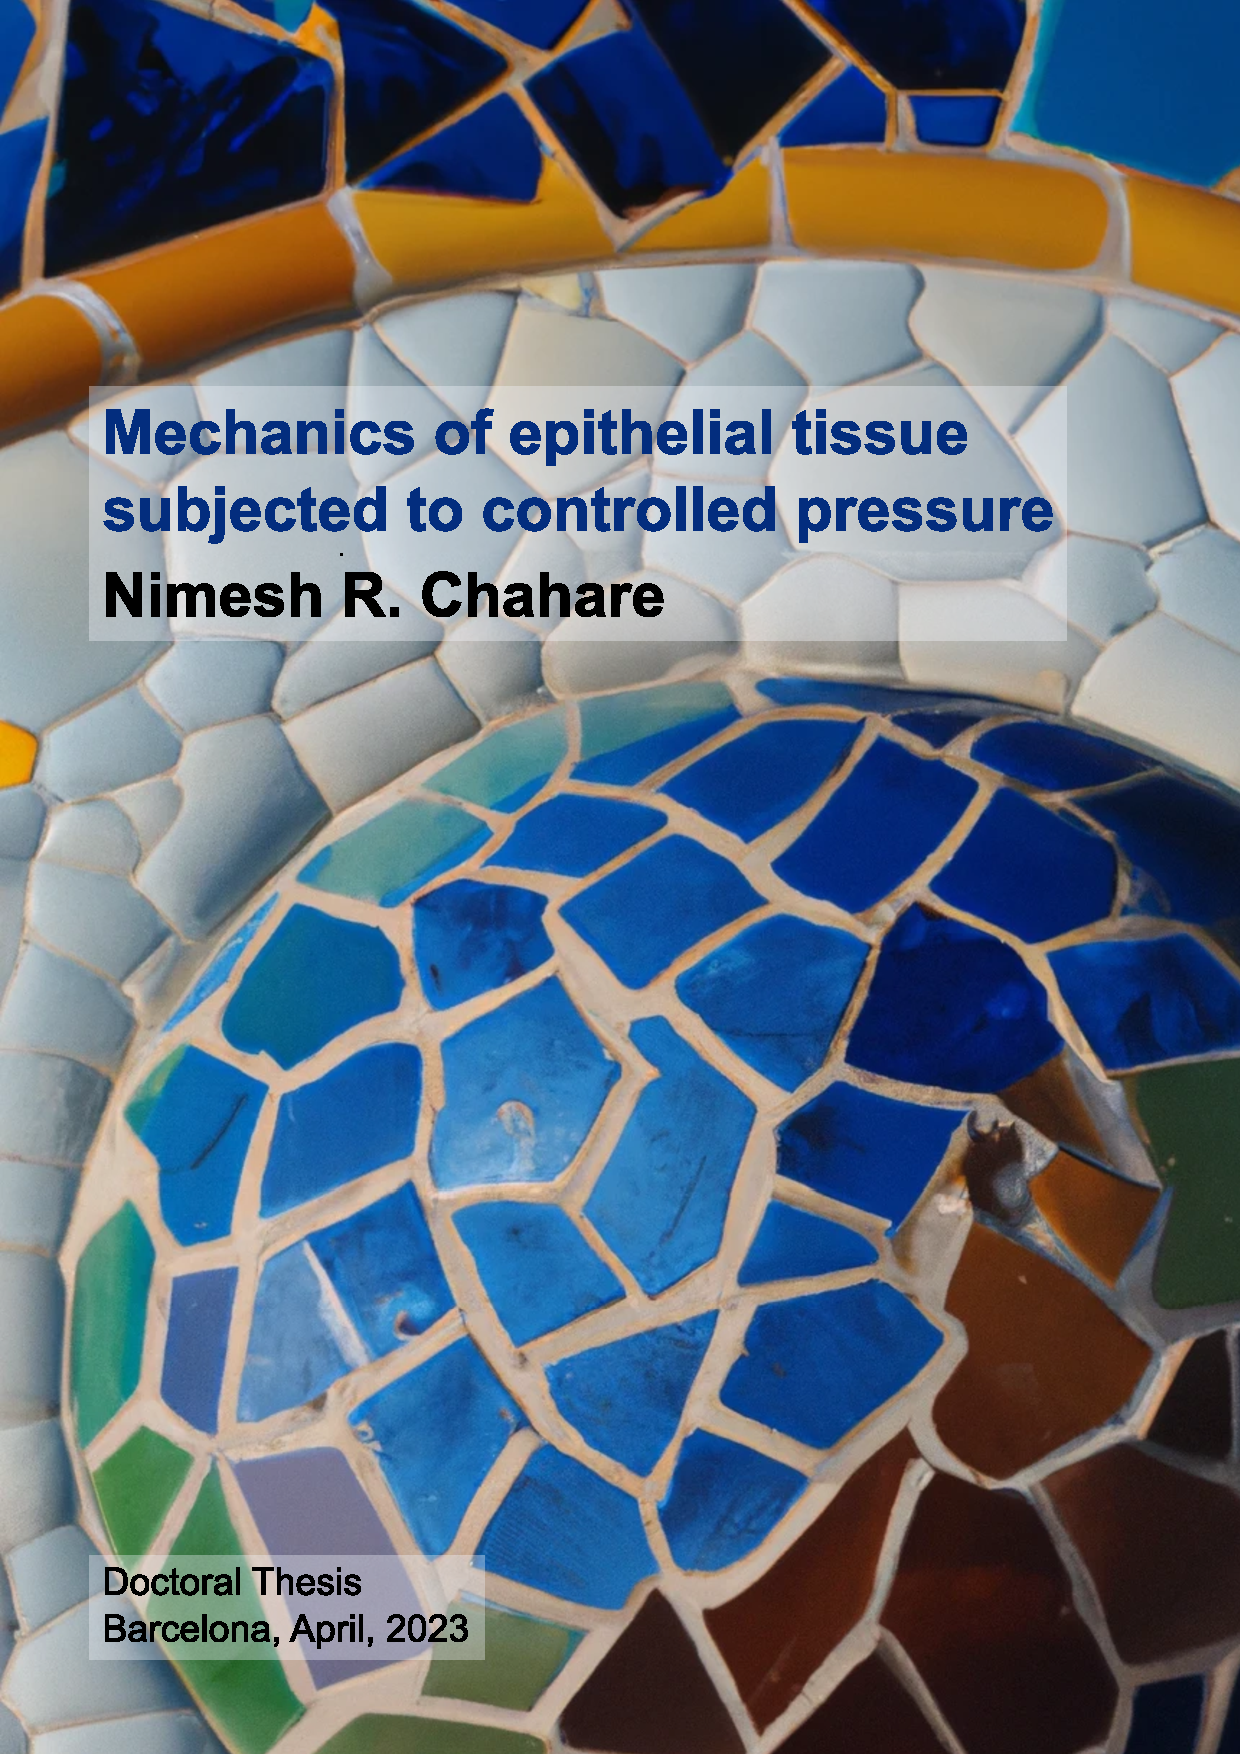
\includepdf[scale=1.01]{cover.pdf}

% 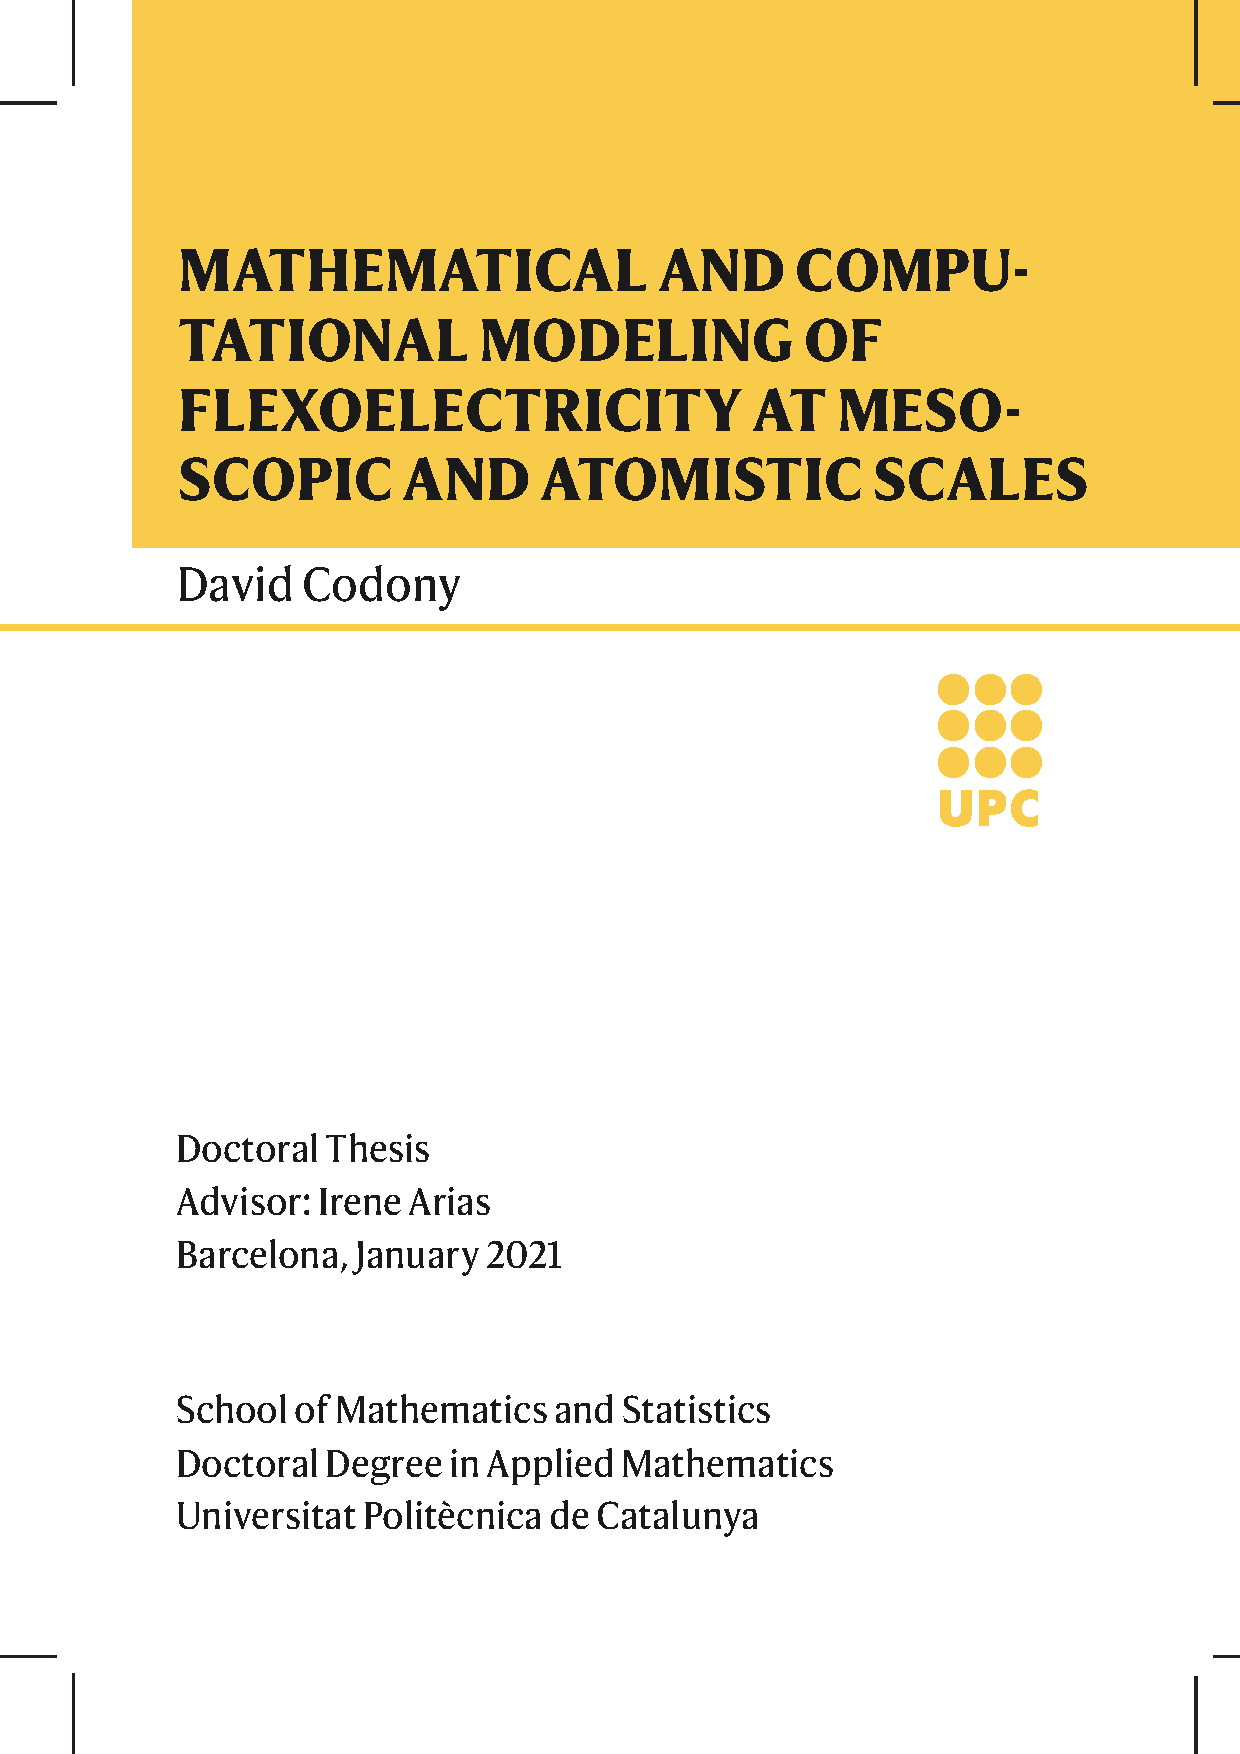
\includepdf[
%     %clip, trim={12.7mm 16.7mm 7.7mm 18.0mm},fitpaper
%     ,pages={1}
%     ,openright
%     ,noautoscale,scale=1
%     %,frame
%     ]{InnerCover.pdf}
\cleardoublepage 
	\setFiguresPath{LaCaN/0000-Preliminary/Logo}

\begin{center}

\includegraphics[height=45pt]{FME.png}
\hfill

\includegraphics[height=45pt]{FME_q.png}
\vspace{0.2cm} \hrule \vspace{0.3cm} 
\centerline{\Large\sc{\documenttype}}
\centerline{\large \sc{\universityschool}}
\centerline{\large \sc{\university}}

\vfill

{\sc\LARGE{\Title}\\}
\vspace{2.0em}
{\large {by}\\}
\vspace{1.0cm}
{\sc{\Large \Author}\\}

\vfill

\vspace{0.7cm}
\hrule \vspace{0.3cm}
\begin{minipage}{45pt}\flushright
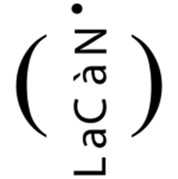
\includegraphics[height=45pt]{LaCaN.png}\end{minipage}~~
\begin{minipage}{0.45\textwidth}
{\large \sc{\universitydepartment}}
\end{minipage}

\vspace{1.0cm} 

\centerline{\large \textsc{\advisorname: \Advisor}}
\centerline{\large \textsc{\myCity, \mydate}}
\end{center}\cleardoublepage
	\strut 
\vfill
\begin{flushright}
\begin{minipage}[t]{.5\textwidth}\begin{flushright}
	\quote{``... If you want knowledge, you must take part in the practice of changing reality. If you want to know the taste of a pear, you must change the pear by eating it yourself...''}

\begin{CJK*}{UTF8}{gbsn}
	
毛泽东
	
\end{CJK*}

\end{flushright}\end{minipage}
\end{flushright}
\vfill 
\strut
\cleardoublepage

	
	%%% Preliminary %%%
	\frontmatter
	

\begin{Abstract}
Epithelial sheets form specialized 3D structures suited to their physiological roles, such as branched alveoli in the lungs, tubes in the kidney, and villi in the intestine. To generate and maintain these structures, epithelia must undergo complex 3D deformations across length and time scales. How epithelial shape arises from active stresses, viscoelasticity, and luminal pressure remains poorly understood. To address this question, we developed a microfluidic chip and a computational framework to engineer 3D epithelial tissues with controlled shape and pressure. In the setup, an epithelial monolayer is grown on a porous surface with circular low adhesion zones. On applying hydrostatic pressure, the monolayer delaminates into a spherical cap from the circular zone. This simple shape allows us to calculate epithelial tension using Laplace’s law. Through this approach, we subject the monolayer to a range of lumen pressures at different rates and hence probe the relation between strain and tension in different regimes while computationally tracking actin dynamics and their mechanical effect at the tissue scale. Slow pressure changes relative to the actin dynamics allow the tissue to accommodate large strain variations. However, under sudden pressure reductions, the tissue develops buckling patterns and folds with different degrees of symmetry-breaking to store excess tissue area. These insights allow us to pattern epithelial folds through rationally directed buckling. Our study establishes a new approach for engineering epithelial morphogenetic events.
\end{Abstract}

{\footnotesize
	\emph{Keywords}: epithelial monolayers, actomyosin cytoskeleton, morphogenesis, mechanobiology, microfluidics
}
\vfill 
\cleardoublepage

	%\phantomsection
\begin{Acknowledgements}
	To the working people of the world.
	
	
\end{Acknowledgements}
\cleardoublepage
	{ \hypersetup{linkcolor={black}}

\begin{singlespace}

\phantomsection\bgroup\hypersetup{hidelinks}
\addcontentsline{toc}{chapter}{\contentsname}
\tableofcontents
\egroup\cleardoublepage

%\phantomsection\bgroup\hypersetup{hidelinks}
%\addcontentsline{toc}{chapter}{\listfigurename}
%\listoffigures
%\egroup\cleardoublepage

%\phantomsection\bgroup\hypersetup{hidelinks}
%\addcontentsline{toc}{chapter}{\listtablename}
%\listoftables
%\egroup\cleardoublepage

%\clearpage
%\addcontentsline{toc}{chapter}{\boxesname}
%\listof{Box}{\boxesname}
%\cleardoublepage

%\phantomsection
%\addcontentsline{toc}{chapter}{\listalgorithmname}
%\listofalgorithms
%\cleardoublepage

\end{singlespace}
}
	
	
	%%% Body %%%
	\mainmatter
	\part{Introduction and motivation}\label{part_1}
	
	The central focus of this thesis is the epithelial tissue monolayer. From the perspective of a mechanical engineer, these monolayers are endlessly fascinating. These monolayers are remarkable in their ability to change shape, self-heal, and continuously deform or jam as needed \cite{xi2018}. They represent the simplest system for gaining a physical understanding of biological morphogenesis, as epithelia can be found everywhere in the body, covering the skin and lining various cavities and organs. The shapes of epithelial monolayers can range from simple spherical blastocysts to highly branched and folded lungs, and they are formed and maintained through constant adaptation and renewal. This thesis aims to explore the physical principles behind epithelial shape by combining theoretical and experimental approaches in the study of simple epithelial monolayers.
	
	The chapters in this part serve as a comprehensive overview of all the key topics related to my PhD research. They begin with a brief introduction to epithelial tissue and its constituent parts, followed by a discussion on the role of mechanics in morphogenesis and various modeling approaches. This part concludes with a review of the growing field of "bottom-up" morphogenesis, where researchers are building biological systems from scratch.

	\setFiguresPath{LaCaN/figure}

	\renewcommand{\thesection}{1.\arabic{section}}
	\hypertarget{epithelial-layers}{%
	\chapter{Epithelial Layers}\label{epithelial-layers}}
	

\hypertarget{introduction}{%
	\section{Introduction}\label{introduction}}

\begin{figure}[h!]
	\centering
	\includegraphics[width=0.7\textwidth]{chap1ruysch.png}
	\caption{\label{fig_1_1} \textbf{The Anatomy Lesson of Dr.~Frederik Ruysch}, 1670 by
		Adriaen Backer. \cite{ruyshc}}
\end{figure}

The term ``epithelia'' was first introduced by Dutch botanist Frederick Ruysch in the early 18th century (see fig \ref{fig_1_1}). He used it to describe the tissue he observed while dissecting the lips of a cadaver, and the word is derived from Greek roots ``epi,'' meaning top, and ``thele,'' meaning nipple.
\footnote{Ruysch is referred to as a ``Artist of death'' because of his famous anatomical collection. He was the first to use arterial embalming, which allowed for visualizing and dissecting smallest
	arteries. He also was part of the macabre practice of public dissections \cite{halley2019}.}
A few decades later, Swiss scientist Albrecht von Haller began using the term ``epithelium/epithelia'' to describe the fibers of the body, following the old Renaissance theory that the body was made of fibers, which were believed to be a fundamental building block of living things.
\footnote{Finding a fundamental unit of living entities comes from the philosophy of Gottfried W. Leibniz. It was based on the idea of ``monad''. Thanks to progress in microscopy and philosophy, naturalists were able to put together ideas for cells, fibers, and even cytoskeleton!\cite{zampieri2014}}
It was thought that these fibers and tissues arranged in different arrays gave rise to biological structures \cite{maccord2012, zampieri2014}. This theory was not far off, as epithelial tissues make up more than 60\% of the cells in a vertebrate's body and are found ubiquitously, covering the organs both inside and out \cite{alberts2015}.

\begin{wrapfigure}{r}{5cm}
	\caption{\textbf{Polarity of epithelia} Actin and myosin is distributed heterogenously in epithelial monolayers \cite{chen2018}.}\label{fig_1_2}
	\centering
	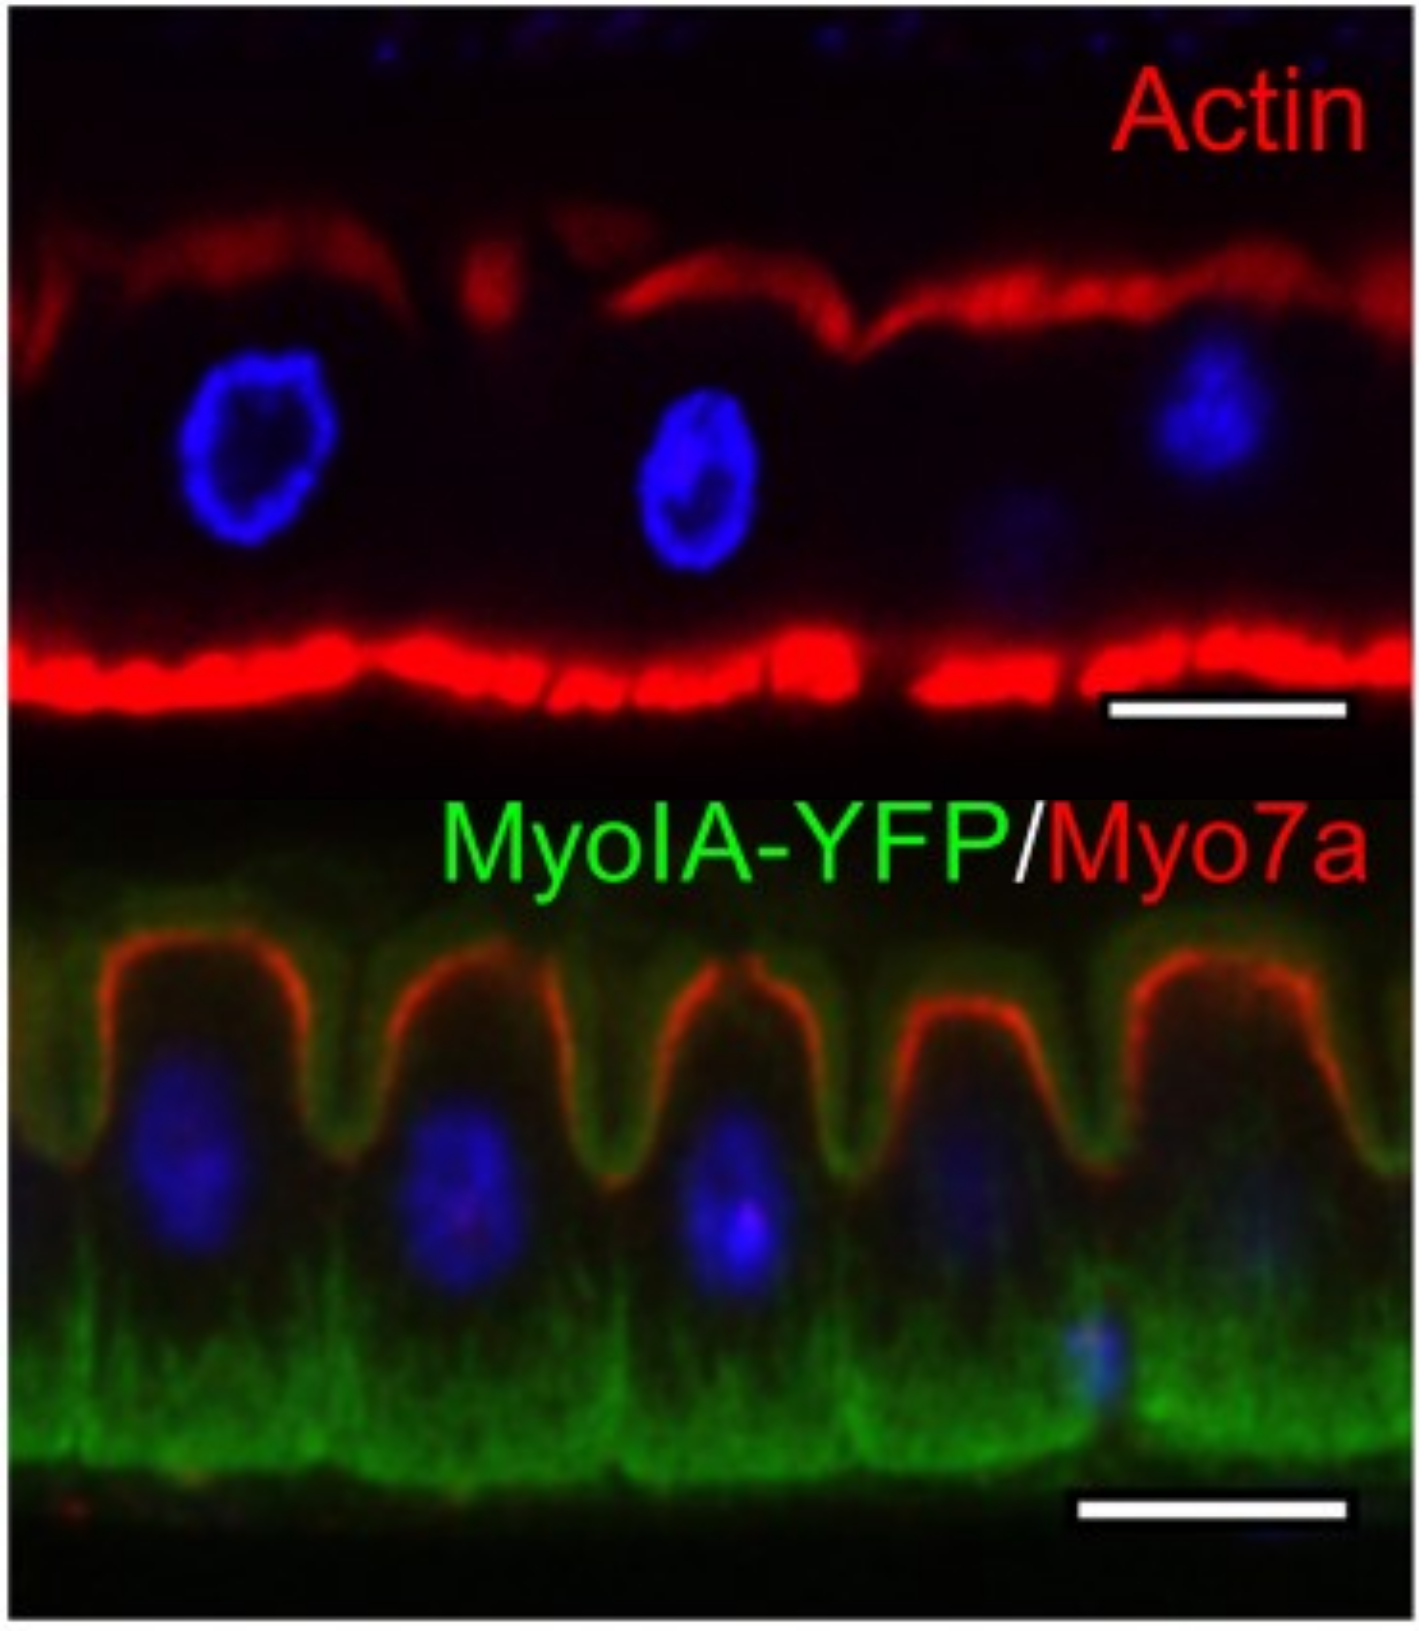
\includegraphics[width = 4cm]{chap1polarity.png}
\end{wrapfigure}

Epithelial cells are polarized, i.e., their apical side (typically facing the lumen of the organ), which differs in shape and composition from the basolateral side (see fig \ref{fig_1_2}). Its polar organization is reflected in the vectorial functions like creating and maintaining concentration gradients between separated compartments \cite{marchiando2010}. Typical examples of these are transporting epithelia such as those of the renal tubule, absorptive epithelia of the intestine, and secretory epithelial cells like hepatocytes \cite{alberts2015}. In addition, polarized epithelia guide the developmental process by determining the fate of cells leading to symmetry-breaking events in the embryo \cite{kim2018}.

\hypertarget{key-components}{%
	\section{Key components}\label{key-components}}

The function of epithelia primarily depends on the tissue's structure and the surrounding microenvironment. It can be divided into three aspects: cell structure, microenvironment, and cell-matrix interactions.

\hypertarget{cell-structure}{%
	\subsection{Cell structure}\label{cell-structure}}

The cell cytoskeleton plays a crucial role in maintaining cell shape and supporting vital functions such as cell division and migration \cite{alberts2015}. The Eukaryotic cell cytoskeleton is composed primarily of filamentous proteins, including three main types of filaments that differ in size and protein composition: microtubules, actin filaments, and intermediate filaments (see fig \ref{fig_1_3b}). Microtubules, with a diameter of approximately 25 nm, are the largest and made of the protein tubulin. Actin filaments, with a diameter of only 6 nm, are the smallest. Intermediate filaments, with a diameter of around 10 nm, are composed of several different subunit proteins and have a diameter intermediate between the other two types \cite{mofrad2009}. All three filament types dynamically respond to signals from the microenvironment and cell networks.

Mechanically, actin filaments have higher extensional stiffness than microtubules but break at lower extensions. Intermediate filaments have intermediate extensional stiffness and can sustain larger extensions while showing a nonlinear stiffening response \cite{wen2011}. Differences in strength and stability arise from the properties of individual subunits. The persistence length can range from 1\unit{\um} for intermediate filaments to 1\unit{\mm} for microtubules \cite{fletcher2010}. Actin filaments, most relevant to this thesis, have a persistence length of a few microns.

The assembly and disassembly of these filaments are dictated by the dynamics of their macromolecular components and accompanying proteins. The combination of actin filaments and myosin motors forms the actomyosin cortex, which is essential in producing intra- and intercellular forces. In an epithelial tissue, the actomyosin cortex and intercellular junctions make cell-to-cell contacts stronger and provide tissue integrity \cite{braga2016} (see fig \ref{fig_1_3}). A good example of these tissue-level structures can be observed in wound healing assays, where cells surrounding the wound create a ring of actin to close it \cite{brugues2014}. In Chapter 3, we will delve into the actomyosin network in more detail.

\begin{figure}[h!]
	\centering
	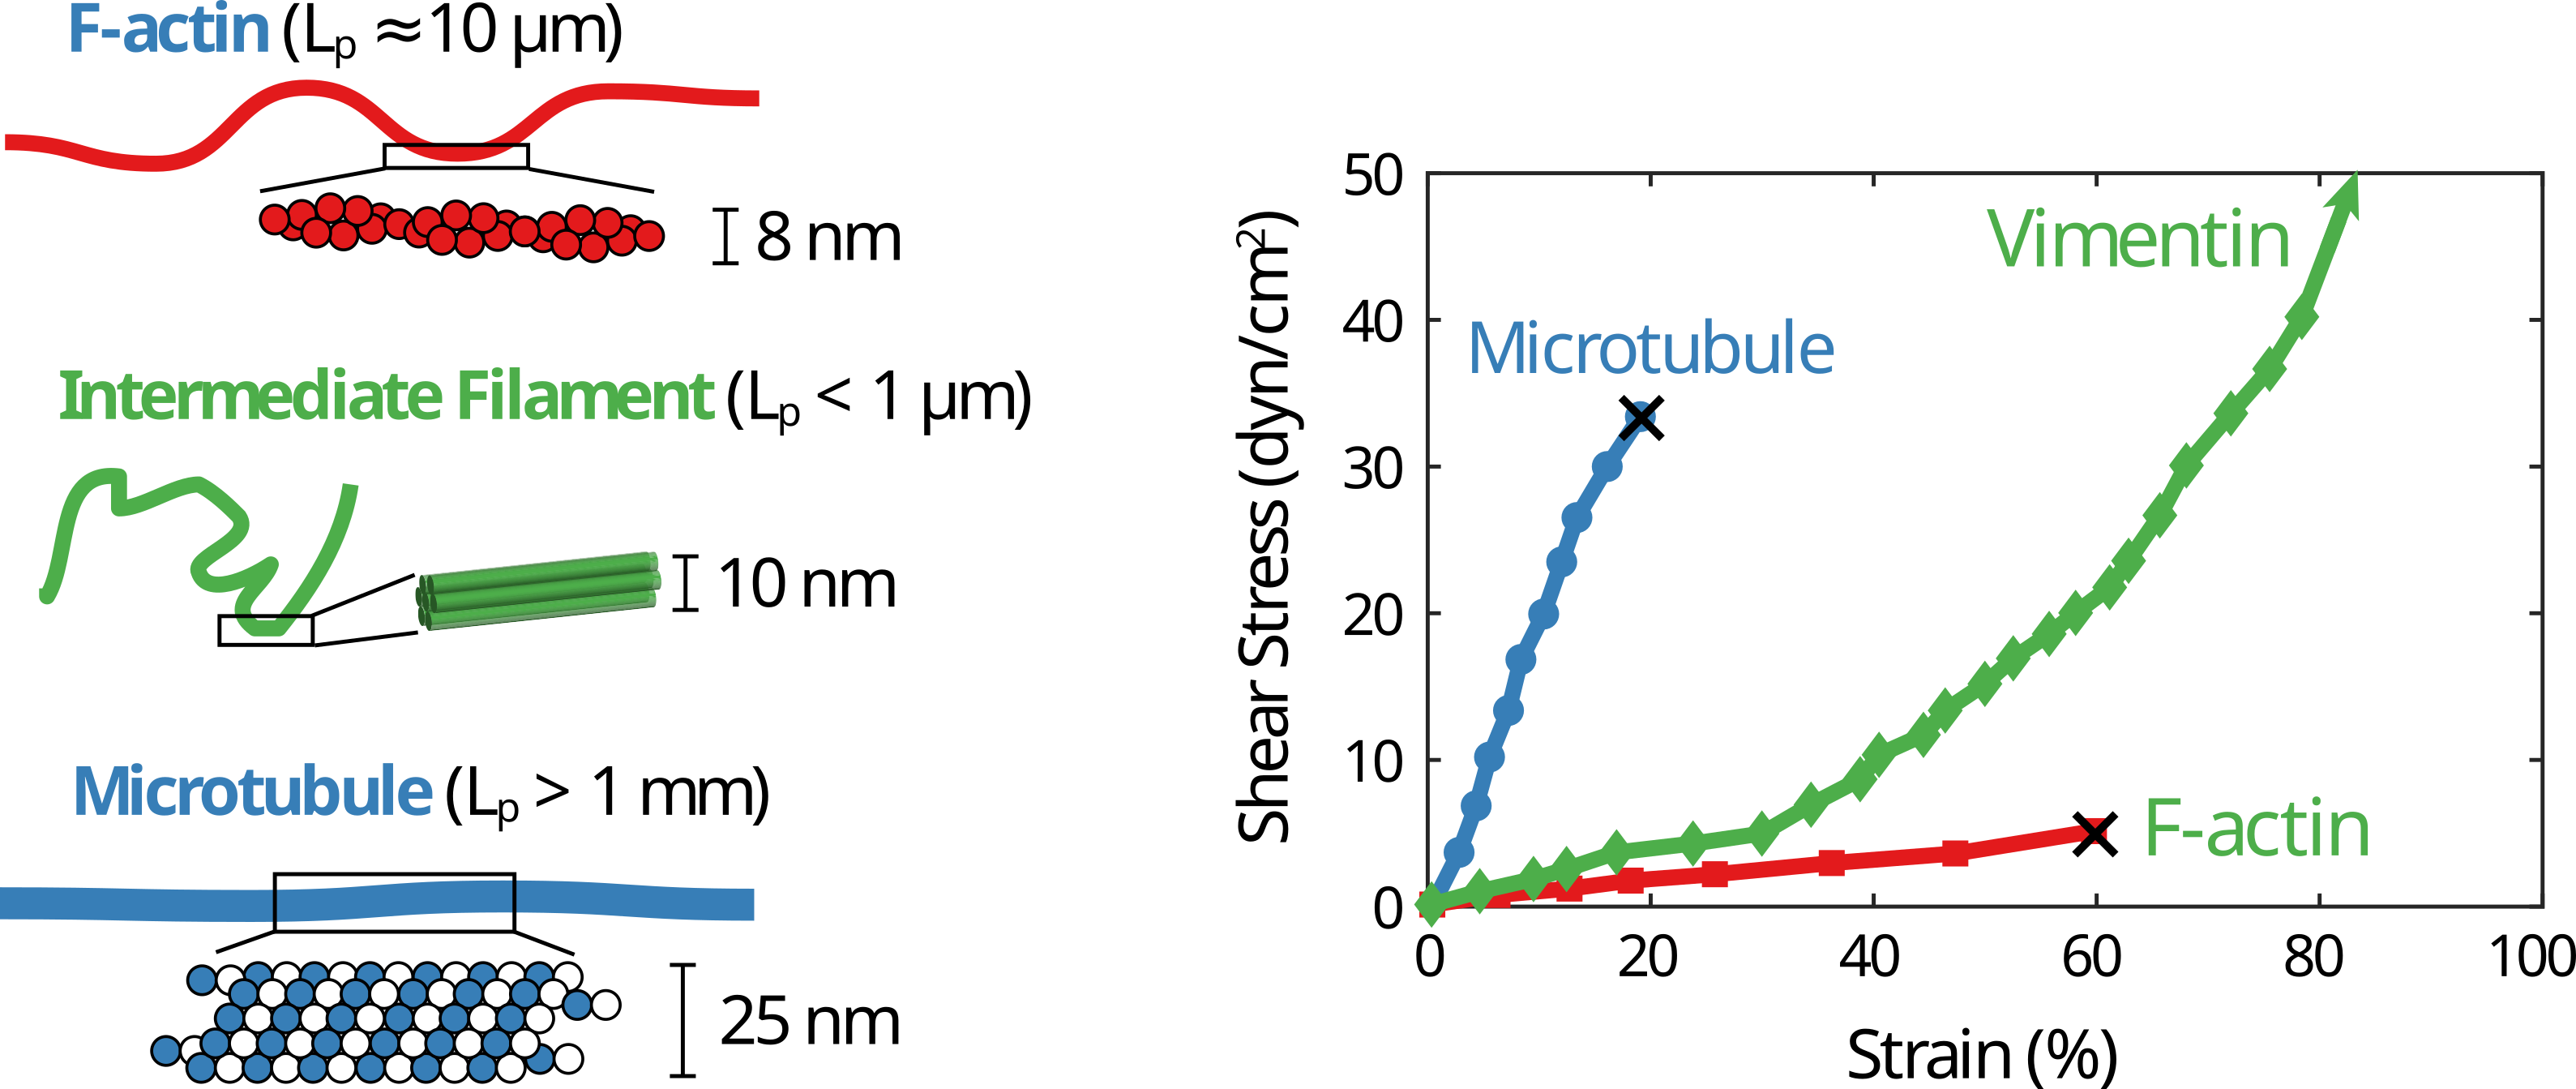
\includegraphics[width=0.8\textwidth]{chap1_filaments.png}
	\caption{\label{fig_1_3b} \textbf{Mechanics of cytoskeletal filaments}: Schematic and sizes of actin filaments, intermediate filaments and microtubules; along with the strain response to shear stress. \textit{Adapted from \cite{leggett2021}}}
\end{figure}

Multiple membrane molecules can facilitate cell adhesion, including cadherins. Cadherins are a crucial component for epithelial cell cohesion and the formation of adherens junctions, which transmit forces between cells. This key factor is involved in the mechanical regulation of cell division and tissue rearrangement during development and homeostasis \cite{godard2019, mertz2013}. Desmosomes, another type of intercellular junction, are coupled with intermediate filaments and provide mechanical resilience to cell layers \cite{hatzfeld2017, latorre2018}. Tight junctions serve as a barrier and regulate the active transport of ions across epithelial layers, playing an important role in controlling fluid pressure in tissues \cite{marchiando2010, chan2020}.

\begin{figure}[H]
	\centering
	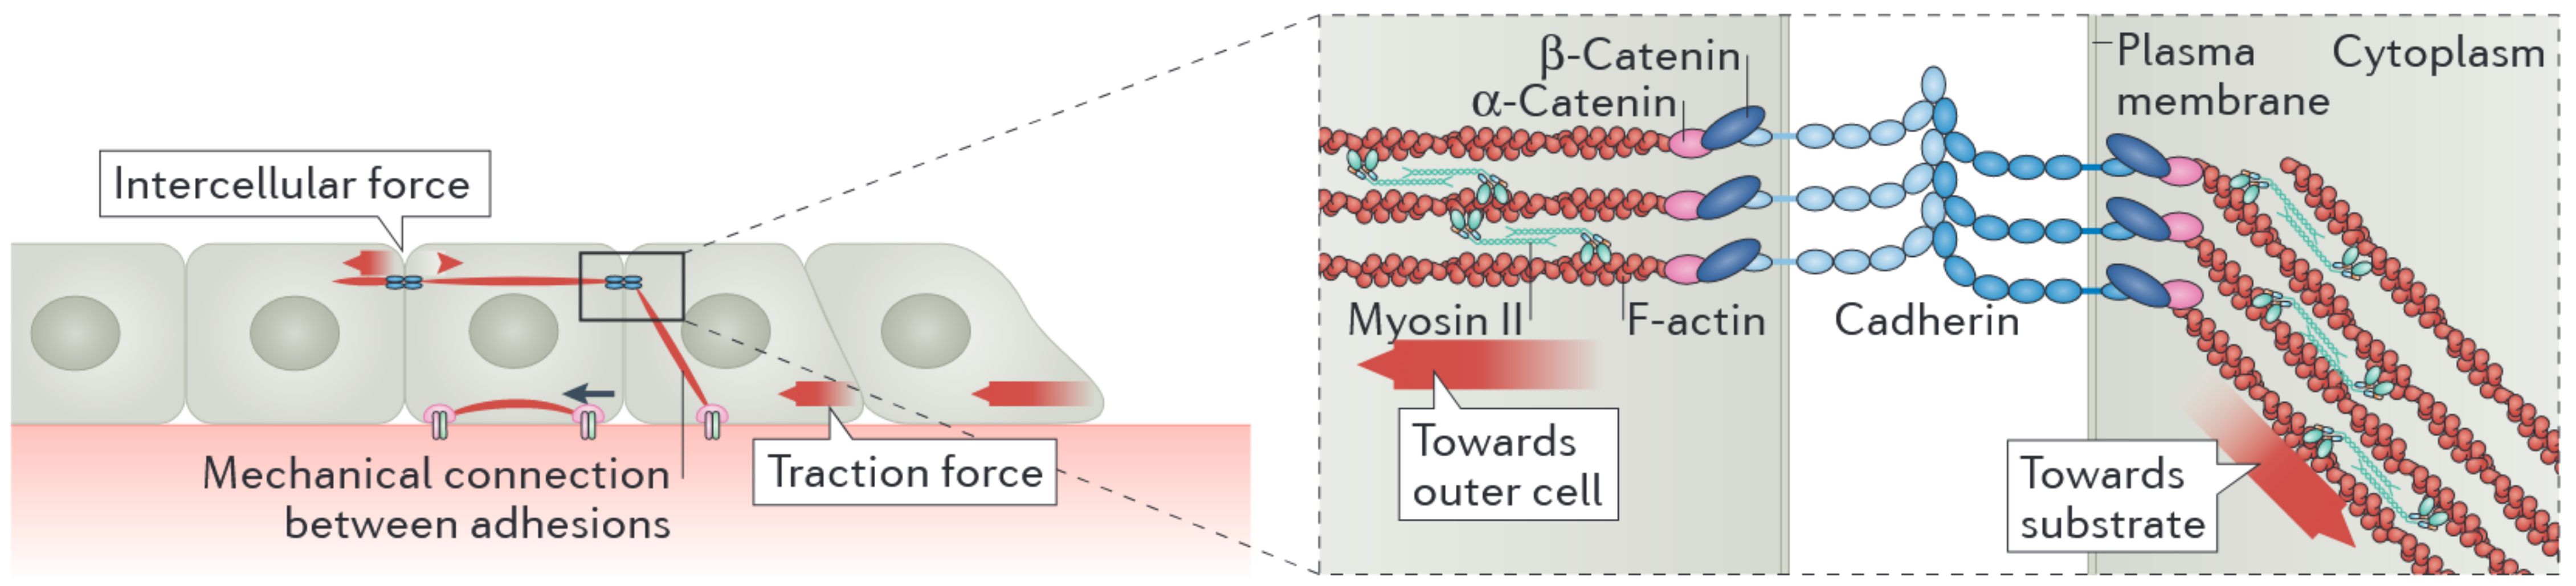
\includegraphics[width=\textwidth]{chap1_cellforces.png}
	\caption{\label{fig_1_3} \textbf{Intercellular forces through actomyosin cables and cadherins}: Schematic showing mechanical connections between adhesions and tissue force transmission with actomyosin cytoskeleton and adhesion proteins. \textit{Adapted from \cite{ladoux2017}}}
\end{figure}

\hypertarget{microenvironment}{%
	\subsection{Microenvironment}\label{microenvironment}}

The extracellular matrix (ECM) is the substrate or cell environment to which cells adhere. It is also referred to as the matrix, mesenchyme, or cellular microenvironment. The ECM serves many functions. It endows tissues with strength, thereby maintaining their shape. Additionally, it serves as a biologically active scaffolding that allows cells to migrate or adhere. The ECM also plays a role in regulating the phenotype of cells. It provides an aqueous environment that facilitates the diffusion of nutrients, ions, hormones, and metabolites between the cell and the capillary network \cite{alberts2015}.

Moreover, the ECM is subjected to mechanical forces such as blood flow in endothelia, air flow in respiratory epithelia, or hydrostatic pressure in the mammary gland and bladder \cite{waters2012, walma2020}. It has been shown that the ECM regulates cell shape, orientation, movement, and overall function in response to biophysical forces \cite{alberts2015}.

The ECM is a fibrous network of proteins, consisting of collagen, elastin, and proteoglycans as its primary structural components. Collagen is one of the most abundant proteins in the body, while elastin is the most elastic and chemically stable protein. Proteoglycans can sequester significant water as well as growth factors and proteases. The water content of the ECM allows it to deform as a poroelastic material, absorbing water upon stretching and releasing it under compression, causing a hydraulic fracture effect \cite{casares2015}. The collagen network can also remodel under the influence of cells and mechanical forces \cite{humphrey2014}.

Most ECM components undergo continuous turnover, some quickly and some slowly. For example, the half-life of collagen in the periodontal ligament is a few days, whereas that in the vasculature may be several months \cite{humphrey2014}. In response to altered physical stimuli, disease, or injury, the rates of collagen synthesis and degradation can increase many times, allowing for a rapid response.

\hypertarget{cell-matrix-interaction}{%
	\subsection{Cell-Matrix interaction}\label{cell-matrix-interaction}}

\begin{figure}
	\centering
	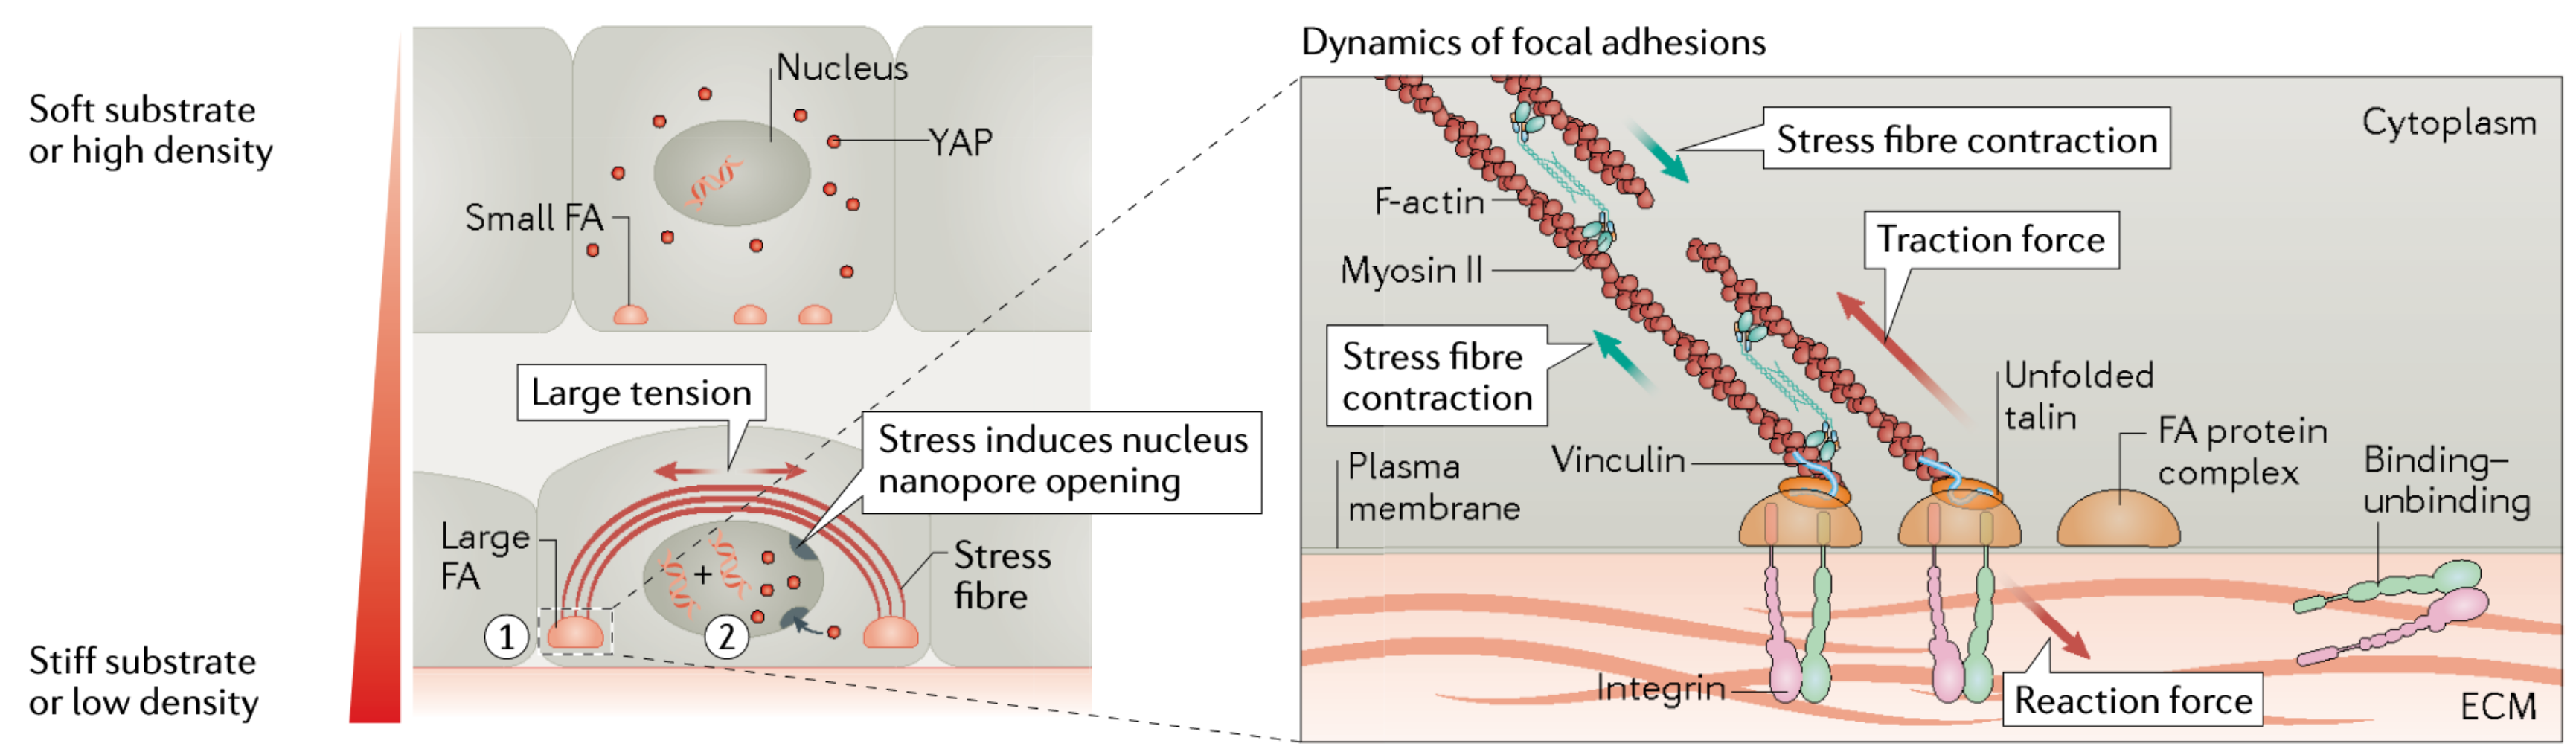
\includegraphics[width=\textwidth]{chap1_cell-matrix.png}
	\caption{\label{fig_1_4} \textbf{Cell-matrix interaction with respect to matrix stiffness and cell density}: In higher tension condition, the nucleus is deformed triggering mechanotransduction and causing alterations in cytoskeleton and tractions. \textit{Adapted from \cite{xi2018}}}
\end{figure}

The cells and the extracellular matrix (ECM) are in a dynamic relationship, constantly exchanging information and influencing each other. The cells sense the biophysical cues in the ECM through sensors such as integrins and focal adhesion complexes, which are responsible for cell-substrate adhesion \cite{kechagia2019} (see fig \ref{fig_1_4}). These adhesions allow cells to respond to various stimuli such as matrix stiffness, ligand density, and chemotactic gradients \cite{fortunato2022}. It has also been shown that cells can respond to the viscoelasticity of the matrix \cite{elosegui-artola2022}.

In addition to sensing the ECM, cells also contribute to its composition by secreting ECM components or remodeling the substrate \cite{malandrino2018}. This interplay between the cells and ECM can impact the tissue behavior fundamentally, as the connections between focal adhesions and the nucleus can affect the expression of transcriptional factors \cite{venturini2020, lomakin2020}. The precise control of cell-cell and cell-substrate interactions enables cells to transform into intricate shapes, such as curved forms in cell sheets \cite{schamberger2022}.

\hypertarget{role-in-disease-and-development}{%
	\section{Role in disease and
		development}\label{role-in-disease-and-development}}

Maintaining epithelial integrity and homeostasis is crucial for survival, and mechanisms have evolved to ensure these processes are sustained during growth and in response to damage. Epithelial cells have one of the fastest turnover rates in the body, with the entire gut cell lining turning over in 5--7 days \cite{barker2014}. This constant cell division and death pose a risk for tumor formation; it is know that 90\% of cancers emerging in simple epithelia \cite{torras2018, eisenhoffer2013}. Additionally, the high rate of cell turnover can disrupt the barrier function, as gaps should not emerge around dividing or dying cells.

If the fluid compartmentalization goes awry, it can have profound implications for epithelial and stromal homeostasis, fluid and electrolyte balance, and the development of inflammatory states. Several bacterial toxins are known to target junctions, causing changes in the tight junction protein ZO1, which compromises the barrier function and leads to pathologies such as diarrhea and colitis \cite{fasano1991}. In cancer, the compromised ZO1 barrier is essential to allow metastatic cells to break into and out of blood vessels. The leaky barrier also enables a growing epithelial tumor to access luminal fluids as an additional source of nutrients \cite{mullin2005}.

Furthermore, epithelia participate in physiological events such as epithelial--mesenchymal transition (EMT), which is a developmental process where epithelial cells gradually transform into mesenchymal-like cells by losing their epithelial functionality. EMT plays a vital role in normal biological functions such as repair and differentiation, as well as abnormal pathological activity such as organ fibrosis and promoting carcinoma progression \cite{alberts2015}. EMT endows cells with stem cell properties, enabling cell migration to distant organs and subsequent differentiation into multiple cell types during development and the initiation of metastasis \cite{thiery2009}. 

Epithelia undergo drastic shape changes with deformation and reorganization from the embryonic to the adult stage. It's not surprising that any malfunction in this process can lead to damage and disorder, resulting in congenital malformations, which are a major cause of infant mortality worldwide \cite{clarke2021}. Additionally, epithelial dysfunction is a precursor to diseases such as chronic obstructive pulmonary disease, asthma, cystic fibrosis, and pulmonary fibrosis \cite{carlier2021}.

\hypertarget{forms-of-epithelia}{%
	\section{Forms of epithelia}\label{forms-of-epithelia}}

The structure and arrangement of epithelial cells are crucial for maintaining the integrity and homeostasis of tissues and organs (see fig \ref{fig_1_5}). Simple epithelia are single-cell layers where all cells are in contact with the underlying basal lamina and have a free surface on the apical side. The shape of the cells can vary, ranging from flat to cuboidal to columnar. Stratified epithelia, on the other hand, have two or more layers of cells. Additionally, there are pseudostratified epithelia, which appear to be stratified, but are monolayers where the cell nuclei are positioned in a manner that gives the appearance of a stratified epithelium.

The classification of epithelia was first established in the XIXth century based on their structure and physiological characteristics. Germ layer theory, developed by embryologists, further expanded the epithelial nomenclature \cite{maccord2012}. During early embryogenesis, three layers emerge: endoderm, mesoderm, and ectoderm. The ectoderm forms the epithelia lining the skin, mouth, and nervous system, while the endoderm gives rise to the digestive tract, respiratory system, and liver. The mesoderm, in turn, develops the endothelia covering much of the circulatory and lymphatic systems.

It is important to note that not all tissues classified as epithelia, mentioned in this thesis, are purely composed of epithelial cells. They may be a mixture of different cell types that have epithelial-like characteristics. The focus of this thesis is on packed cell monolayers, which can form and self-organize into various 3D shapes, ranging from simple spheres to complex branched tubules. The thesis will explore the role of mechanics in epithelial morphogenesis.

\begin{figure}[H]
	\centering
	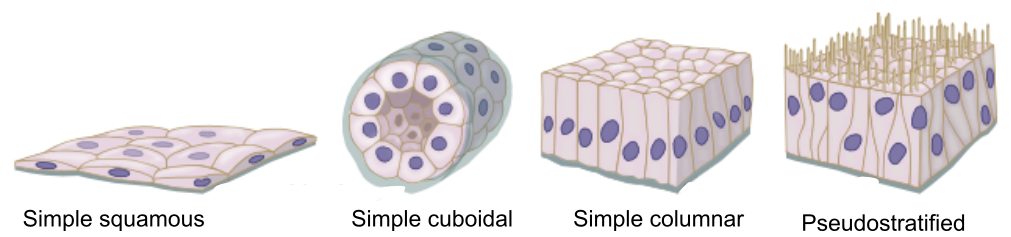
\includegraphics[width=0.75\textwidth]{chap1_forms.png}
	\caption{\label{fig_1_5} \textbf{Forms of epithelial tissues}: Simple squamous, cuboidal, columnar epithelia and pseudostratified epithelia. \textit{Adapted from \cite{zotero-9680}}}
\end{figure}

	\renewcommand{\thesection}{2.\arabic{section}}
	\hypertarget{the-mechanical-basis-of-morphogenesis}{%
	\chapter{The mechanical basis of
	Morphogenesis}\label{the-mechanical-basis-of-morphogenesis}}
	

\hypertarget{the-complexity-of-the-morphogenesis}{%
\section{The complexity of the
morphogenesis}\label{the-complexity-of-the-morphogenesis}}

Epithelial cells play a crucial role in the formation of transient structures during embryonic development, such as the neural tube, somites, and precardiac epithelium, which serve as the precursor for the development of complex organs. During this process, different types of epithelia acquire distinct morphological forms and perform specific functions, including branched lungs, looped gut, kidney tubules, thyroid follicles, and sinusoids in the liver. The regulation of epithelial morphogenesis is a complex and hierarchical process that involves coordinated events at multiple spatial and temporal scales \cite{trepat2018}.

Some processes appear to be happening fast at the local level, such as cell shape changes through apical constrictions, which lead to global changes, such as the formation of a ventral furrow in a Drosophila embryo \cite{martin2009}. At the same time, chemical signaling events that activate these processes are slow and occur at a global level. The same complexity can be seen in\textit{ in vitro} systems, where a cluster of dissociated stem cells can assemble into an organoid or gastruloid and undergo global folds in response to appropriate culture conditions \cite{collinet2021}.

The underlying mechanisms of epithelial morphogenesis are intricate and involve multiple factors, including genes responding to morphogen gradients, molecular machinery involved in apical constriction, and mechanical stresses that cause tissue-scale deformations. To fully understand the phenomenon of epithelial morphogenesis, it is essential to study these processes in detail, at multiple levels of complexity \cite{schock2002, lecuit2011}.

Rudolf Virchow's third tenet of the cell theory states that ``omnis cellula e cellula,'' meaning ``all cells come from cells'' \cite{virchow1860}.
\footnote{The famous epigram was coined by François-Vincent Raspail. Virchow is regarded as influential biomedical scientist of 19th century, but more interesting part is as a radical who took part in the March revolution of 1848. He was one of the first to advocate for the social origins of illness \cite{wright2012, brown2006}.}
Although all tissues originate from cells that contain essentially the same genetic information, each tissue has a distinct architecture and function. This raises several questions, such as: what makes cells different from each other? Are differences due to genes, environmental factors, or both? What drives shape changes in tissue morphogenesis? Over the last two centuries, the field of developmental biology has addressed many of these questions, but it has also raised new issues and left others unanswered.

Until last decade, the focus of the field had been on tracking and mapping patterns of cell movements to patterns of gene or protein expression \cite{gorfinkiel2021}. While these studies are influential and important for understanding morphogenetic patterns, they fall short in explaining how cells and tissues are physically shaped \cite{veenvliet2021, odell1981}. This is because the physical understanding of tissues has been limited to kinematic descriptions, which only describe tissue deformation or cell motion. However, we know that cells and tissues actively drive shape changes and movements through the generation of mechanical forces \cite{lecuit2011}. Thus, to have an integrated understanding of morphogenesis, we must consider the role of forces and mechanics.

\hypertarget{on-growth-and-form}{%
\section{On growth and form}\label{on-growth-and-form}}

Throughout history, the form of both animate and inanimate objects has been closely linked to their intended function. In fact, the XXth century architecture principle ``Form Follows Function'' highlights the idea that the organization of a structure should be based on its intended purpose. Similarly, in developmental biology, self-assembling systems such as intestinal organoids, cancer spheroids, and gastruloids are perfect examples of this principle in action, as each structure emerges from a set of cells in a suitable environment, adapting to perform a specific biological function \cite{gjorevski2016, ishiguro2017, morizane2017, vianello2019}.

However, the opposite design principle appears to be at work in numerous \textit{in vitro} experiments that involve a controlled cellular environment. In such experiments, geometric constraints appear to drive biological function \cite{xi2018}. For instance, seeding stem cells in a bio-printed three-dimensional geometry of the gastrointestinal tract led to the production of functional tissues with physiological characteristics of
the intestine. The curvature of the structure can even control the formation of villus-like structures \cite{brassard2021}. 

\begin{figure}[h!]
	\centering
	\includegraphics[width=\textwidth]{chap2shah.png}
	\caption{\label{fig_2_1} \textbf{Multiscale imaging and tracking of embryo cell dynamics}: Top panels show in toto imaging of germlayer specification; red is mesendoderm, blue is epiblast, and yellow is endoderm. Bottom panel shows data analysis of long term pan embryo cell dynamics \cite{shah2019}}
\end{figure}

In a way, assembly of biological systems treads the line between self-organization and programmed material. Advanced microscopy techniques have allowed us to witness the intricacies of developmental processes with unprecedented clarity (see fig \ref{fig_2_1}). We can now observe cells and their motion throughout the morphogenetic process, from the formation of a spherical embryo to the creation of a complete organism \cite{shah2019}. Cells undergo shape changes and large-scale flows as they undergo morphogenesis, driven by mechanical forces in concert with biochemical processes \cite{labernadie2018, trepat2018, lecuit2011}. Thus, the dichotomy of form and function is incomplete without considering the physical laws of mechanics.


Over a century ago, D'Arcy Wentworth Thompson wrote the influential book ``On Growth and Form'' \cite{thompson1979}, in which he explored the relationship between geometry, physics, and biology in the context of morphogenesis. Thompson used examples to show how mathematical principles can explain biological phenomena, such as his theory of transformations, which demonstrates how related species can be represented geometrically (see fig \ref{fig_2_1b}). According to Thompson's daughter, he even used to draw pictures of dogs on rubber sheets and stretch them to show children how poodles could become dachshunds \cite{wolfram2022}. This distortion of shape represents significant alterations in various forces or rates of growth throughout the developmental processes of different organisms.

Thompson's approach was highly speculative, but his goal was to identify general principles behind the diverse forms and patterns found in biology. He compared growth curves of haddock, trees, and tadpoles, and found logarithmic spirals in shells, horns, and leaf arrangements.
\footnote{Funnily, He criticized the zoologists and morphologists of the time of assigning shapes to psychical instinct of the organism or some divine interference for creating the perfect shapes: “He finds a simple geometric construction, for instance in the honeycomb structure, he would fain refer it to psychical instinct or design rather than in the operation of physical forces. ... When he sees in snail, or nautilus, or tiny foraminiferal or radiolarian shell a close approach to sphere or spiral, he is prone of old habit to believe that after all it is something more than a spiral or a sphere, and that in this "something more" there lies what neither mathematics nor physics can explain}
Essentially, this book emphasized two points: first, all material forms of living things---cells, tissues, and organs---must obey the laws of physics, and second, quantitative measurements are necessary to unravel the physical principles of biology.

\begin{figure}[h!]
	\centering
	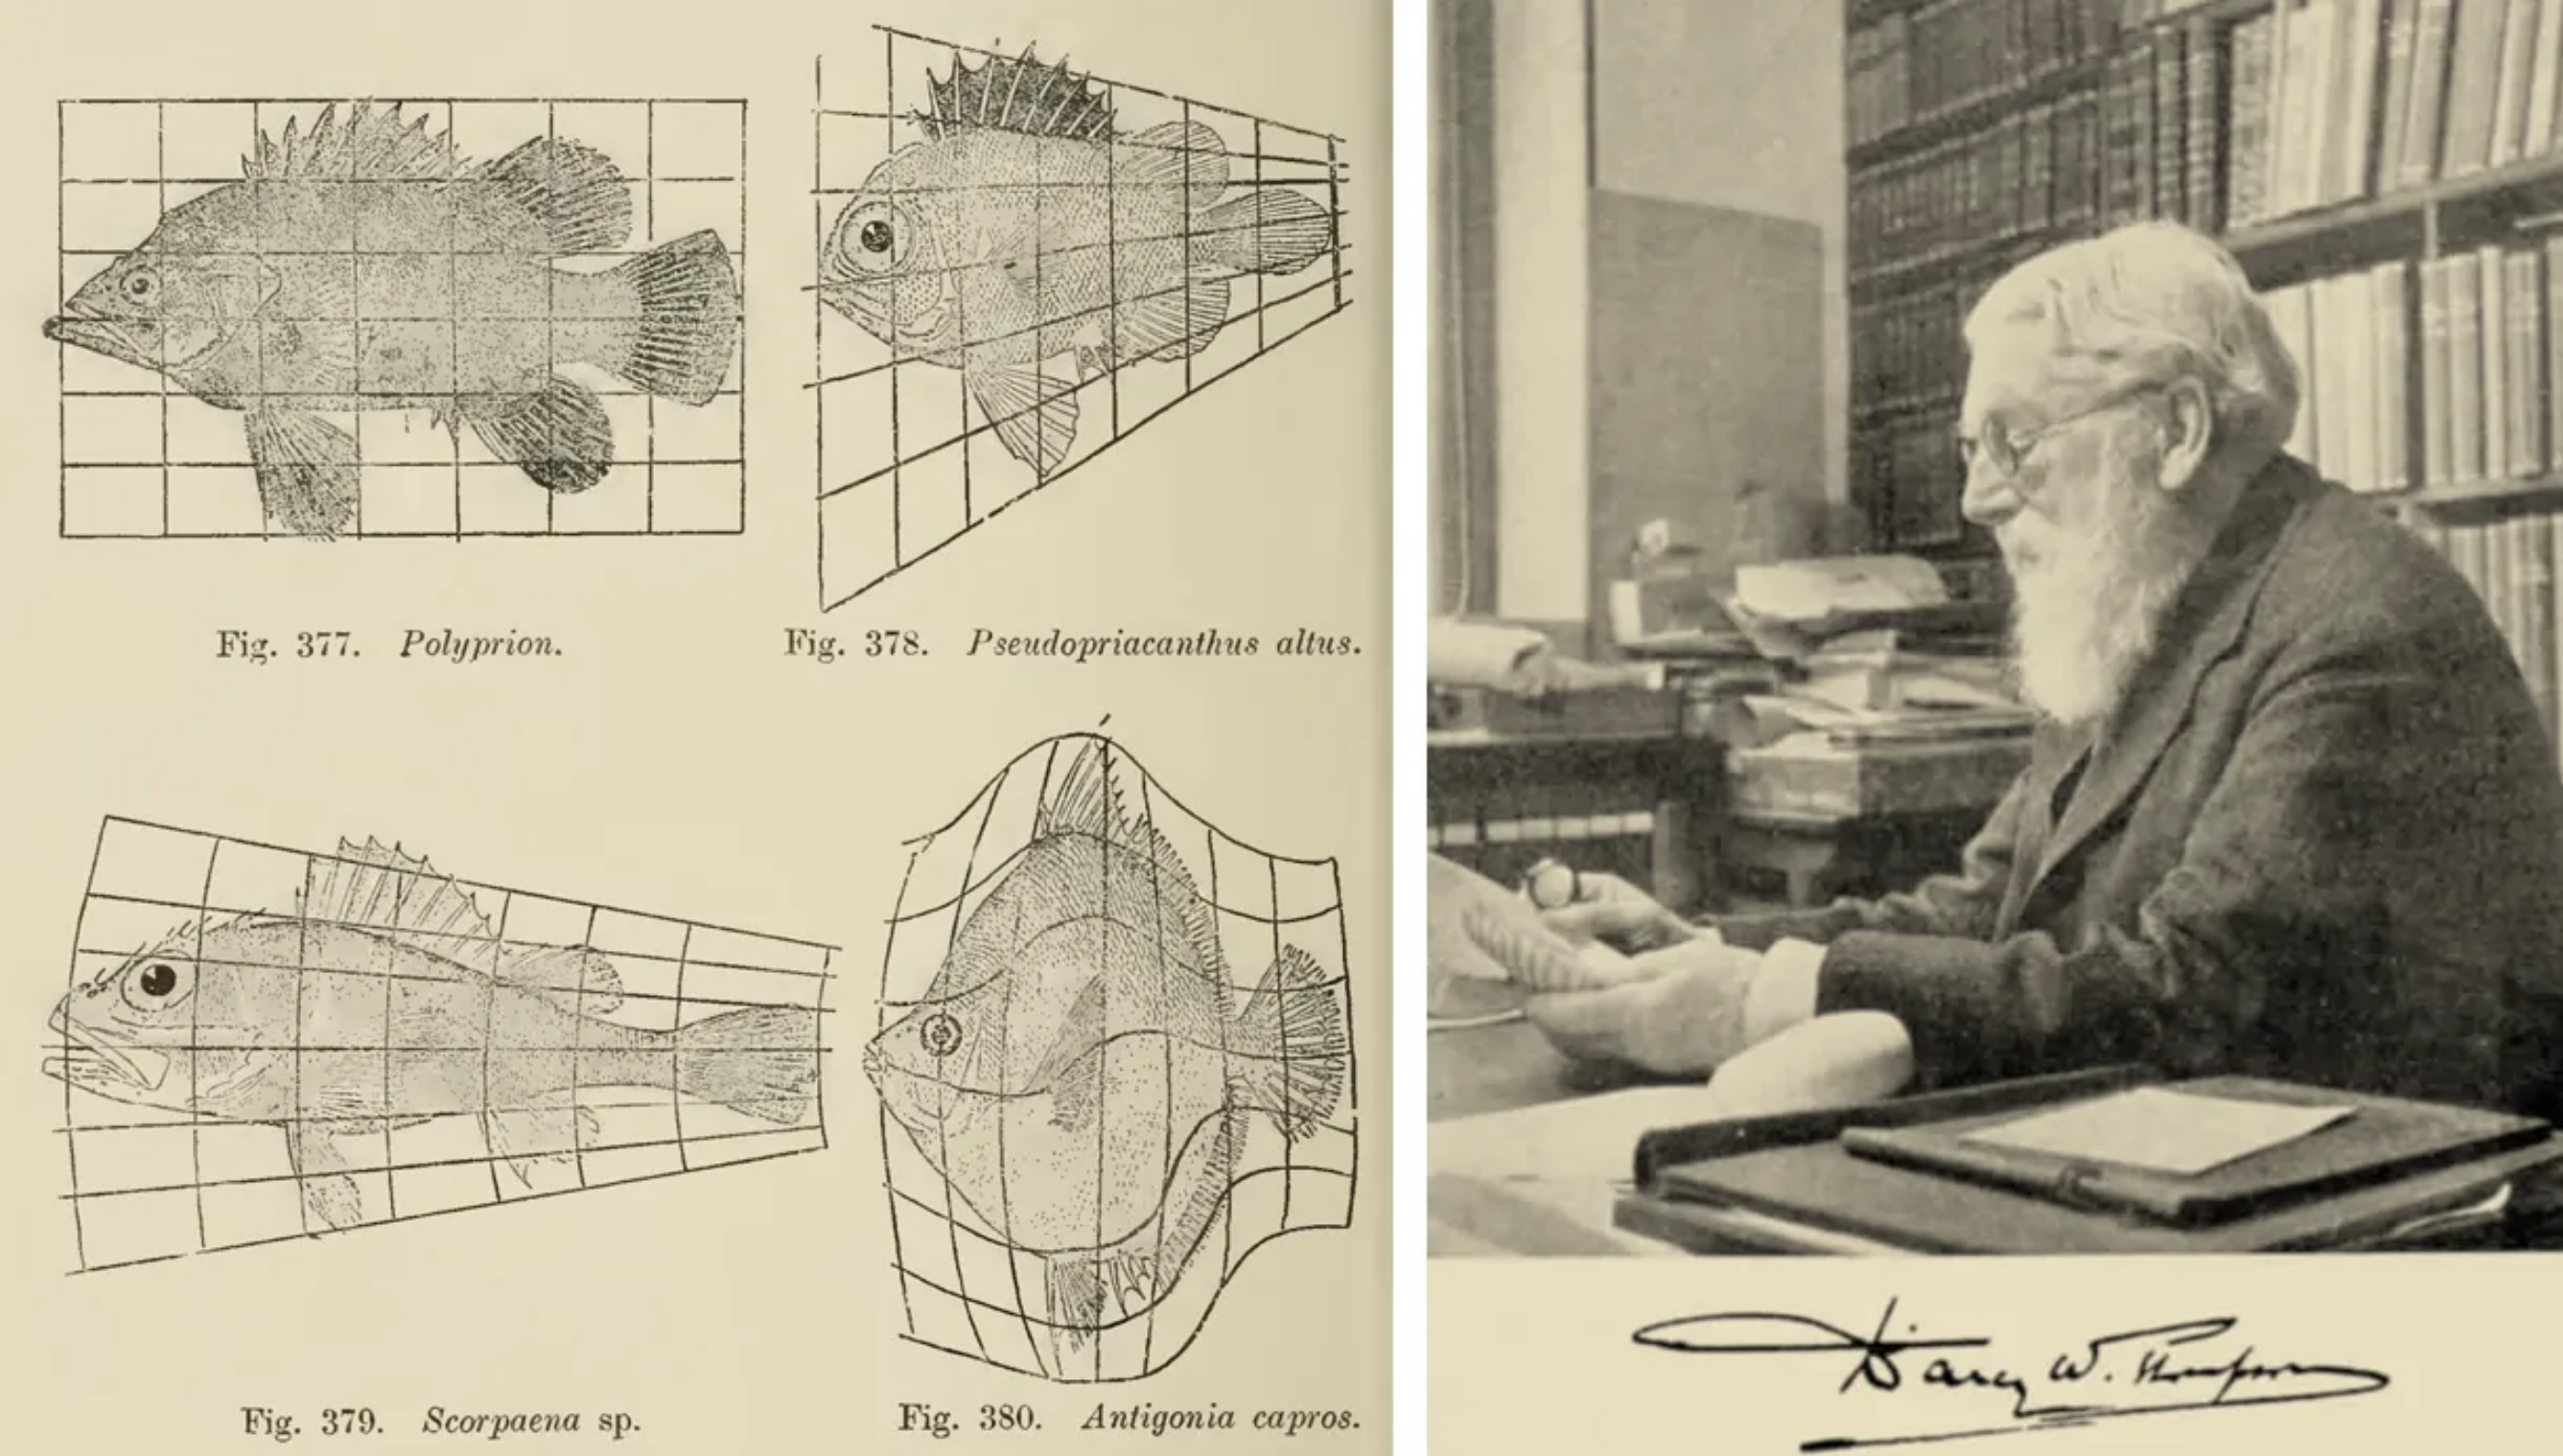
\includegraphics[width=0.75\textwidth]{chap2darcy.png}
	\caption{\label{fig_2_1b} \textbf{D'Arcy Thompson's fishes} and his theory of transformation. \cite{wolfram2017, thompson1979}}
\end{figure}

Thompson's work continues to inspire researchers even today. Right as I began my Ph.D., the centenary of the book's publication was being celebrated in the fields of developmental biology and biophysics \cite{heer2017, nat2017, natphys2017}. Even more so by the field of mechanobiology, an interdisciplinary field that studies the role of biophysical forces in cell and tissue functioning. 

\hypertarget{mechanobiology}{%
\section{Mechanobiology}\label{mechanobiology}}

The cells within epithelial tissue can be viewed as mathematical systems that integrate multiple input cues to result in an output behavior. These inputs can be mechanical or chemical, such as the stretching of lungs or the presence of morphogen gradients during embryonic development. The outputs can include cell deformation, migration, differentiation, or proliferation \cite{kumar2017}. Some outputs can even feedback into the system as an input, such as when cells remodel the matrix \cite{malandrino2018}. Mechanochemical switches at the membrane, cell-cell junctions, or cell-matrix adhesions mediate the sensing of the environment, triggering a biochemical cascade that leads to a cellular response \cite{roca-cusachs2017}. This interplay between biochemistry and mechanics is known as mechanotransduction.

During morphogenesis, mechanotransduction occurs at various scales, ranging from a single cell to complex multicellular tissue. To understand the role of different variables, experiments at different scales are necessary. It has been observed that individual cells can sense their environment and respond by altering their behavior through mechanical or biochemical processes. Whereas, multicellular systems can transmit forces and information at a longer length scale, allowing for emergent characteristics such as collective migrations, oscillations, rearrangements, and even turbulent flows \cite{heer2017, lecuit2011,trepat2018}.

An excellent demonstration of the interaction between tissues and their environment is provided by the phenomenon of durotaxis. Epithelial cells can detect changes in the stiffness of the extracellular matrix and migrate towards areas of higher rigidity. This migration towards stiffer regions has been observed both \textit{in vitro}, where cells in a monolayer collectively expand and relocate to stiffer areas, and \textit{in vivo}, such as during the migration of neural crest cells in \textit{Xenopus laevis} \cite{sunyer2016, shellard2021}. It is worth noting that the migration of neural crest cells themselves generates the durotactic gradient. In another example, during Drosophila oogenesis, the disorganized matrix is remodeled by cells to create a polarized matrix that aligns with the actin bundles in the follicular epithelium. This alignment is achieved through the coordinated rotation of cells and can guide the directed motion of cells along the polarized fibers \cite{haigo2011, cetera2014}.

The interplay between individual cells, their neighbors, and exogenous stimuli makes it difficult to decouple various biophysical aspects of the environment, such as forces, pressures, matrix stiffness, spatial confinement, porosity, or viscoelasticity. Direct force measurements in and out of tissues are also challenging. To address these challenges, researchers from various disciplines have attempted to recreate experimental systems with precise control over the biochemical and mechanical environments of cells \cite{xi2018}. This has been made possible through continuous technological advancements in fluorescent probes, imaging, microfabrication, and force measurements \cite{roca-cusachs2017}. In the following section, I will provide an overview of relevant techniques and experiments in the field of mechanobiology.

\hypertarget{synthetic-substrates}{%
\subsection{Synthetic substrates}\label{synthetic-substrates}}

The use of Polyacrylamide and soft PDMS gels has enabled researchers to investigate mechanical interactions at cell-substrate adhesion (see fig \ref{fig_2_2} A). Simply seeding cells on hydrogels of different stiffnesses reveals a significant impact on the actin cytoskeleton, cell shape, and lineage specification \cite{yeung2005,  engler2006}. These substrates, because of their known elastic response, are also utilized in techniques like traction force microscopy (TFM) to measure the forces exerted by cells and tissues on the substrate \cite{harris1980,  gomez-gonzalez2020} (see fig \ref{fig_2_2} D). TFM studies have shown that cells and tissues can exert greater forces on stiffer substrates as a result of the remodeling of the cytoskeleton \cite{elosegui-artola2016}. Higher matrix stiffness has also been found to induce the translocation of Yes-associated protein (YAP) from the cytoplasm to the nucleus, which is considered a sensor for mechanotransduction \cite{elosegui-artola2017}. However, increasing extracellular matrix (ECM) ligand density alone can induce YAP nuclear translocation without changing substrate stiffness \cite{stanton2019}.

\hypertarget{geometric-control}{%
\subsection{Geometric control}\label{geometric-control}}

The shape of cells or tissues on 2D substrates can be controlled using micropatterned adhesion proteins or microfabricated stencils. Protein patterning techniques are used to pattern adhesion promoting proteins and control cell attachment and spreading, while microfabricated stencils physically confine cells in a particular geometry (see fig \ref{fig_2_2} B C). When cells are confined, they respond by reorganizing their actin cytoskeleton and focal adhesion complexes to match the shape imposed on them \cite{vignaud2012}. Confined tissues undergo larger-scale rearrangements, leading to the formation of fascinating topological defects or oscillations \cite{tlili2018,  balasubramaniam2021,  guillamat2022}. Through these experiments, we can uncover the mechanisms of force transmission and regulation of collective cell migration and epithelial growth in two dimensions \cite{nelson2005,  vedula2012,  deforet2014}.

Embryonic stem cells subjected to 2D confinement have been shown to differentiate based on the shape and size of the confinement. For example, a circular monolayer of stem cells can reproduce the tissue patterning of a 3D gastruloid \cite{warmflash2014}, and confinement in a triangular shape can lead to high tension at the vertices and activate Wnt signaling, promoting differentiation to mesoderm \cite{muncie2020}. Moreover, advancements in photopatterning technologies allow for precise control of multiple proteins on the same substrate \cite{guyon2021, prahl2022}, enabling the establishment of complex co-culture systems that mimic \textit{in vivo} events.

Not just 2D shape, epithelial monolayers are also able to respond to curvature by regulating cell migration, orientation, cell/nucleus size, and shape \cite{marin-llaurado2022, schamberger2022} (see fig \ref{fig_2_2} C). For example, an epithelial monolayer on hemispheres of elastomers acts as a fluid with increasing curvature \cite{tang2022}. On a smaller scale, cells attached to corrugated hydrogels show variations in lamins, chromatin condensation, and cell proliferation rate in response to curvature \cite{luciano2021}. Bio-printing of three-dimensional tissue architectures can also create functional tissues \cite{brassard2021,  breau2022}.

\begin{figure}[h!]
	\centering
	\includegraphics[width=\textwidth]{chap2mechnobiology.png}
	\caption{\label{fig_2_2} \textbf{Mechanobiological strategies for studying morphogenesis} \textit{Adapted from \cite{vianello2019}}}
\end{figure}

\hypertarget{mechanical-control}{%
\subsection{Mechanical control}\label{mechanical-control}}

Living systems have mechanical control in addition to spatial control, as physical forces emerge from growth, deformation, and remodeling of the extracellular matrix (ECM) and fluid pressure in closed geometries. For example, the intestinal epithelia are stretched during peristaltic movements in the gut and lung alveoli deformations during breathing. Compression can also guide morphogenetic events that involve tissue bending and folding, such as the formation of the optic cup, gut villi, and cortical convolutions in the brain \cite{okuda2018, shyer2013, tallinen2016}.

To study tissue behavior under external perturbation, cells and tissues are probed at the molecular and subcellular scales using techniques such as atomic force microscopy, magnetic beads, optical tweezers, and micropipettes \cite{bao2003} (see fig \ref{fig_2_2} E). At a larger scale, various types of stretching devices, tissue rheometers, and force plates can be used \cite{xi2018}. These experiments reveal that cells exhibit complex viscoelastic behavior at different levels of deformation and different regions of the cytoskeleton \cite{mofrad2009}. The response of tissues to stretching can vary depending on the timescale of the stretch and the reorganization of
cells within the tissue \cite{guillot2013}. Rheological experiments also help to uncover the role of signaling pathways, such as YAP transcription factors, in mechanosensation \cite{wagh2021}.

The microfluidic system, also known as ``cells on a chip,'' has emerged as a valuable tool for investigating cell behavior under controlled biophysical conditions that mimic \textit{in vivo} conditions \cite{ingber2018}. This
system allows for the application of stretch or shear forces, as well as the creation of a controlled microenvironment that mimics the organ-level cues present in the body. For instance, the surface tension at the air-liquid interface in the lungs and the fluid flow through the vasculature, as well as the cyclic mechanical stretch of the tissue-tissue interface due to breathing, can be replicated using this approach \cite{huh2010}.

In the context of developmental biology, the use of microfluidic systems has allowed for the study of self-organization and embryo functions under controlled physical conditions. The co-culture of iPSC-derived motoneurons and brain microvascular endothelial cells in a microfluidic system has produced the \textit{in vivo}-like maturation of spinal cord neural tissue, representing a new avenue for exploring the complex interplay between physical and biological factors in development \cite{sances2018, samal2019}.

As mentioned earlier, the tissue-matrix interaction plays a critical role in sensing and rapidly transmitting forces \cite{tambe2011, sunyer2016, serra-picamal2012}. However, in early embryonic epithelia where little or no ECM is present, stresses generated by actomyosin contraction of the cells in one tissue are transmitted over long ranges via intercellular adhesions to other tissues. Thus, studying a simple free-standing epithelial monolayer is very appealing in terms of characterizing the mechanical response to stretch at different time scales.

Only two techniques are available for this: first, Harris and colleagues created a suspended monolayer by culturing a cell monolayer on a collagen matrix on two rods, and later removed the matrix using enzymatic digestion \cite{harris2012}. Second, epithelial domes, where MDCK cells pump ions to form fluid-filled blisters, have been used \cite{lever1979}. Recently, my colleagues, Ernest Latorre and Ariadna Marin-Llaurado, have enhanced control over the curvature, shape, and size of the domes \cite{latorre2018, marin-llaurado2022}, details on this system in the next chapter. These experiments showed that elasticity measurements of the monolayer were two orders of magnitude larger than those of individual cellular parts, and the monolayer could sustain more than 200\% strain before the rupture of cell-cell junctions. The cell cytoskeleton, particularly the actomyosin network and cadherin junctions, actively remodel during stretching, while the keratin network reinforces monolayer integrity at higher strains \cite{latorre2018, duque2023}. With sustained stretching, the tissue undergoes significant realignment and rearrangement via division \cite{wyatt2015}. Experiments on tissue devoid of the matrix also revealed epithelial actions such as superelasticity and buckling \cite{latorre2018, wyatt2020}.

\hypertarget{d-systems}{%
\subsection{3D systems}\label{d-systems}}

\textit{In vitro} experiments with 2D or 2.5D cell systems have improved our understanding of cell mechanics in morphogenesis by allowing us to measure deformations and forces and control environmental conditions that are inaccessible \textit{in vivo}. However, to gain a deeper understanding of cell mechanics, systems closer to the \textit{in vivo} environment must be probed.

Cell aggregates are a promising \textit{in vitro} system for probing cell mechanics, where synthetic matrix and mechanical measurement tools can be used. The response of cell clusters to the matrix, while similar to planar tissues, is more complex and includes sensitivity to matrix stiffness, confinement, and ECM concentration, as well as the ability to undergo 3D shape transformations (see fig \ref{fig_2_2} E). Our lab has demonstrated that cell aggregates perform durotaxis and exhibit wetting behavior dependent on stiffness \cite{perez-gonzalez2019, pallares2022}. Additionally, cell aggregates in suspension behave like viscous droplets and can be used to measure rheological properties, such as when squeezed between plates or probed with AFM or a micropipette \cite{xi2018}. The viscoelastic properties of cell aggregates can even be measured by coalescing two aggregates
\cite{oriola2022}.

In recent years, the use of hydrogel systems for the culturing cell aggregates has gained significant attention. Hydrogels, such as polyethylene glycol (PEG), polyacrylamide, collagen, or Matrigel, serve as a supportive environment for cell growth. Naturally extracted hydrogels like Matrigel provide a similar architecture to the native ECM. When embedded into a hydrogel, polarized epithelia tend to form a spherical structure with a hollow lumen, which can be induced to form branching morphogenesis by hepatocyte growth factor \cite{bryant2008}. 

Cell-driven self-assembly in organoids leads to tissue formation that mimics organ features, but achieving reproducibility in shape and composition is often challenging \cite{nelson2008, hofer2021}. Synthetic hydrogels with control over ligand presentation, crosslinking, and degradability have proven useful for epithelial organoids, allowing for control over cell fate \cite{gjorevski2016, gjorevski2022}.

3D gel-based culture systems with spatiotemporal control over the mechanical properties corresponding to \textit{in vivo}-like functional structures have also been developed \cite{torras2018}. Interestingly, recent publications show tissue transformation from planar to complex organ-resembling tissue without fine environmental control. For example, intestinal epithelium mechanically compartmentalizes itself, and 2D stem cells transform into a 3D neural tube \cite{perez-gonzalez2021, karzbrun2021}.

In developing embryos, both embryonic and extraembryonic fluids generate frictional and tensional stresses when flowing, or hydrostatic pressures when confined within spaces \cite{vianello2019, chan2020}. The challenge of measuring these forces has led to the use of various techniques, including micropipette aspiration. Micropipette experiments, where a needle is inserted into the embryo to control pressure, have revealed that the internal hydrostatic pressure determines the embryonic size and dictates cell fate allocation \cite{chan2019} (see fig \ref{fig_2_2} E). As a fluid-filled structure, the hydrostatic pressure inside the embryo corresponds to tension in its surfaces, and changes in luminal volumes are sensed by cells through increased cortical tension, inducing changes in cell shape and cytoskeleton organization \cite{chan2019, choudhury2022}. Micropipette aspiration has also been effective in measuring the surface tension of individual cells or whole blastomeres \cite{dumortier2019}, thus providing insight into the role of the actin cortex in regulating preimplantation embryonic contractility \cite{ozguc2022, firmin2022}.

The measurement of forces within embryos has also been approached through the insertion of deformable probes, such as hydrogels, oil, or magnetic droplets \cite{dolega2017, campas2014, serwane2017}. The shape changes of these probes allow for measurement of local forces and osmotic pressures \cite{mongera2023}.

In addition to embryos, explant systems have been utilized to study organogenesis in the brain, gut, and lungs. Lung explant research has been particularly useful in understanding different aspects of shape formation, which occurs under the influence of pressure and growth factors. The explant system allows for direct control over the chemical and mechanical environment at specific stages of development. Work with mouse airway epithelium has shown that pressure and matrix stiffness impact the number of lung branches \cite{palmer2021, varner2015, nelson2017}.

Other tools such as optical tweezers, laser ablation, and optogenetic excitations have been used at different levels to probe the mechanics of development \cite{lecuit2011, gomez-gonzalez2020}. However, independent control over multiple factors remains difficult and force measurement remains indirect.

In conclusion, epithelial tissues are highly sensitive to various biophysical forces and constantly undergo remodeling at different scales and timeframes. There are multiple techniques available to manipulate and study these tissues, from single cells to embryos, with controlled forces and deformation. Due to its dynamic behavior, epithelial tissue can be considered an active material. The focus of this thesis is to develop a system that can control and measure physical forces to understand epithelial behavior as an active material. In the following chapter, we will delve into the molecular machinery responsible for driving these active tissues.
	
	\renewcommand{\thesection}{3.\arabic{section}}
	\hypertarget{active-tissue-mechanics}{%
	\chapter{Active tissue mechanics}\label{active-tissue-mechanics}}
	\hypertarget{force-generation-with-actin}{%
	\section{Force generation with
		actin}\label{force-generation-with-actin}}

In the field of morphogenesis, cells are central to the formation of specific structures through changes in their shape. Early embryologists posited the existence of a mysterious external vital force that guides the morphogenesis of individual cells in tissues \cite{thompson1979}. However, as research progressed, particularly experiments by Wilhelm His and Wilhelm Roux, it became clear that the physical forces generated within the cell itself \cite{clarke2021}. In the present day, we now understand, what was unknowable in the XIXth century, that the machinery responsible for generating these physical forces is the actin cytoskeleton.

Specifically, the actomyosin cortex forms a mesh containing actin filaments and myosin motors just beneath the plasma membrane of a cell \cite{alberts2015}. This mesh is organized into various higher-order arrays capable of dynamic remodeling, giving rise to the complex shapes and structures we observe in the world around us. We can understand the actomyosin cortex step by step, starting from its basic organization of single actin filaments to higher-order supracellular actomyosin cables.

\hypertarget{actin-filaments}{%
	\subsection{Actin filaments}\label{actin-filaments}}

The actin filaments are helical polymers composed of G-actin proteins (see fig \ref{fig_3_1} A).
The asymmetrical nature of these proteins leads to the development of two distinct ends, referred to as the barbed and pointed ends, that can be differentiated based on their appearance in electron micrographs. The actin filaments are known for their dynamic assembly and disassembly processes, where the distinct ends have different rates of kinetics. This results in growth in the direction of the barbed end, with the length of the filament can be maintained by a constant flux of subunits from the pool of monomers in the cell and nucleotide hydrolysis. This process is referred to as \textit{treadmilling} (see fig \ref{fig_3_2} A). However, if one end of the filament is capped, it will continue to grow and apply a pushing force in the outward direction.

\begin{figure} []
	\centering
	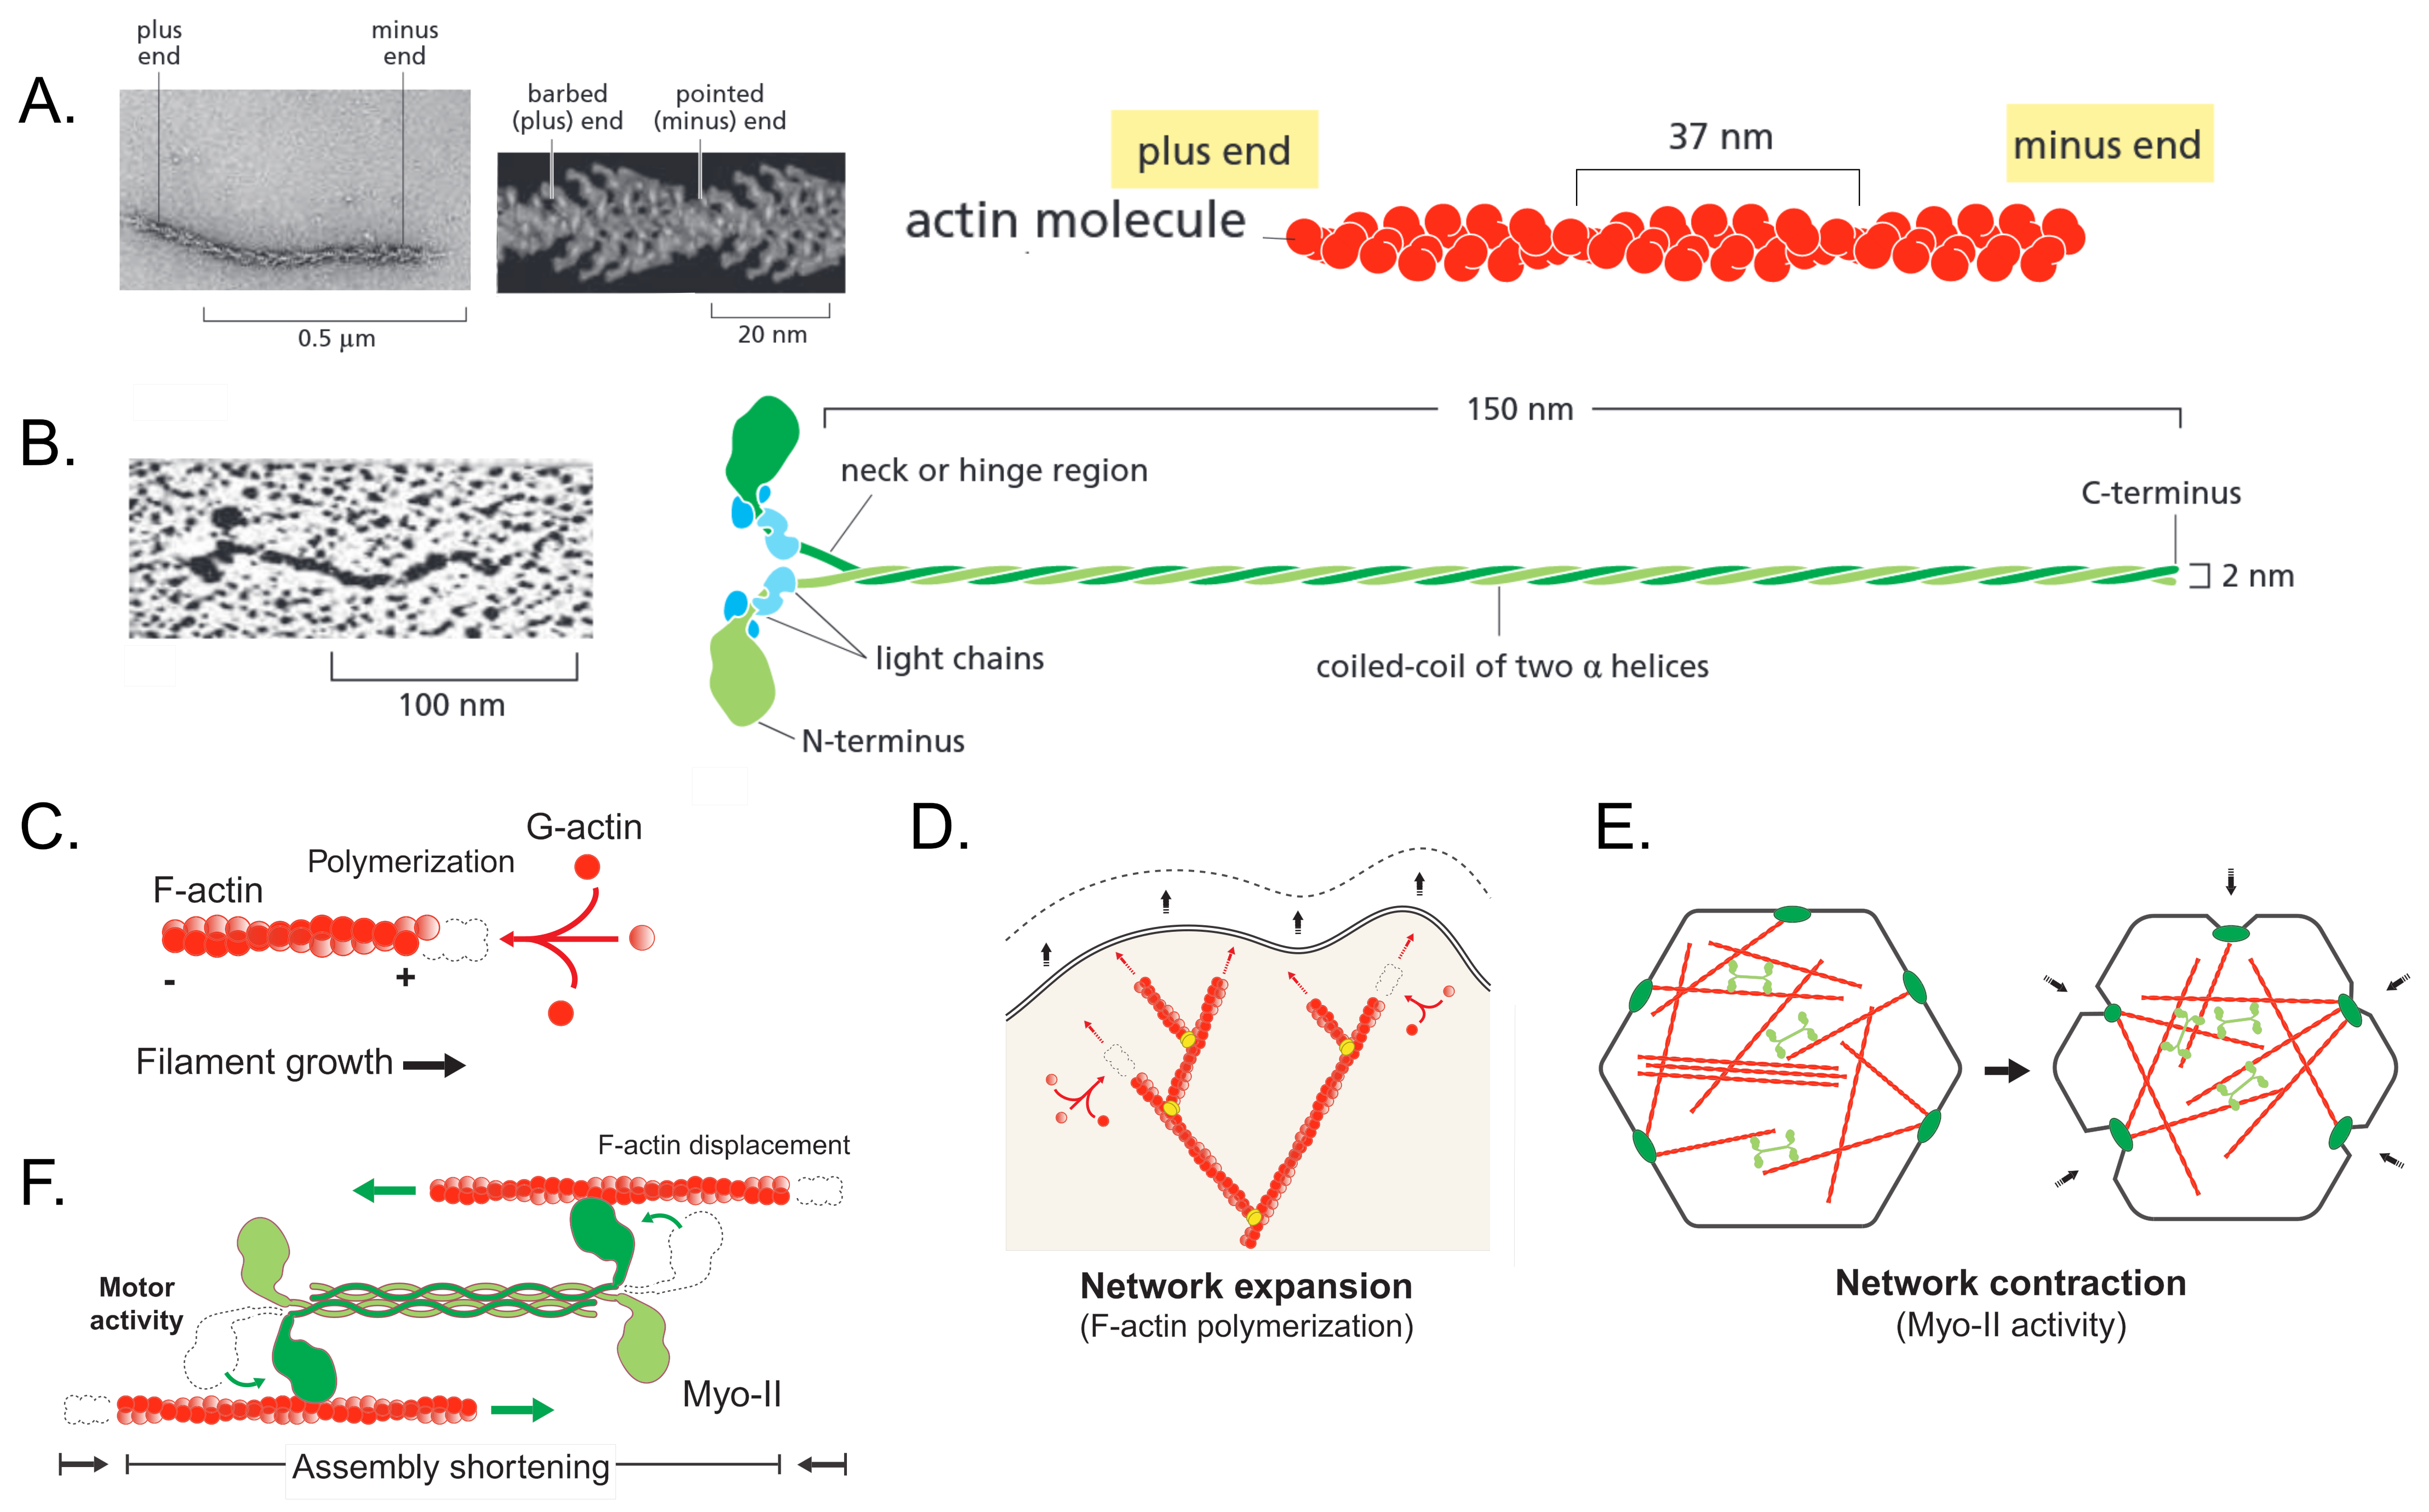
\includegraphics[width=\textwidth]{chap3actinmyosin.png}
	\caption{\label{fig_3_1} \textbf{Actin and Myosin}: (A) Electron micrograph of Actin filament with zoomed in images of barbed and pointed end. (B) Same for Myosin II minifilament with clearly visible two globular heads and a long tail. (C-D) Actin network can apply pushing force through polymerization of single filaments or network expansion. (E,F) While myosin activity would lead to contraction of the networks. \textit{Adapted from A-B \cite{alberts2015} and C-F \cite{clarke2021}}
	}
\end{figure}

\hypertarget{actin-networks}{%
	\subsection{Actin networks}\label{actin-networks}}

\begin{figure}[b!]
	\centering
	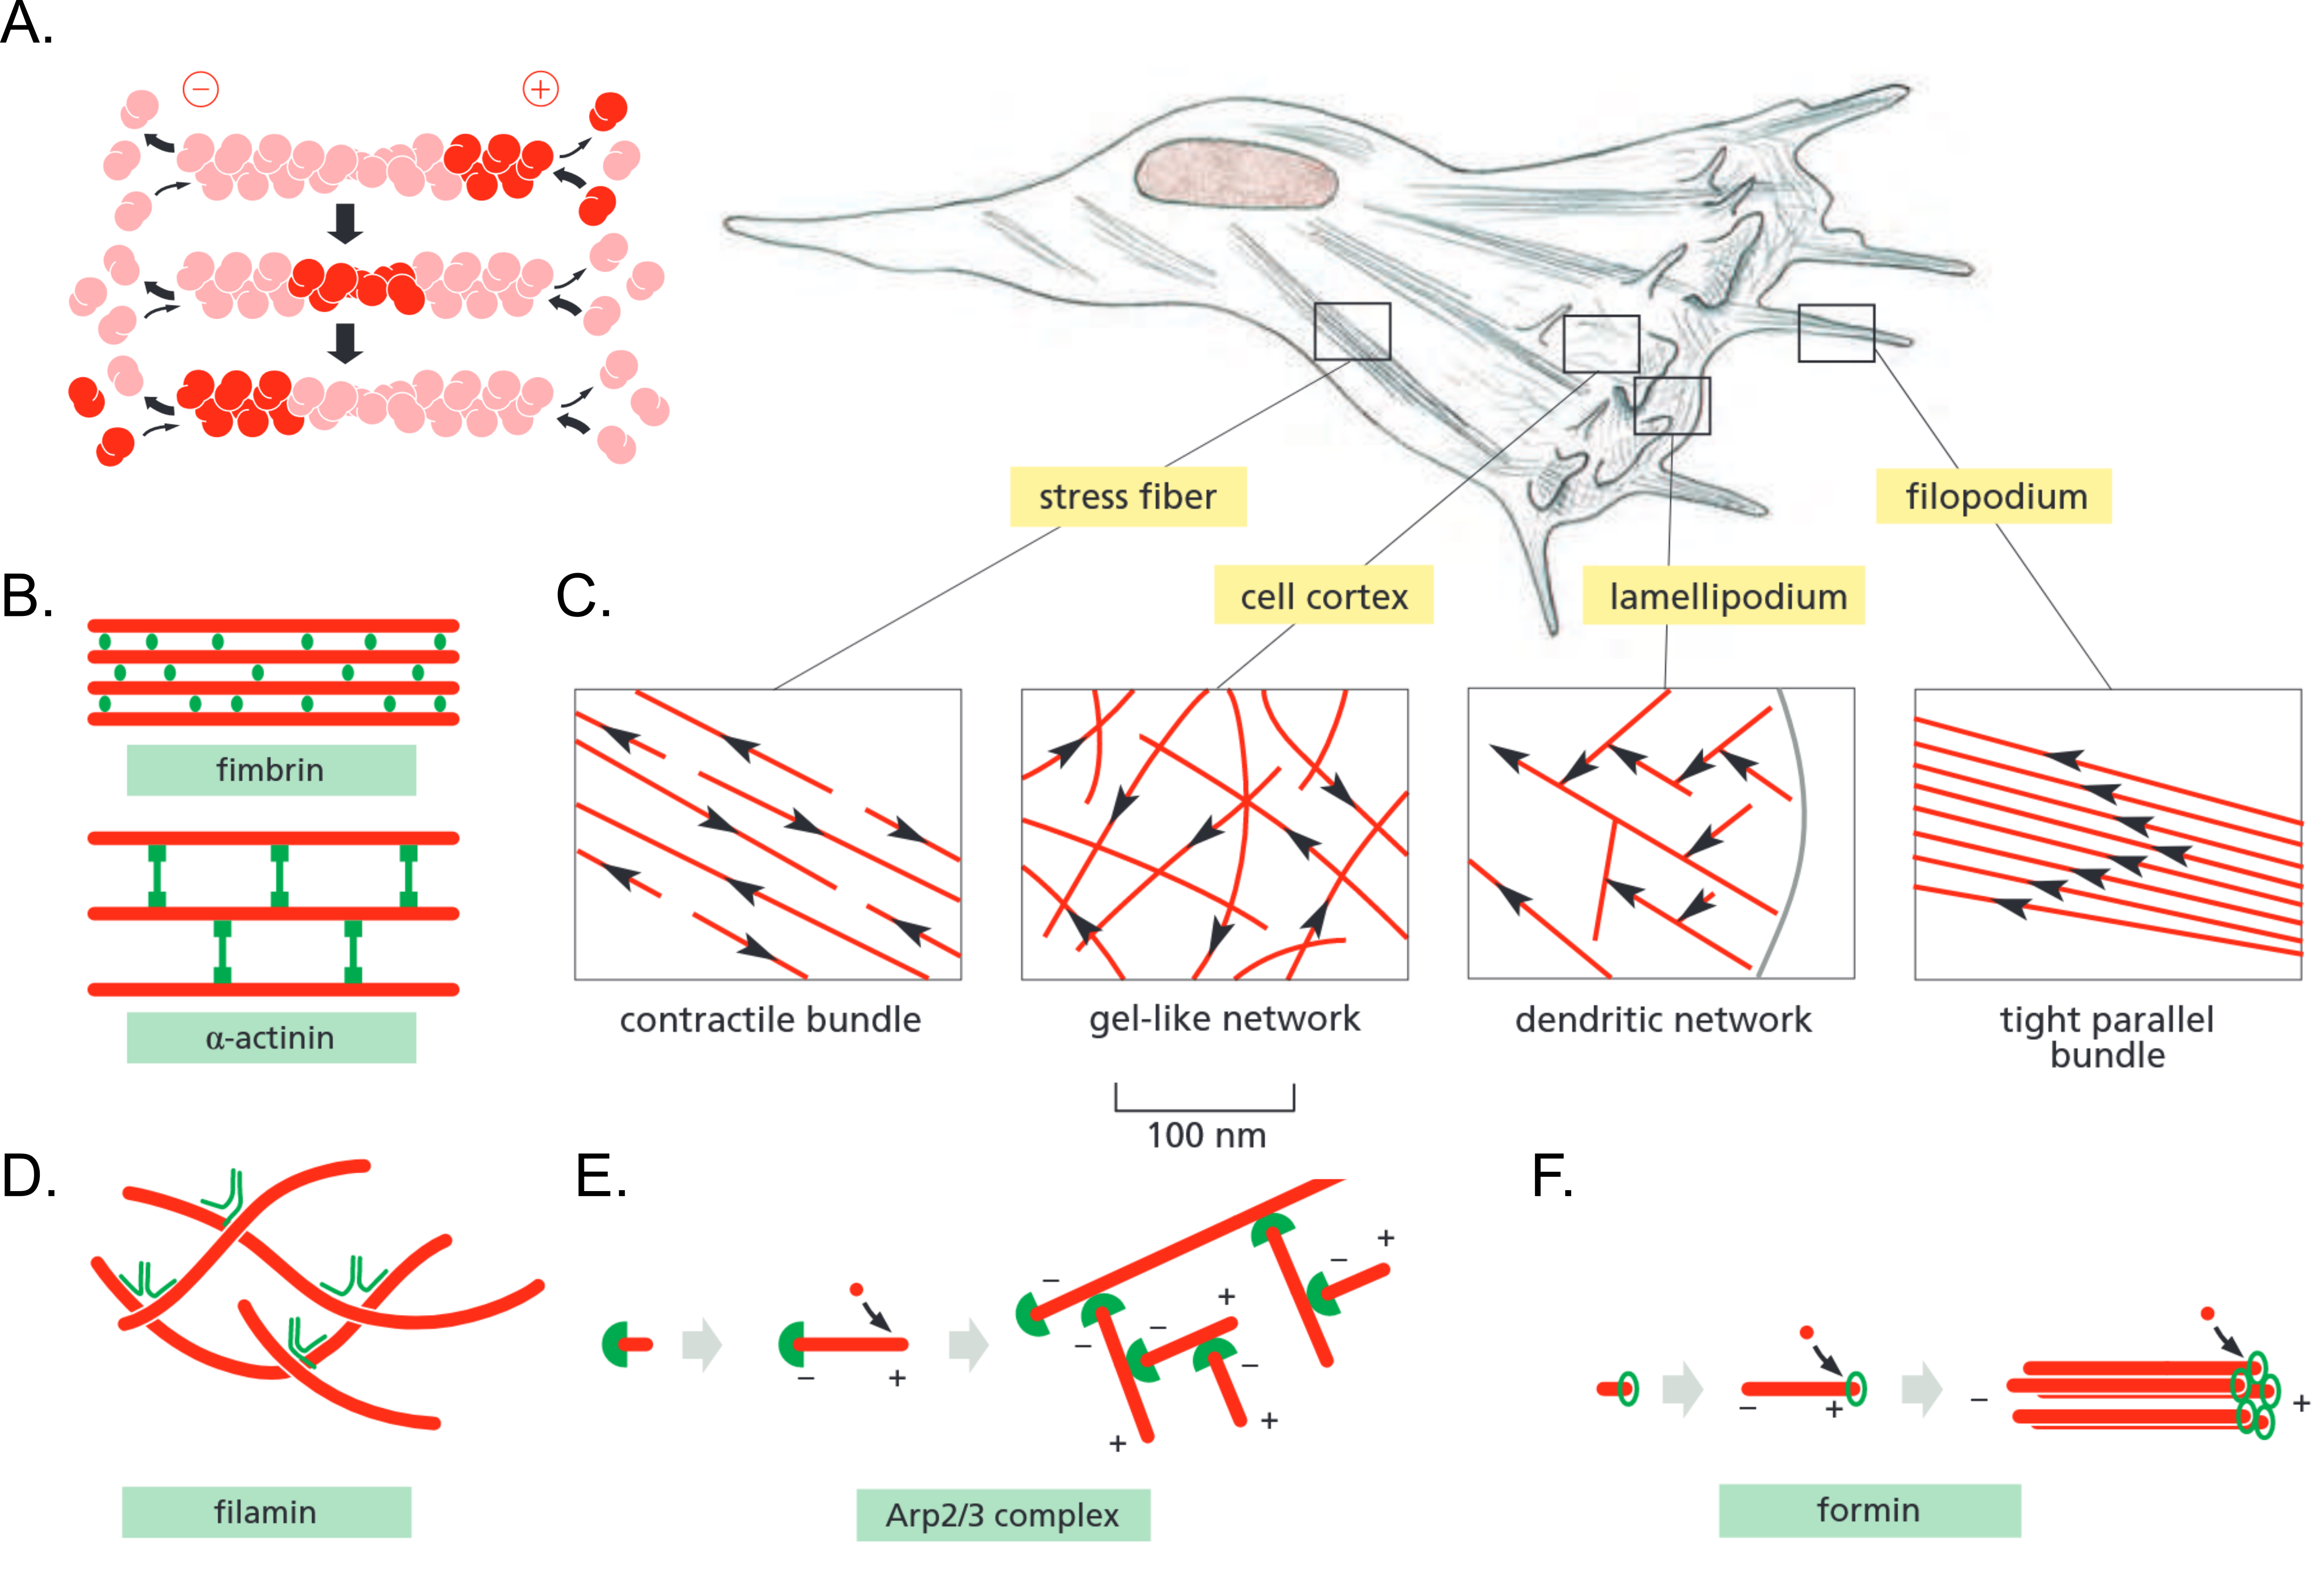
\includegraphics[width=\textwidth]{chap3actinstructures.png}
	\caption{\label{fig_3_2} \textbf{Forms of actin networks}: (A) Actin treadmilling: where highlighted actins move from positive end to negative end as the filament polymerizes and depolymerizes from both ends. (C) In an adherent cells, there are many different kinds of actin structures from contractile network to gel-like cortex. (B,D,E,F) Actin structures can be thought as meshwork of actin filaments (red) with crosslinkers(green). Different crosslinkers produce distinct form of actin network.  \textit{Adapted from \cite{alberts2015}}
	}
\end{figure}

Actin filaments can also form branched networks, facilitated by the presence of nucleation sites on the filament and proteins containing actin-binding motifs. The actin nucleation can be catalyzed by two primary factors, the ARP 2/3 complex or formins. The ARP 2/3 complex creates a pointed end in the center of a filament, leading to the formation of a new branch from that site. This results in the formation of a tree-like network of branches, capable of generating sufficient pushing forces to move a part of the cell membrane (see fig \ref{fig_3_2} E,F). The formins, in conjunction with profilin, aid in the growth of the filaments, with profilin serving as a staging area for the rapid addition of monomers to the filament. These structures can take the form of dendritic actin networks that enable membrane protrusion at lamellipodia or spike-like projections of the plasma membrane that allow a cell to explore its environment (see fig \ref{fig_3_2} C). The pushing forces generated at the molecular level are of the order of 1 piconewton.


\hypertarget{actin-cortex}{%
	\subsection{Actin cortex}\label{actin-cortex}}

The actin filaments can also form tight or loose bundles, facilitated by crosslinking proteins. Fimbrins enable multiple actin filaments to arrange in parallel, resulting in closely packed bundles that exclude myosin from connecting to the filaments. On the other hand, $\alpha$-actinin crosslinks actin filaments with opposite polarity into a loose bundle, allowing myosin to bind and create contractile bundles (see fig \ref{fig_3_2} B). Myosin II oligomerizes into a bipolar short filament that can connect multiple actin filaments and move across them, resulting in a pulling effect (see fig \ref{fig_3_1} B). This movement is driven by ATP hydrolysis making contracting an active process. The loose bundle forms the gel-like network in the cell cortex. Other actin crosslinking proteins can result in different structures. Filamin creates a loose and viscous gel that is essential for migration, while spectrin creates a strong and flexible web-like network of short actin filaments that allows cells to reversibly deform (see fig \ref{fig_3_2} D). The actomyosin bundles in the cortex can generate two orders of magnitude more force than a single filament \cite{clarke2021}.


\hypertarget{actin-structures-at-a-larger-scale}{%
\section{Actin structures at a larger scale}\label{actin-structures-at-a-larger-scale}}

During epithelial morphogenesis, individual cells can undergo shape changes by modifying their contractility or actin turnover, resulting in the development of tissue curvature. As mentioned previously, epithelial cells exhibit apicobasal polarity, which results in a non-uniform distribution of the actin cytoskeleton that influences cell shape and tissue architecture.

The geometry of columnar or wedge-like cells in a monolayer determines the specific ways in which they can be organized \cite{gomez-galvez2021}. Columnar cells, when arranged together, produce a flat tissue, while wedge-shaped cells with a narrow top result in convex curvature (see fig \ref{fig_3_4} A ). Conversely, concave curvature with a narrow bottom can also be created. By observing the actin cytoskeleton, we can determine the specific mechanisms of tissue shaping (see fig \ref{fig_3_4} B). For example, apical constriction with concentrated actin cortex on the apical surface is involved in multiple convexly curved tissues, such as the invagination of the intestinal crypt, the Drosophila mesoderm, and the vertebrate lens placode \cite{perez-gonzalez2021, lecuit2011, houssin2020}.

\begin{figure}
	\centering
	\includegraphics[width=\textwidth]{chap3realactin.png}
	\caption{\label{fig_3_3} \textbf{Actin organization at different scales}:(A) Electron micrograph of actin cortex of mitotic Hela cells \cite{kelkar2020}. (B) Different forms of actin organization in circular fibroblast cell \cite{jalal2019} Scale$= 10\mu m$. (C) Supracellular actin ring during wound closure \cite{brugues2014} Scale$=20 \mu m$. (D) Dorsal closure of amnioserosa with actin network \cite{ducuing2016} Scale$= 10 \mu m$. (E) Supra-cellular organization of actin for cellularization of coenocyte. Circle is $60 \mu m$ \cite{dudin2019}. (F) Hydra with actin network, whose nematic defects determines morphogenesis \cite{maroudas-sacks2021} Scale$= 100 \mu m$.
	}
\end{figure}

On the other hand, basal constriction results in opposite curvature, as observed in the optic cup and mid-hind brain fold of zebrafish \cite{sidhaye2017, gutzman2018}. However, convex curvature can also be produced through basal expansion, as seen in the Drosophila wing disc (see fig \ref{fig_3_4} A). Certain parts of the wing disc can locally relax the basal side without affecting the apical side, leading to basal expansion \cite{sui2018}. In addition to the apical and basal surfaces, lateral surfaces can also contract or expand due to myosin II activity, which can cause tissue folding in the wing and leg discs of Drosophila \cite{sui2018, monier2015}. Furthermore, cell-cell rearrangements can be produced by altering junction lengths during germ band extension \cite{yu2016, collinet2015} (see fig \ref{fig_3_4} C). 

Not only do individual cells undergo coordinated actin reorganization during epithelial morphogenesis, but supracellular actin structures can also emerge at the tissue level (see fig \ref{fig_3_3} A-C). Junctional actomyosin organizes to form bundles connected across multiple cells, allowing for important functions such as wound healing and morphogenesis \cite{brugues2014, clarke2021} (see fig \ref{fig_3_4} D-F). These supracellular networks can exert forces at the scale of the embryo, as observed in cases such as dorsal closure and parasegment boundary formation in Drosophila and epiboly in zebrafish \cite{ducuing2016, calzolari2014}. Additionally, these networks can alter the material properties of specific regions in the embryo, making them more prone to deformation and thus aiding in the formation of folds or invaginations (see fig \ref{fig_3_4} G). 

During Drosophila gastrulation, tissue-level actin cortex is altered in the direction of the anterior-posterior axis, providing increased bending strength in that direction. This supports the internalization of the mesoderm by promoting folding in a perpendicular direction \cite{yevick2019}. Interestingly, highly organized actin bundles are also found in even larger systems such as Hydra, vertebrate smooth muscle, and the heart \cite{maroudas-sacks2021, palmer2021, cetera2014, helm2005} (see fig \ref{fig_3_3} D-F). These bundles assist in generating mechanical force patterns that create coordinated tissue movements at a global scale.


\begin{figure}
	\centering
	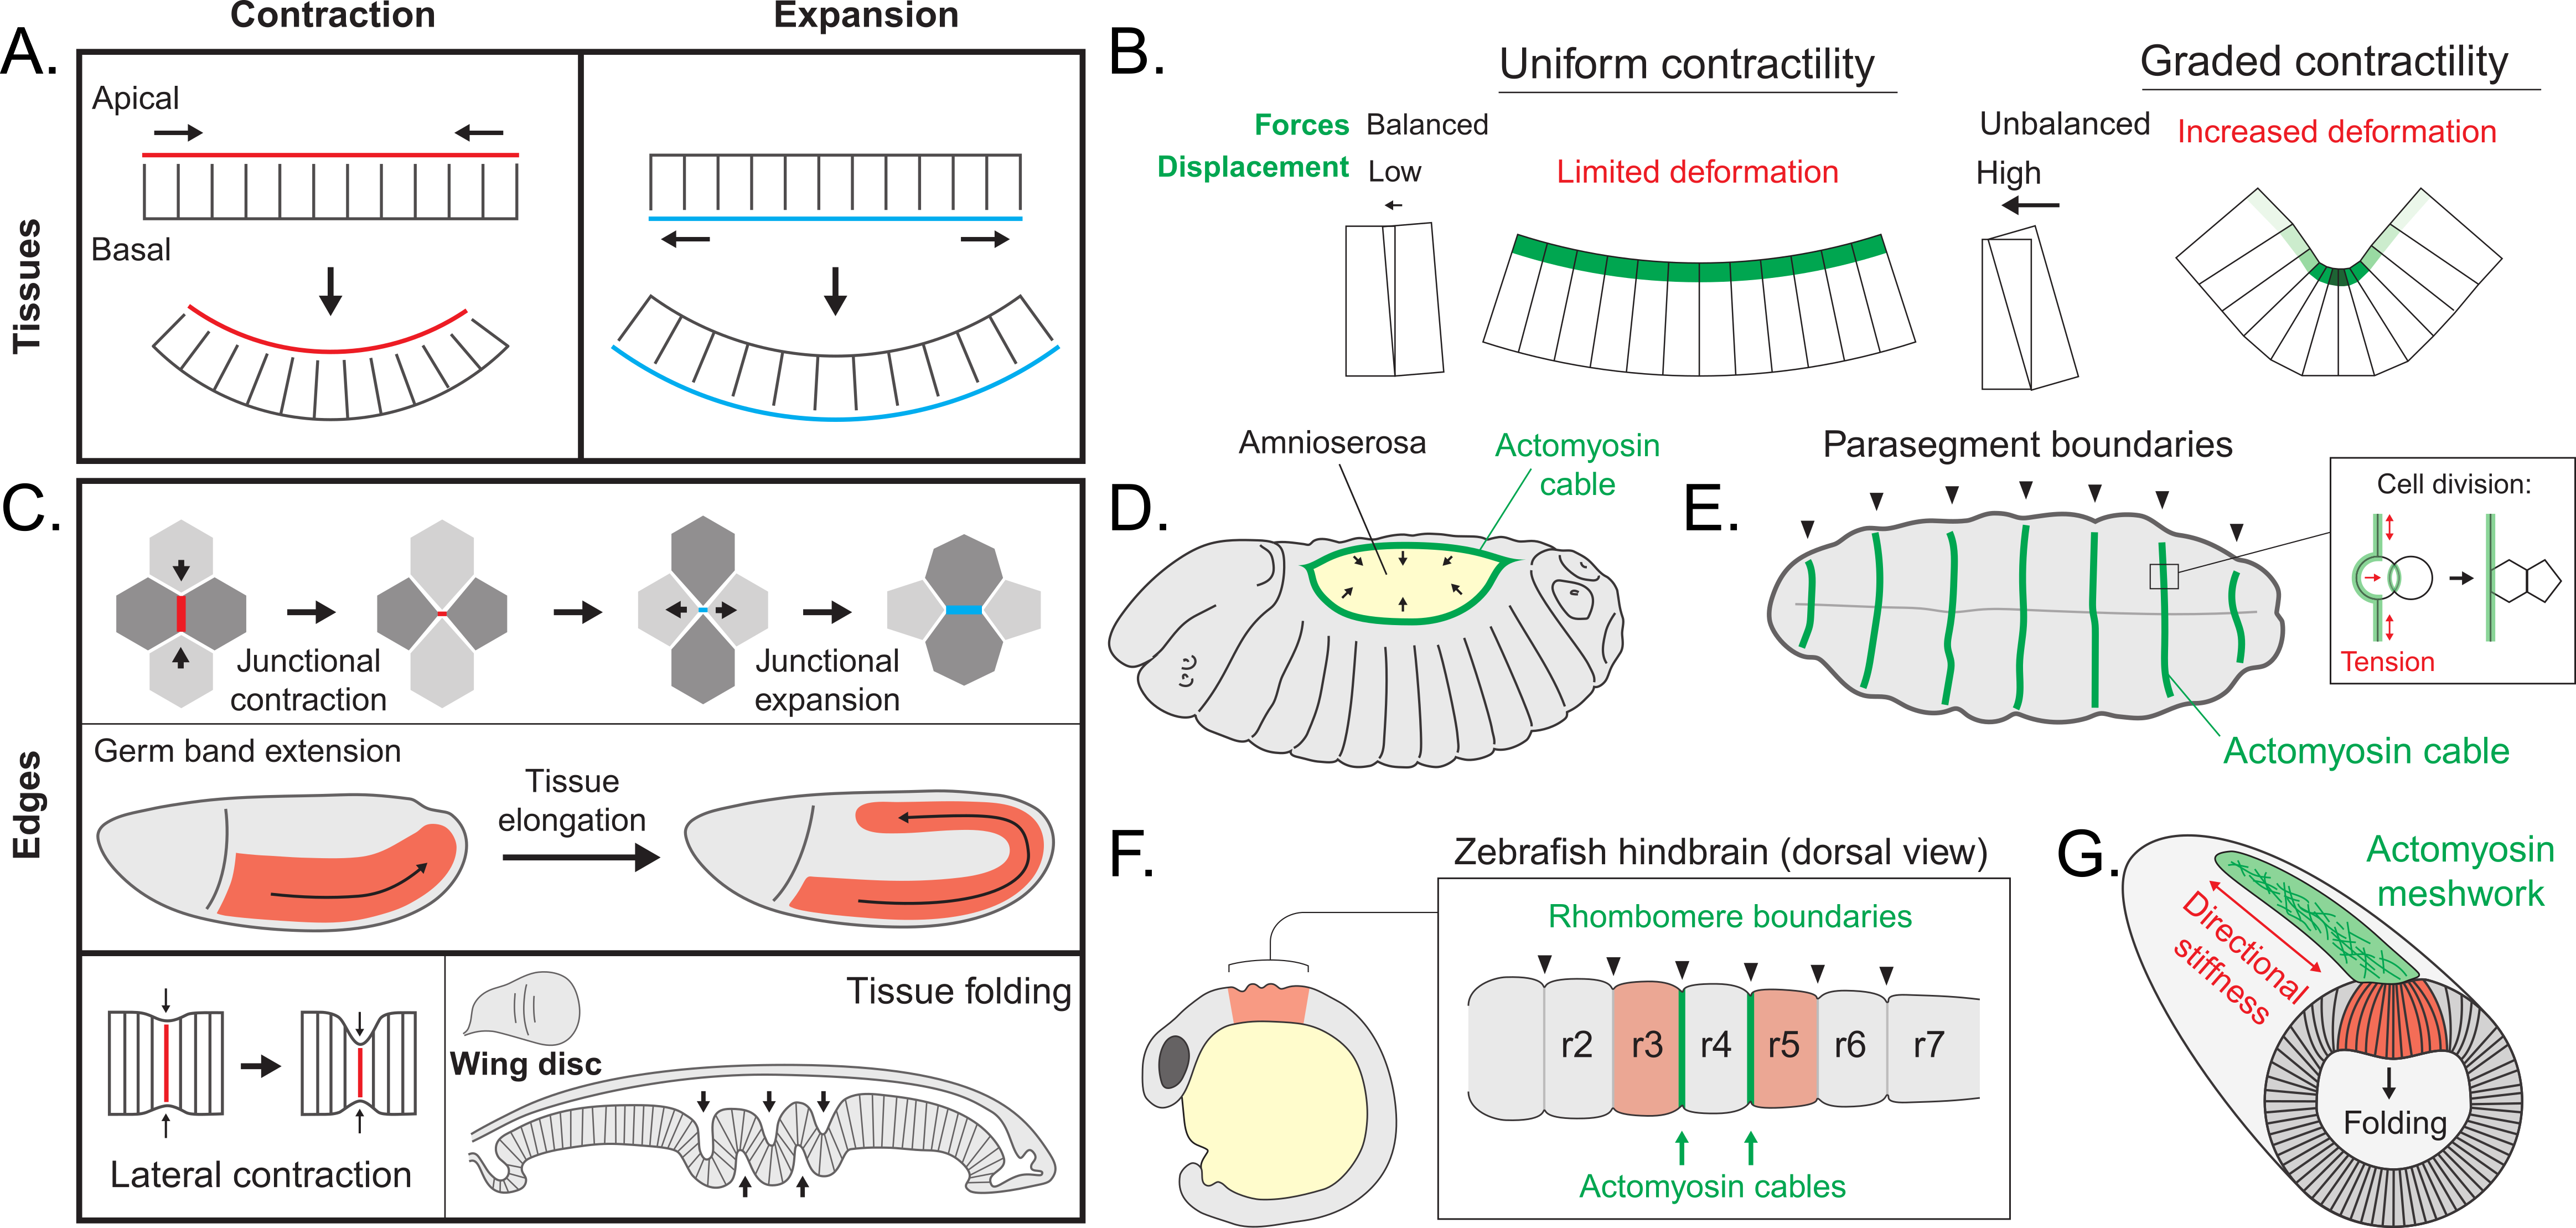
\includegraphics[width=\textwidth]{chap3actinsuper.png}
	\caption{\label{fig_3_4} \textbf{Morphogenesis driven by actin at tissue scale}: (A) Apical contraction or basal relaxation both results in the same curvature. (B) However, amount of deformation will depend on the contractility gradient. (C) Lateral surface of cells can also undergo expansion or contraction leading to cell rearrangements or tissue folding. (D-G) Supracellular actin cables plays vital role in creating boundaries or causing large scale deformations. \textit{Adapted from \cite{clarke2021}}
	}
\end{figure}

\hypertarget{timescales-of-the-actin-cytoskeleton}{%
	\section{Timescales of the actin
		cytoskeleton}\label{timescales-of-the-actin-cytoskeleton}}

Morphogenesis, the process of shaping and forming living structures, occurs at varying timescales and requires the cell cytoskeleton to change its shape accordingly. Rheological and mechanobiological experiments have given us insights into how cells respond to forces and deformations based on their magnitude and rate (see fig \ref{fig_3_5}; reviewed in \cite{wyatt2016}).

For fast deformations (in the range of milliseconds to seconds), cells exhibit predominantly elastic behavior, as there is insufficient time for the actin cortex to respond or remodel \cite{deng2006}. The cytoskeleton can store elastic energy and release it. At this scale, there is also flow of cytosol through the cortical mesh, resulting in poroelastic behavior\cite{moeendarbary2013}.

When forces or deformations are applied over longer timescales (seconds to minutes), cells exhibit an increasingly viscoelastic behavior \cite{kollmannsberger2011}. The actin cortex can flow and is unable to fully store energy. The actin filaments and crosslinkers, such as myosins and actinin, allow the cytoskeleton to remodel in response to mechanical perturbations through turnover in tens of seconds or a few seconds, respectively. Myosin mini filaments, however, can take longer to remodel, up to hundreds of seconds.

At even longer timescales (minutes to hours), cells or tissues may respond through oriented division or rearrangement, allowing them to adapt to persistent forces such as gravity or surface tension. Tissues may resemble a viscous fluid and morph into a sphere, such as a blastocyst. Interactions with the extracellular matrix over hours can lead to adjustments in the constitutive tension of tissues based on biophysical and biochemical forces \cite{porazinski2015}.

\begin{figure}
	\centering
	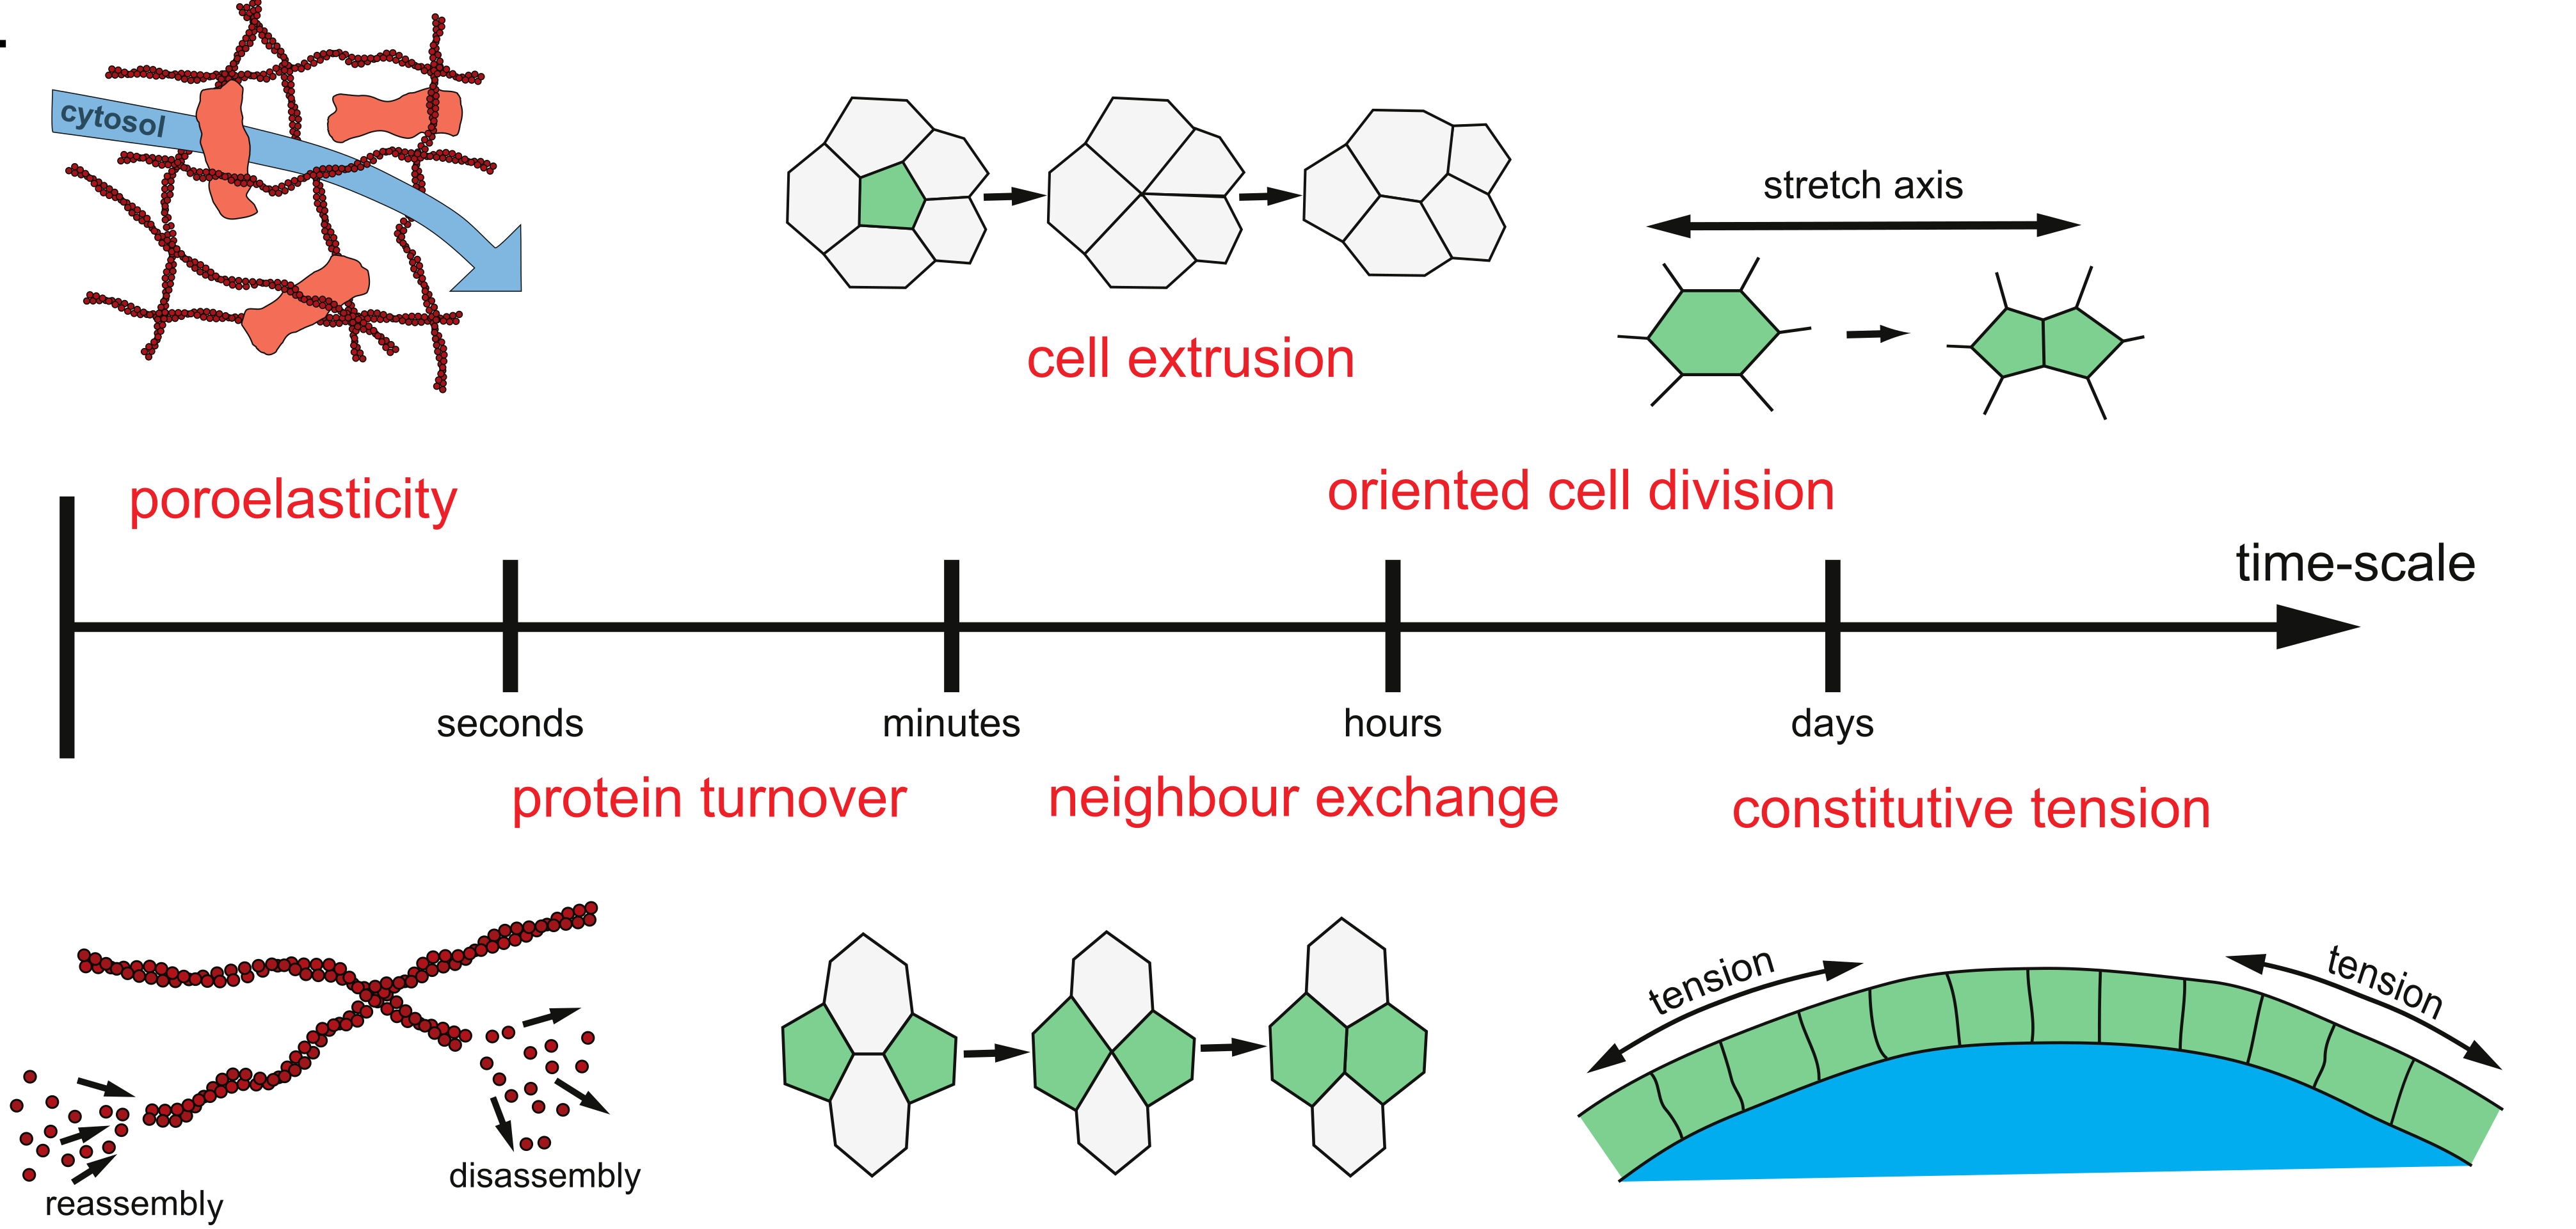
\includegraphics[width=\textwidth]{chap3timeactin2.png}
	\caption{\label{fig_3_5} 
		\textbf{Timescale of actin network related processes}: Timescales of different actin driven cellular processes, ranging from cytoskeletal fluid deformation to large-scale tissue deformations. \textit{Adapted from \cite{kelkar2020}}.}
		%\textbf{Molecular pathway and timescale of actin network related processes}: (A) Timescales of different actin driven cellular processes, ranging from cytoskeletal fluid deformation to large-scale tissue deformations. (B) Molecular signaling of RhoGTPase. RhoGEFs return GDP for GTP to activate RhoA. In turn RhoA results in actomyosin contractility. \textit{Adapted from \cite{kelkar2020, wyatt2016}}.
\end{figure}

%\hypertarget{controlling-cortical-tension}{%
%	\section{Controlling cortical
%		tension}\label{controlling-cortical-tension}}
%
%The magnitude of contractile or tensile forces exerted by cells is greatly influenced by the tissue type and its environment. The signaling pathways regulating the crosslinkers and nucleators of actin bundles are responsive to both external biochemical and biomechanical stimuli (see fig \ref{fig_3_5} B; reviewed by \cite{kelkar2020}). The actomyosin bundles, made up of dynamic actin filaments, constantly undergo cycles of contraction, polymerization, and depolymerization, which maintain a homeostatic level of cortical tension in healthy tissues. As a result of the numerous components involved in the actin network, cortical tension can be readily modulated by pharmacological interventions targeting specific molecular targets \cite{cartagena-rivera2016}.
%
%For example, the use of Latrunculin, which binds to actin monomers, can result in the depolymerization of the actin network and reduce contractility. Similarly, inhibiting myosin activity with Blebbistatin leads to a decrease in cortical tension due to its hindrance of myosin II ATPase activity. Conversely, Calyculin-A enhances contractility by accelerating the rate of Myosin II phosphorylation. The stability of the actin network can also be impacted by sequestering ARP 2/3 monomers with CK666, which increases cortical tension. Other factors, such as Rho-GTPases and calcium levels, located further along the signaling pathway, can also affect network stability \cite{valon2017}.
%
%Optogenetic tools offer a more refined and localized means of controlling contractility. For instance, tools based on the regulation of RhoA can be used to locally regulate cell protrusion, tissue tension, and traction \cite{valon2017}. A recently developed tool controlling Shroom3 provides even finer control over apical constriction and can be used to recreate tissue folding \cite{martinez-ara2022}.

\hypertarget{modeling-active-tissue-dynamics}{%
	\section{Modeling active tissue
		dynamics}\label{modeling-active-tissue-dynamics}}

The advancement of molecular biology and tissue dynamics has increased our understanding of morphogenesis. However, it is becoming increasingly crucial to interpret biological experiments through theoretical models in order to generate new hypotheses and validate them through further experimentation.

Mathematical models at multiple scales are used to describe both physics and biology. At larger tissue scales, hyperelastic continuum material models could be utilized to describe the behavior of the cardiovascular system \cite{holzapfel2019}. On smaller scales, agent-based models are used to explain epithelial tissue behavior in terms of cell sorting and reorganization \cite{voss-bohme2012}. This section aims to provide the reader with a brief overview of the relevant modeling approaches in this field.

\begin{figure}
	\centering
	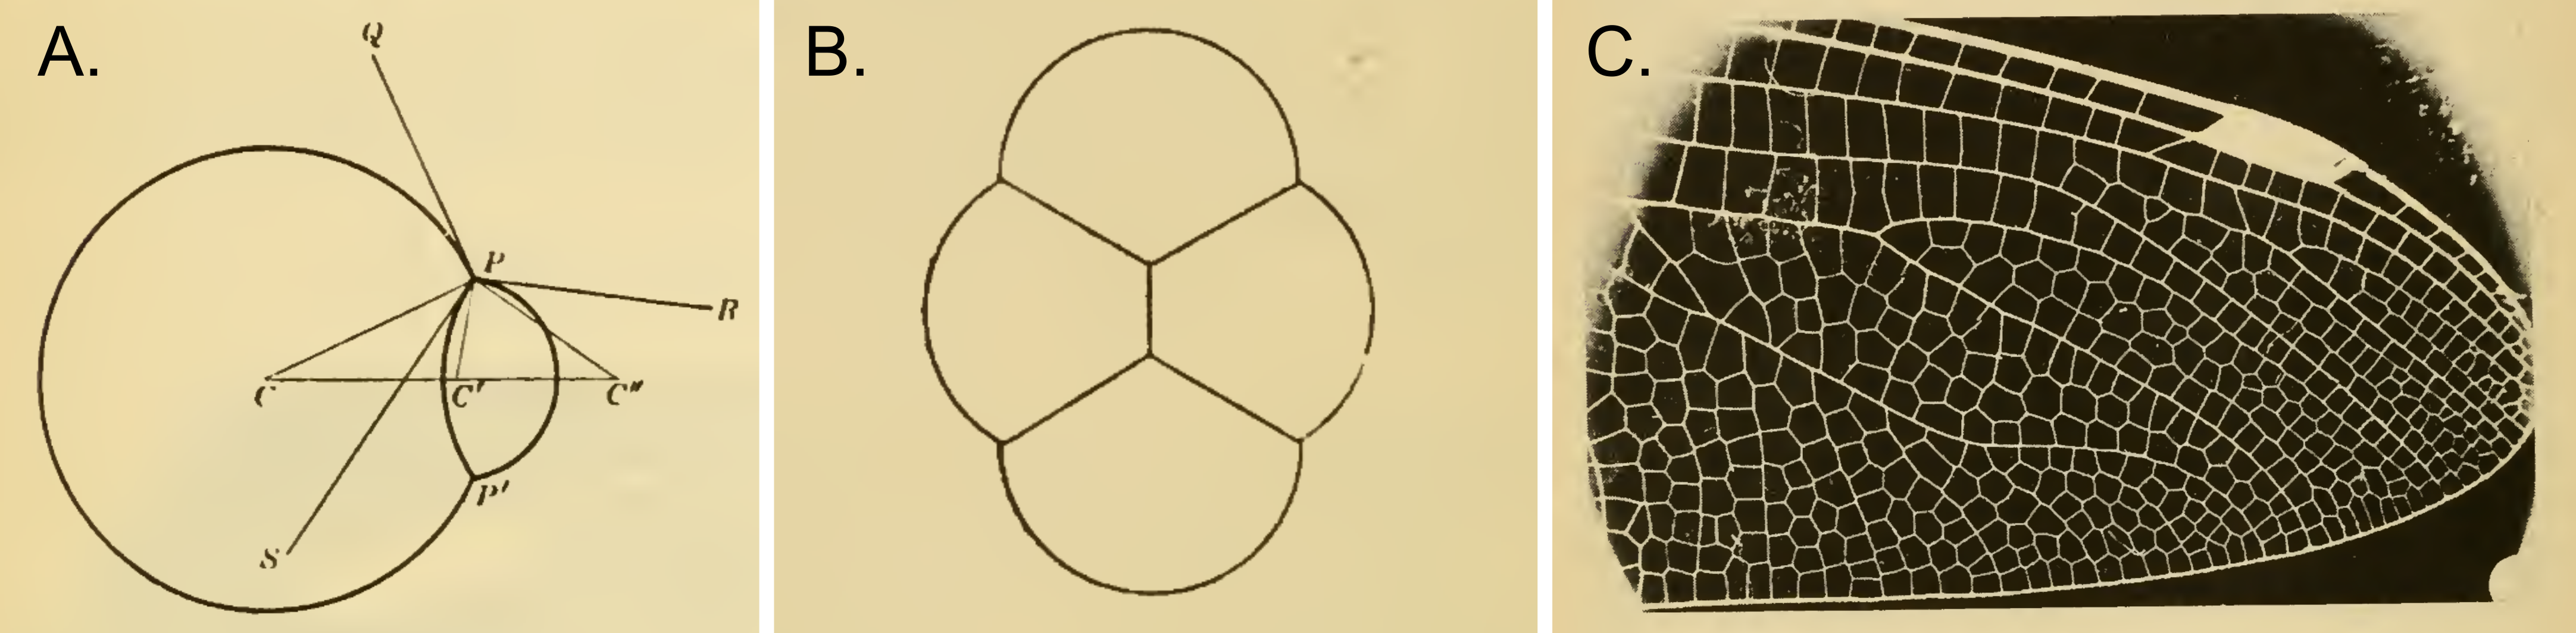
\includegraphics[width=\textwidth]{chap3darcy.png}
	\caption{\label{fig_3_6} \textbf{D'Arcy Thompson's forms of tissues:} (A-B) Thompson equates cell aggregates to coalescence of bubbles like in a froth. (C) A dragon fly wing is a clear example of this organization. \textit{Adapted from \cite{thompson1979}}
	}
\end{figure}

\hypertarget{vertex-models}{%
	\subsection{Vertex models}\label{vertex-models}}

D'Arcy Thompson, in his chapter on ``The Forms of Tissues,'' presents an intuitive argument regarding the role of surface tension or capillarity in organizing cells into a tissue \cite{thompson1979, graner2017}. He observed this phenomenon in a wide range of biological systems, from two connected cells to the organization of cells in a dragonfly wing, which resemble the
associations of soap bubbles or foams (see fig \ref{fig_3_6}).
\footnote{"we recognize the appearance of a "froth," precisely resembling that which we can construct by imprisoning a mass of soap-bubbles in a narrow vessel with flat sides of glass; in both cases we see the cell-walls everywhere meeting, by threes, at angles of $120 \deg$, irrespective of the size of the individual cells: whose relative size, on the other hand, determines the curvature of the partition-walls", writes Thompson}
In the case of monolayered epithelial tissue, its polygonal cellular pattern on its surface enables the easy description and tracking of cell motion and shape change through the use of vertices and edges.
\begin{wrapfigure}{r}{5.5cm}
	\caption{\textbf{Vertex model for cells in a monolayer} \textit{Adapted from \cite{gomez-gonzalez2020}}.}\label{fig_3_7}
	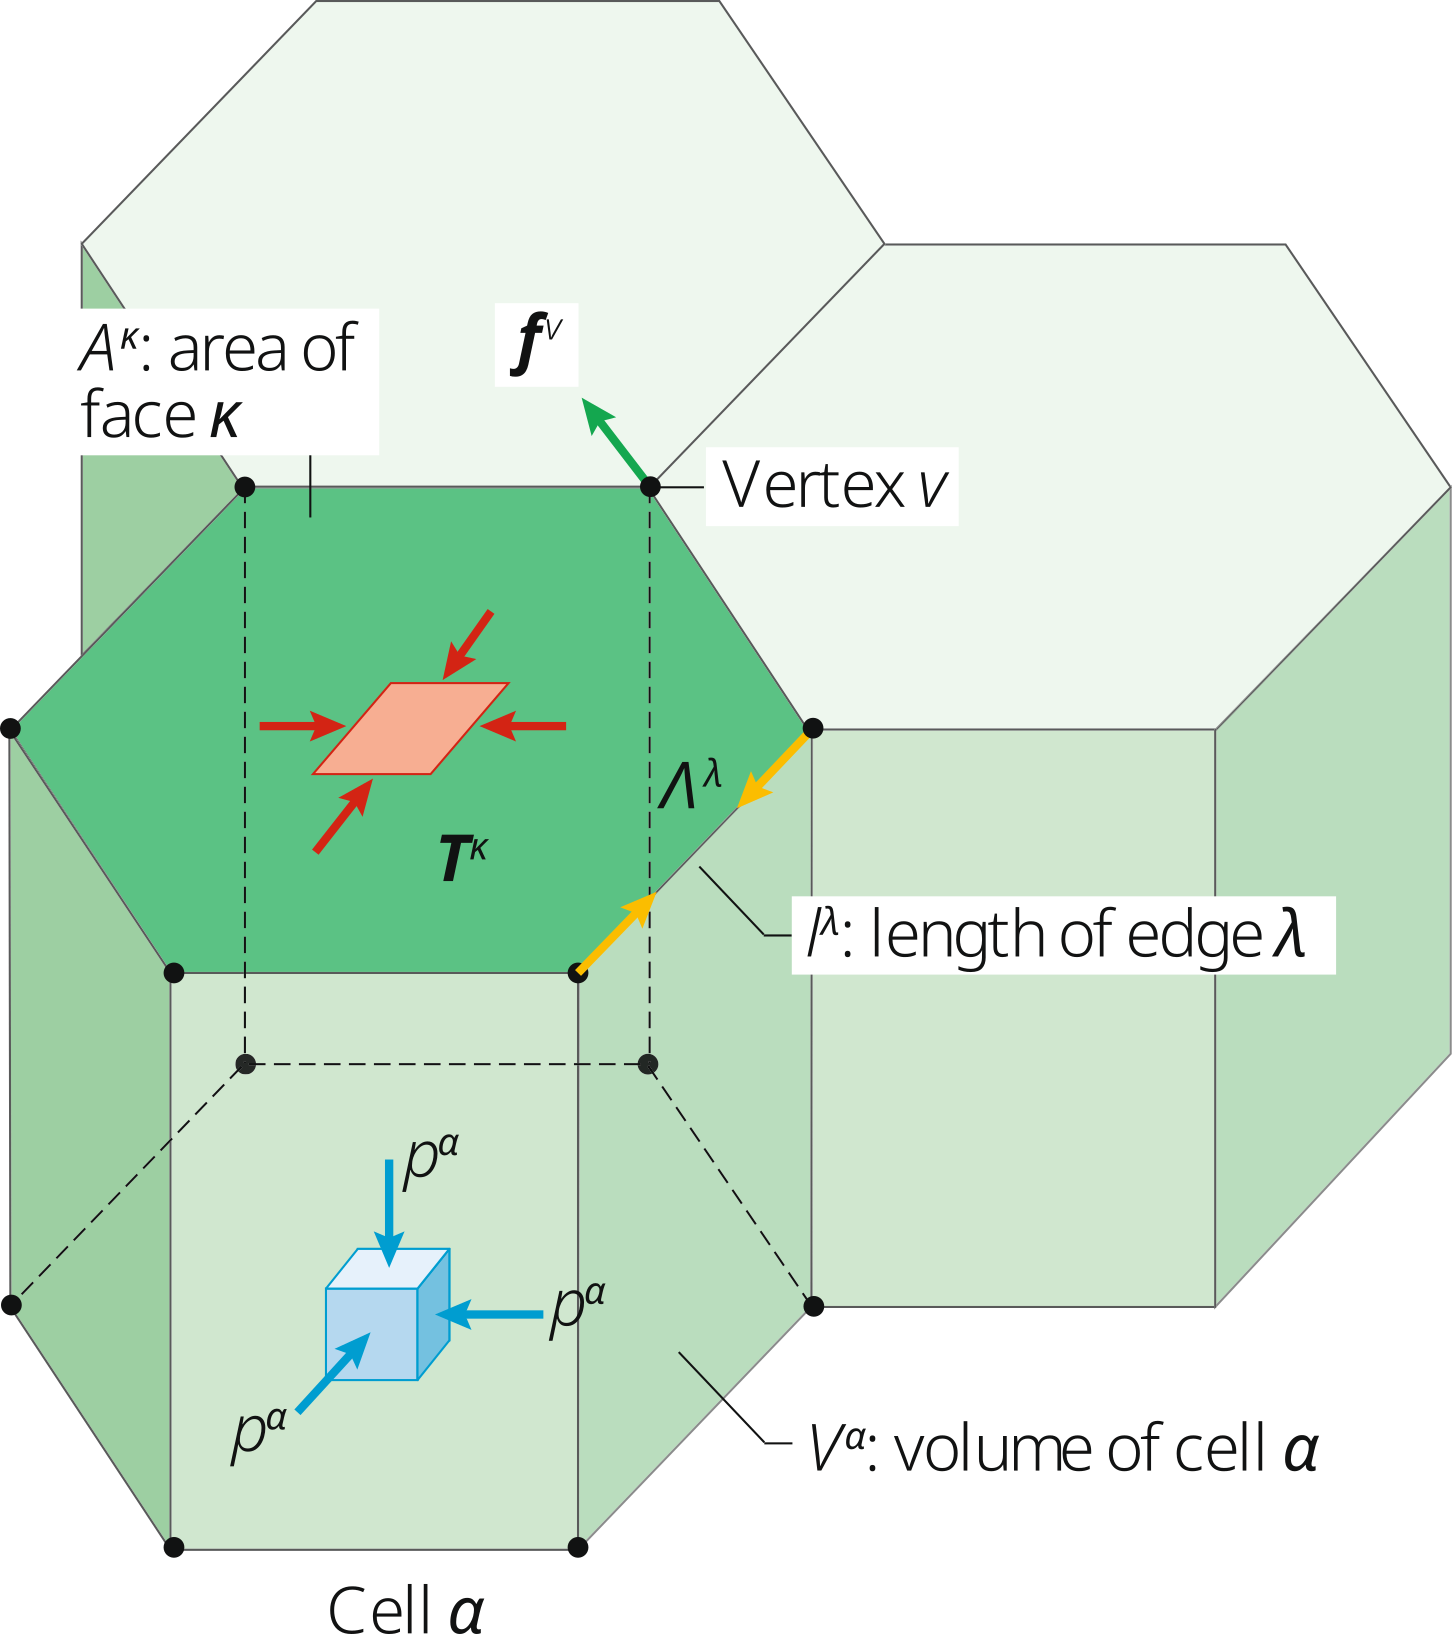
\includegraphics[width=5.5cm]{chap3vertex.png}
\end{wrapfigure} 
Vertex models have proven to be valuable in understanding the complex interactions between cellular shape, the forces generated within epithelial cells, and the mechanical constraints imposed on the tissue from external sources (as reviewed in \cite{alt2017}). These models can be two-dimensional or three-dimensional, depending on the system being modeled, but cells are consistently defined as having both an apical and basal surface, as well as lateral interfaces between neighbors. Further complexities have been added to describe specific systems, such as intercalations in three-dimensional epithelia, through the use of a geometric shape known as the Scutoid (reviewed in \cite{gomez-galvez2021}).

To determine the motion of the vertex, mechanics must be specified. It is often done using the virtual work function (W). There are two components: internal $(\delta W_i)$ and external $(\delta W_e)$. 
$$ \delta W = \delta W_i + \delta W_e .$$ 
The changes in internal virtual work,  $(\delta W_i)$ can result from changes in the cell volumes $(\delta V)$, in the areas of surfaces $(\delta A)$, or in the lengths of bonds $(\delta l)$. By defining the cell pressure $(P)$, the surface tension $(T)$, the line tensions $(\Lambda)$, and internal dissipative forces $(f_i)$, the differential of the internal virtual work for vertex movements can be written. 
$$ \delta W_i = \Sigma_{cell\ \alpha} \left( -P^\alpha \delta V^\alpha \right) + \Sigma_{surface\ k} \left( T^k \delta A^k \right) + \Sigma_{edge\ \lambda} \left( \Lambda^\lambda \delta l^\lambda \right) - \Sigma_{vertex\ \nu} \left( f_i^\nu \delta x^\nu \right). $$
Similarly, the external virtual work, $(\delta W_e)$, can be written according to the external forces $(f_e)$ that come from external mechanical forces applied to the tissue through the matrix, or fluid pressure acting on apical or basal cell surfaces.
$$ \delta W_e =  - \Sigma_{vertex\ \nu} \left( f_e^\nu \delta x^\nu \right). $$
The state of a monolayer is determined by minimizing the virtual work function, taking into account the molecular complexities that contribute to surface tension and line tensions. In the context of epithelial layers, the actin cortex significantly impacts the tensions along the edges. Vertex model simulations in 2D models demonstrate the important role of interfacial tensions in shaping cell orientation, coordinating collective migration, and facilitating tissue rearrangement through cell division.

In contrast, 3D models capture the physics of various morphogenetic processes, such as the formation of appendages on the drosophila eggshell and the mechanical compartmentalization of intestinal epithelia \cite{osterfield2017, perez-gonzalez2021}. These models offer unique insights into cell packing and the transition between jamming and unjamming \cite{park2015, tang2022}. In some cases, phase transitions from a solid to fluid state result from localized proliferation and oriented divisions, showing that the epithelial tissue behaves as an active material (reviewed in \cite{lenne2022}).

\hypertarget{continuum-models}{%
	\subsection{Continuum models}\label{continuum-models}}

The viscoelastic properties of tissues are captured in vertex models, which are useful for smaller scale. However, for larger scale deformations or flows, we can model tissues as a continuous material. There are two tactics for thinking about these models: one focuses on the rheological properties of the tissue, and the other on shape transformations. By thinking of a continuous sheet of cells as an active surface, we can capture the physics of single cells to embryos \cite{salbreux2017, khoromskaia2023}.

Continuum models focus on developing reliable constitutive relations and solving initial-boundary-value problems. Constitutive relations describe how materials respond to applied loads, and they depend on the internal constitution of the material. Determining constitutive relations for epithelial monolayers can be challenging because these tissues are much more complex than simple metals or passive polymers (see fig \ref{fig_3_8} A-B). However, their complex material behavior can be understood by characterizing their mechanical response using standard material testing techniques \cite{humphrey2002}. Typically, they can be probed mechanically in a biologically relevant manner, such as through biaxial or uniaxial stretching experiments that simulate \textit{in vivo} tissue behavior \cite{humphrey2014}. These experiments with epithelial tissues have revealed the viscoelastic nature of these materials \cite{harris2012, khalilgharibi2019}.

Solids, such as rubber, are considered to have elastic properties, allowing them to deform reversibly when subjected to a force. Conversely, fluids are characterized by their viscosity, meaning they flow in response to an applied force. Viscoelastic materials exhibit both solid-like and fluid-like behaviors (see fig \ref{fig_3_8} C). Simple models can represent these behaviors by combining elastic components, represented as springs, and viscous components, represented as dashpots. The elastic response does not dissipate energy, unlike the viscous response. $$ \sigma = E\epsilon ,\ \ \ \ \sigma = \eta \frac{d\gamma}{dt}. $$ Other material properties like stiffness or Poisson's ratio can be revealed through quasi-static stretching or compression. However, dynamic properties are better understood through frequency sweep, creep, or stress relaxation experiments \cite{guimaraes2020}. Rheological experiments have been extremely valuable in gaining insight into the mechanical response of various biological materials, ranging from reconstituted cytoskeletal proteins to large multicellular aggregates \cite{mofrad2009, cavanaugh2020, xi2018}.

Rheological properties are often linked to physiological state and are crucial for their specific functions \cite{park2015, vedula2012}. For example, many fundamental shape transitions in embryos occur through abrupt change in tissue material properties. \cite{hannezo2022}. Therefore, it is important to assess rheological properties in different microenvironments. Mechanical information such as deformation, deformation rates or velocity fields, traction forces exerted by cells on substrates, and intercellular mechanical stress can provide a more complete picture of tissue rheology when combined with information about cellular architecture obtained through imaging \cite{roca-cusachs2017}. These types of experiments shed light on the complex mechanisms of strain stiffening and viscoelastic behavior at different deformation regimes involving various parts of the cytoskeleton.

\begin{figure}
	\centering
	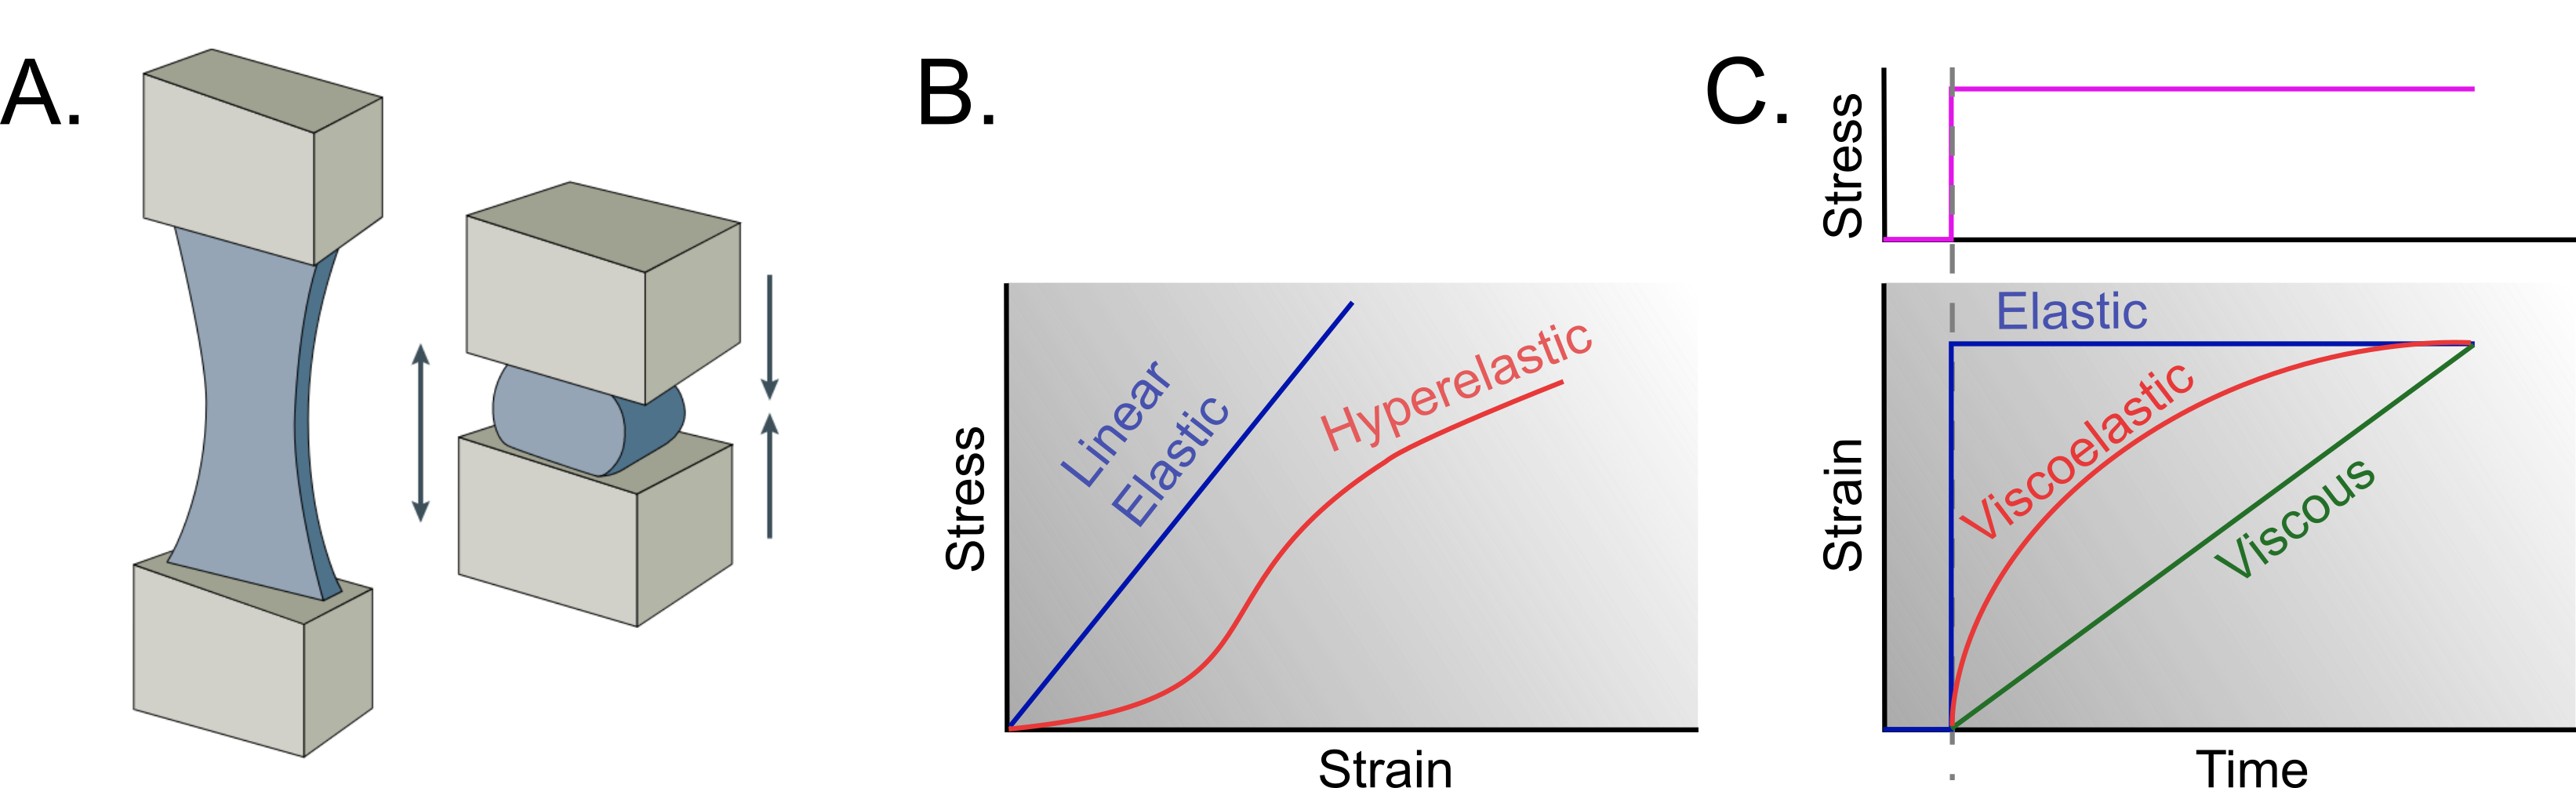
\includegraphics[width=0.85\textwidth]{chap3elastic.png}
	\caption{\label{fig_3_8} \textbf{Stress strain behavior of materials}: (A) materials being stretched or compressed. (B) Quasistatic deformations yield stress-strain curves. (C) Creep test where strain response is characterized at constant stress.
	}
\end{figure}

However, in certain cases like modeling cardiovascular mechanics or the growth of organs, we can rely on hyperelasticity or composite material framework. The basic kinematics assumes a mapping, \(x = \chi (X, t)\), deformation from reference to deformed configuration. The deformation gradient and Green's strain tensor are defined. 
$$ F = \nabla_X (\chi(X, t)));\ \ \ \ E = \frac{(F^T F - I)}{2}. $$ 
The elastic and growth can be delineated in the deformation gradient through decomposition. \[ F = F_e F_g .\] Here, in the theoretical framework of finite elasticity, one can assume a strain energy function relates to stress. The stress-strain data extracted from the experiment allows for predicting the form of the strain energy function. \[ S = \frac{\delta W}{\delta E}.\]

The utilization of hyperelastic models has proven to be effective in capturing the material response in various biological tissues, such as the bladder, heart tissue, skin, and arteries \cite{holzapfel2000}. This type of formulation provides a degree of flexibility, as it allows for the inclusion of additional physical constraints, such as the anisotropy of the tissue microstructure or its incompressibility. Minor modifications to these constitutive relations can be used to capture the material response, such as explaining the phenomenon of strain stiffening, or accounting for the inhomogeneity in the material, such as the collagen content and crosslinking in the tissue \cite{holzapfel2019}.

These models are also employed in the understanding of growth and remodeling, through the use of kinematical growth theory \cite{ambrosi2019}. This theory highlights the existence of residual stresses in growing tissues, which allow for compatible elastic and inelastic growth-induced deformations, leading to a modification of the tissue properties into a spatially inhomogeneous and anisotropic state. This process is of great significance in the field of solid tumor growth mechanobiology, as the residual stresses directly impact tumor aggressiveness, nutrient pathways, necrosis, and angiogenesis.

\hypertarget{active-surface-models}{%
	\subsection{Active surface models}\label{active-surface-models}}

At the cellular level, the mechanical properties of tissues are largely determined by the biopolymeric cytoskeleton, which consists of filaments and cross-linkers and molecular motors. These components continuously convert energy, ATP to ADP, through contractions or extensions of the network, resulting in a physical gel-like system due to its cross-linked actin filament network. However, the presence of phenomena such as treadmilling, active polymerization-depolymerization of filaments, and the mobility of molecular motors, such as myosin, makes the tissue system an active gel that lacks time-reversal symmetry due to its continuous energy transduction.

Additionally, the filaments are polar, which allows for the acquisition of orientational order. This has led to the modeling of tissues as active gels, similar to modeling active systems, such as flocks of birds and schools of fish, using hydrodynamics of active matter \cite{julicher2018}. Active matter systems are a subclass of continuum models used to describe the dynamics of packed active particles, which are based on the liquid crystal theories of soft condensed matter. Like liquid crystals, cells also possess orientation and the ability to move past each other. In this framework, the orientation of filaments in the cytoskeleton or the elongation of cells in the tissue can be characterized by a nematic order parameter matrix (see fig \ref{fig_3_10}).
$$Q = \frac{3S}{2}\left(n\otimes n  -       \frac{I}{3}\right),\ \ \ \ S = [cos2\theta], $$
$$ \sigma_{active} = \zeta Q.$$

\begin{figure}[t]
	\centering
	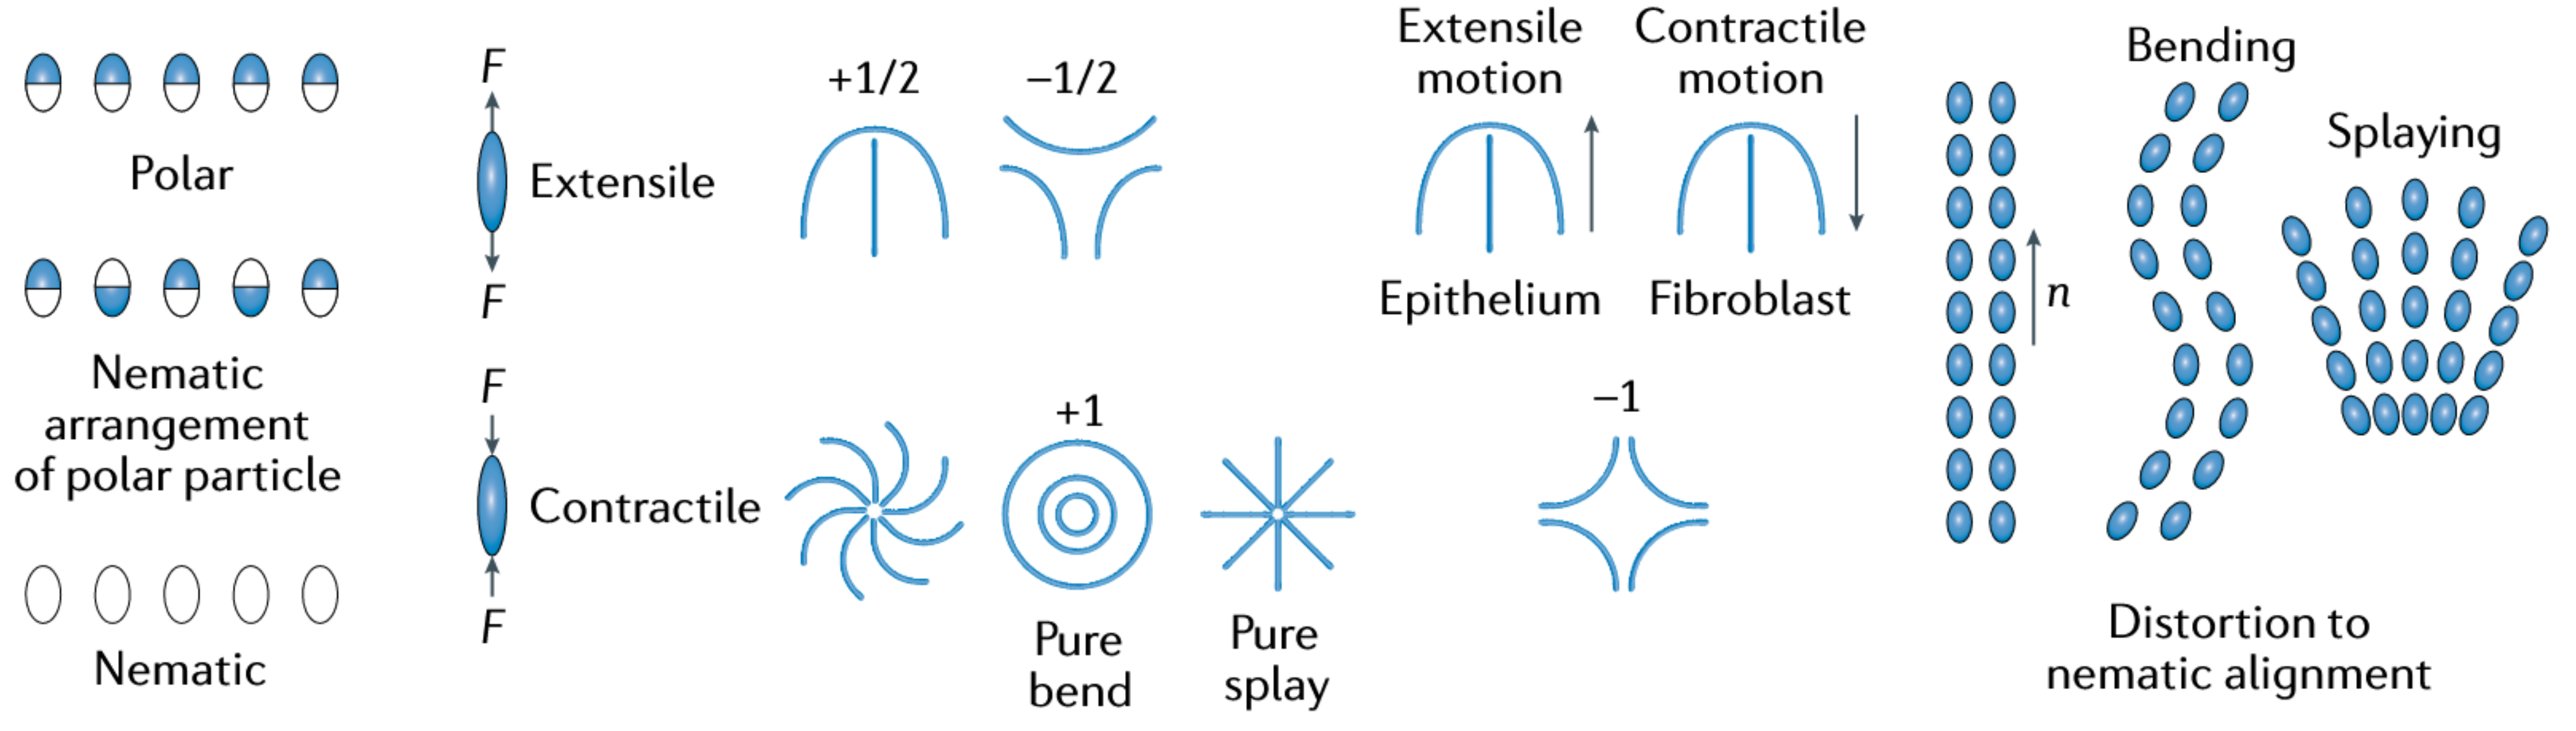
\includegraphics[width=\textwidth]{chap3nematic.png}
	\caption{\label{fig_3_10} \textbf{Active nematics}: Schematics of (A) nematic or polar particles, (B) extensile and contractile force dipoles, (C) Various types of defects and related motion of cells \textit{Adapted from \cite{xi2018}}. 
	}
\end{figure}

The utilization of this formulation is significant in characterizing the active forces produced by the network. The stress is separated into two components: active and passive. The passive stress arises from the viscoelasticity of the material and the bending, splaying, and twisting of the aligned elements. The active stress, on the other hand, is calculated by combining the strength of activity, represented by the parameter zeta, and the nematic order matrix. The sign of zeta determines the type of force dipole generated; a negative sign results in contraction of the system, while a positive sign leads to expansion along the nematic axis.

The active stress plays a crucial role in the motion of the system and can result in chaotic motion even in low Reynolds number systems, as evidenced in dense bacterial systems of \textit{Bacillus subtilis} where jet flows and turbulent patterns have been observed, as well as in expanding monolayers where independent vortices have been recorded \cite{wensink2012, blanch-mercader2018}. The nematic formulation have proven to be effective in capturing the physics of 2D confined systems and expanding systems (reviewed in \cite{saw2018}).

In the context of 3D models, active surfaces are used to describe the actomyosin cortex near cell membranes or epithelium in embryos \cite{salbreux2017}. This thin sheet of matter generates internal forces and torques that drive shape changes at the cellular or tissue level. The resulting three-dimensional structures can be conceptualized as curved, active two-dimensional surfaces. Forces and torques can be defined in terms of tension (\(t\)) and moment (\(m\)), and the model also considers the mirror and rotation symmetries of the surface elements (see fig \ref{fig_3_9}).
%
%\begin{figure}
%	\caption{\textbf{Active surface models}: (A) Tissues or cell surfaces can be modeled as surface with stresses and torques along the thickness. (B) Internal and external forces actin on a surface element. The kinematics of these surfaces, mathematical tools from differential geometry can be applied, using generalized coordinates ($\mathbf{X}$), metric tensor ($\mathbf{g}$), and curvature tensor ($\mathbf{C}$), where ($dl$) is the length of the line element with tangential unit vector ($v$). \textit{Adapted from \cite{salbreux2017}}}\label{fig_3_9}
%	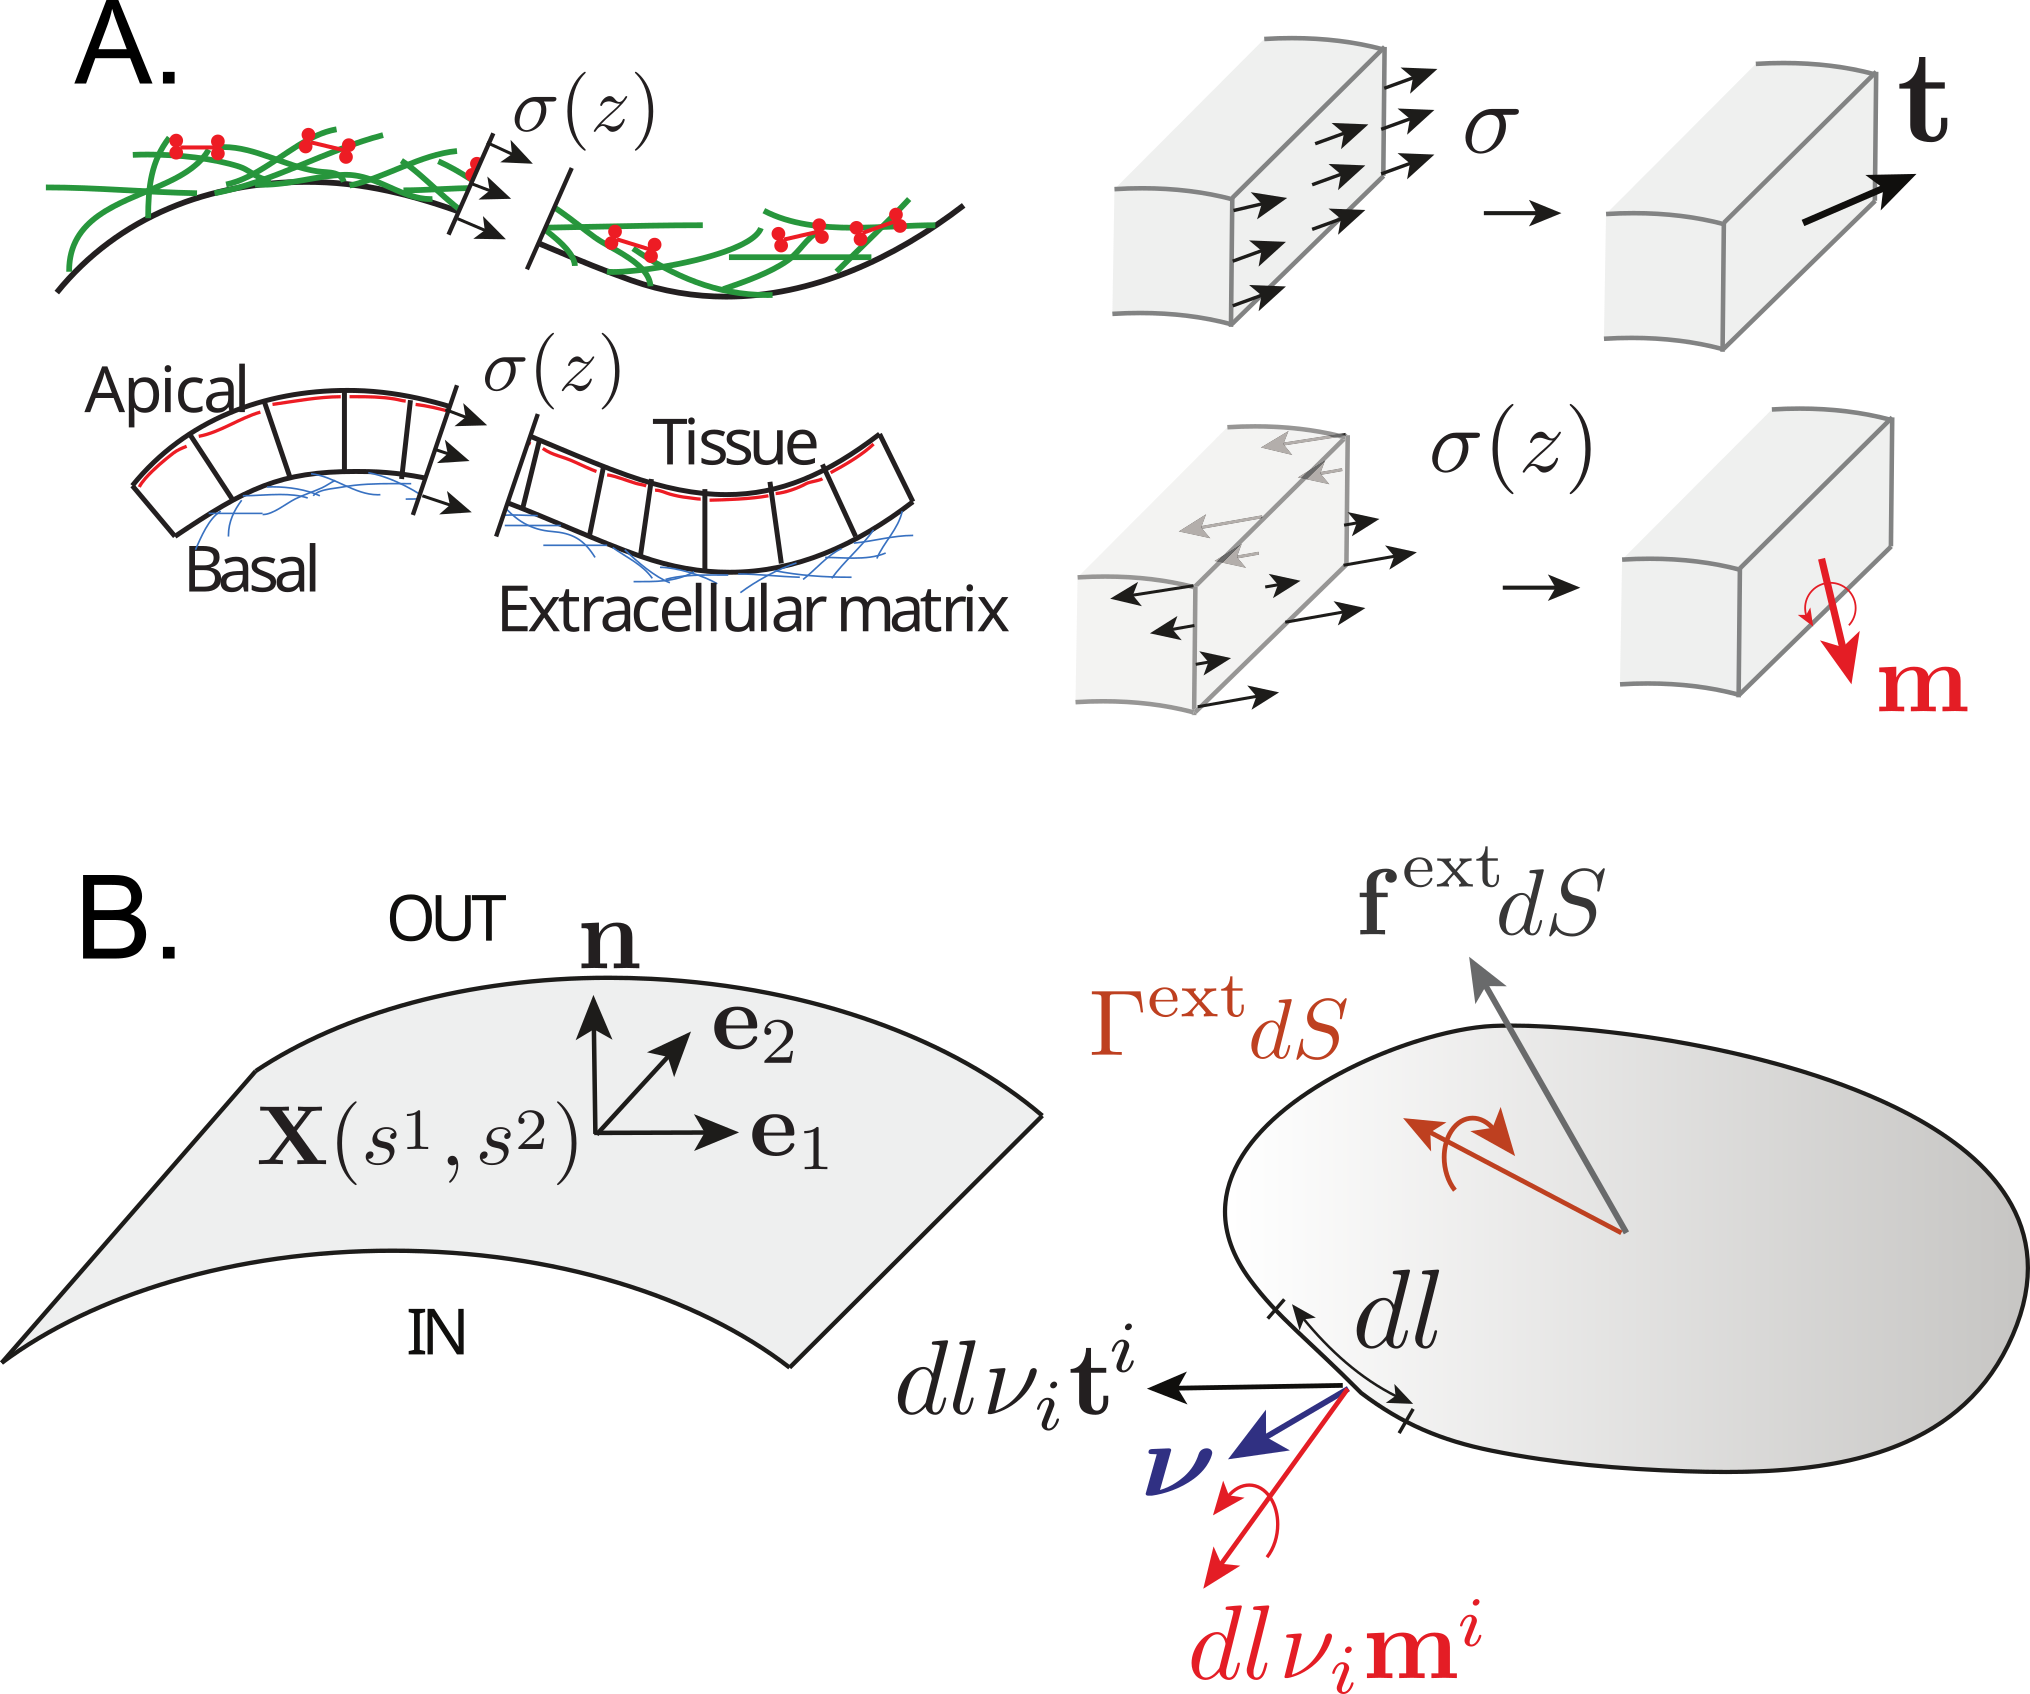
\includegraphics[width=7cm]{chap3activesurface.png}
%\end{figure} 
%

\begin{figure}
	\begin{minipage}[c]{0.5\textwidth}
		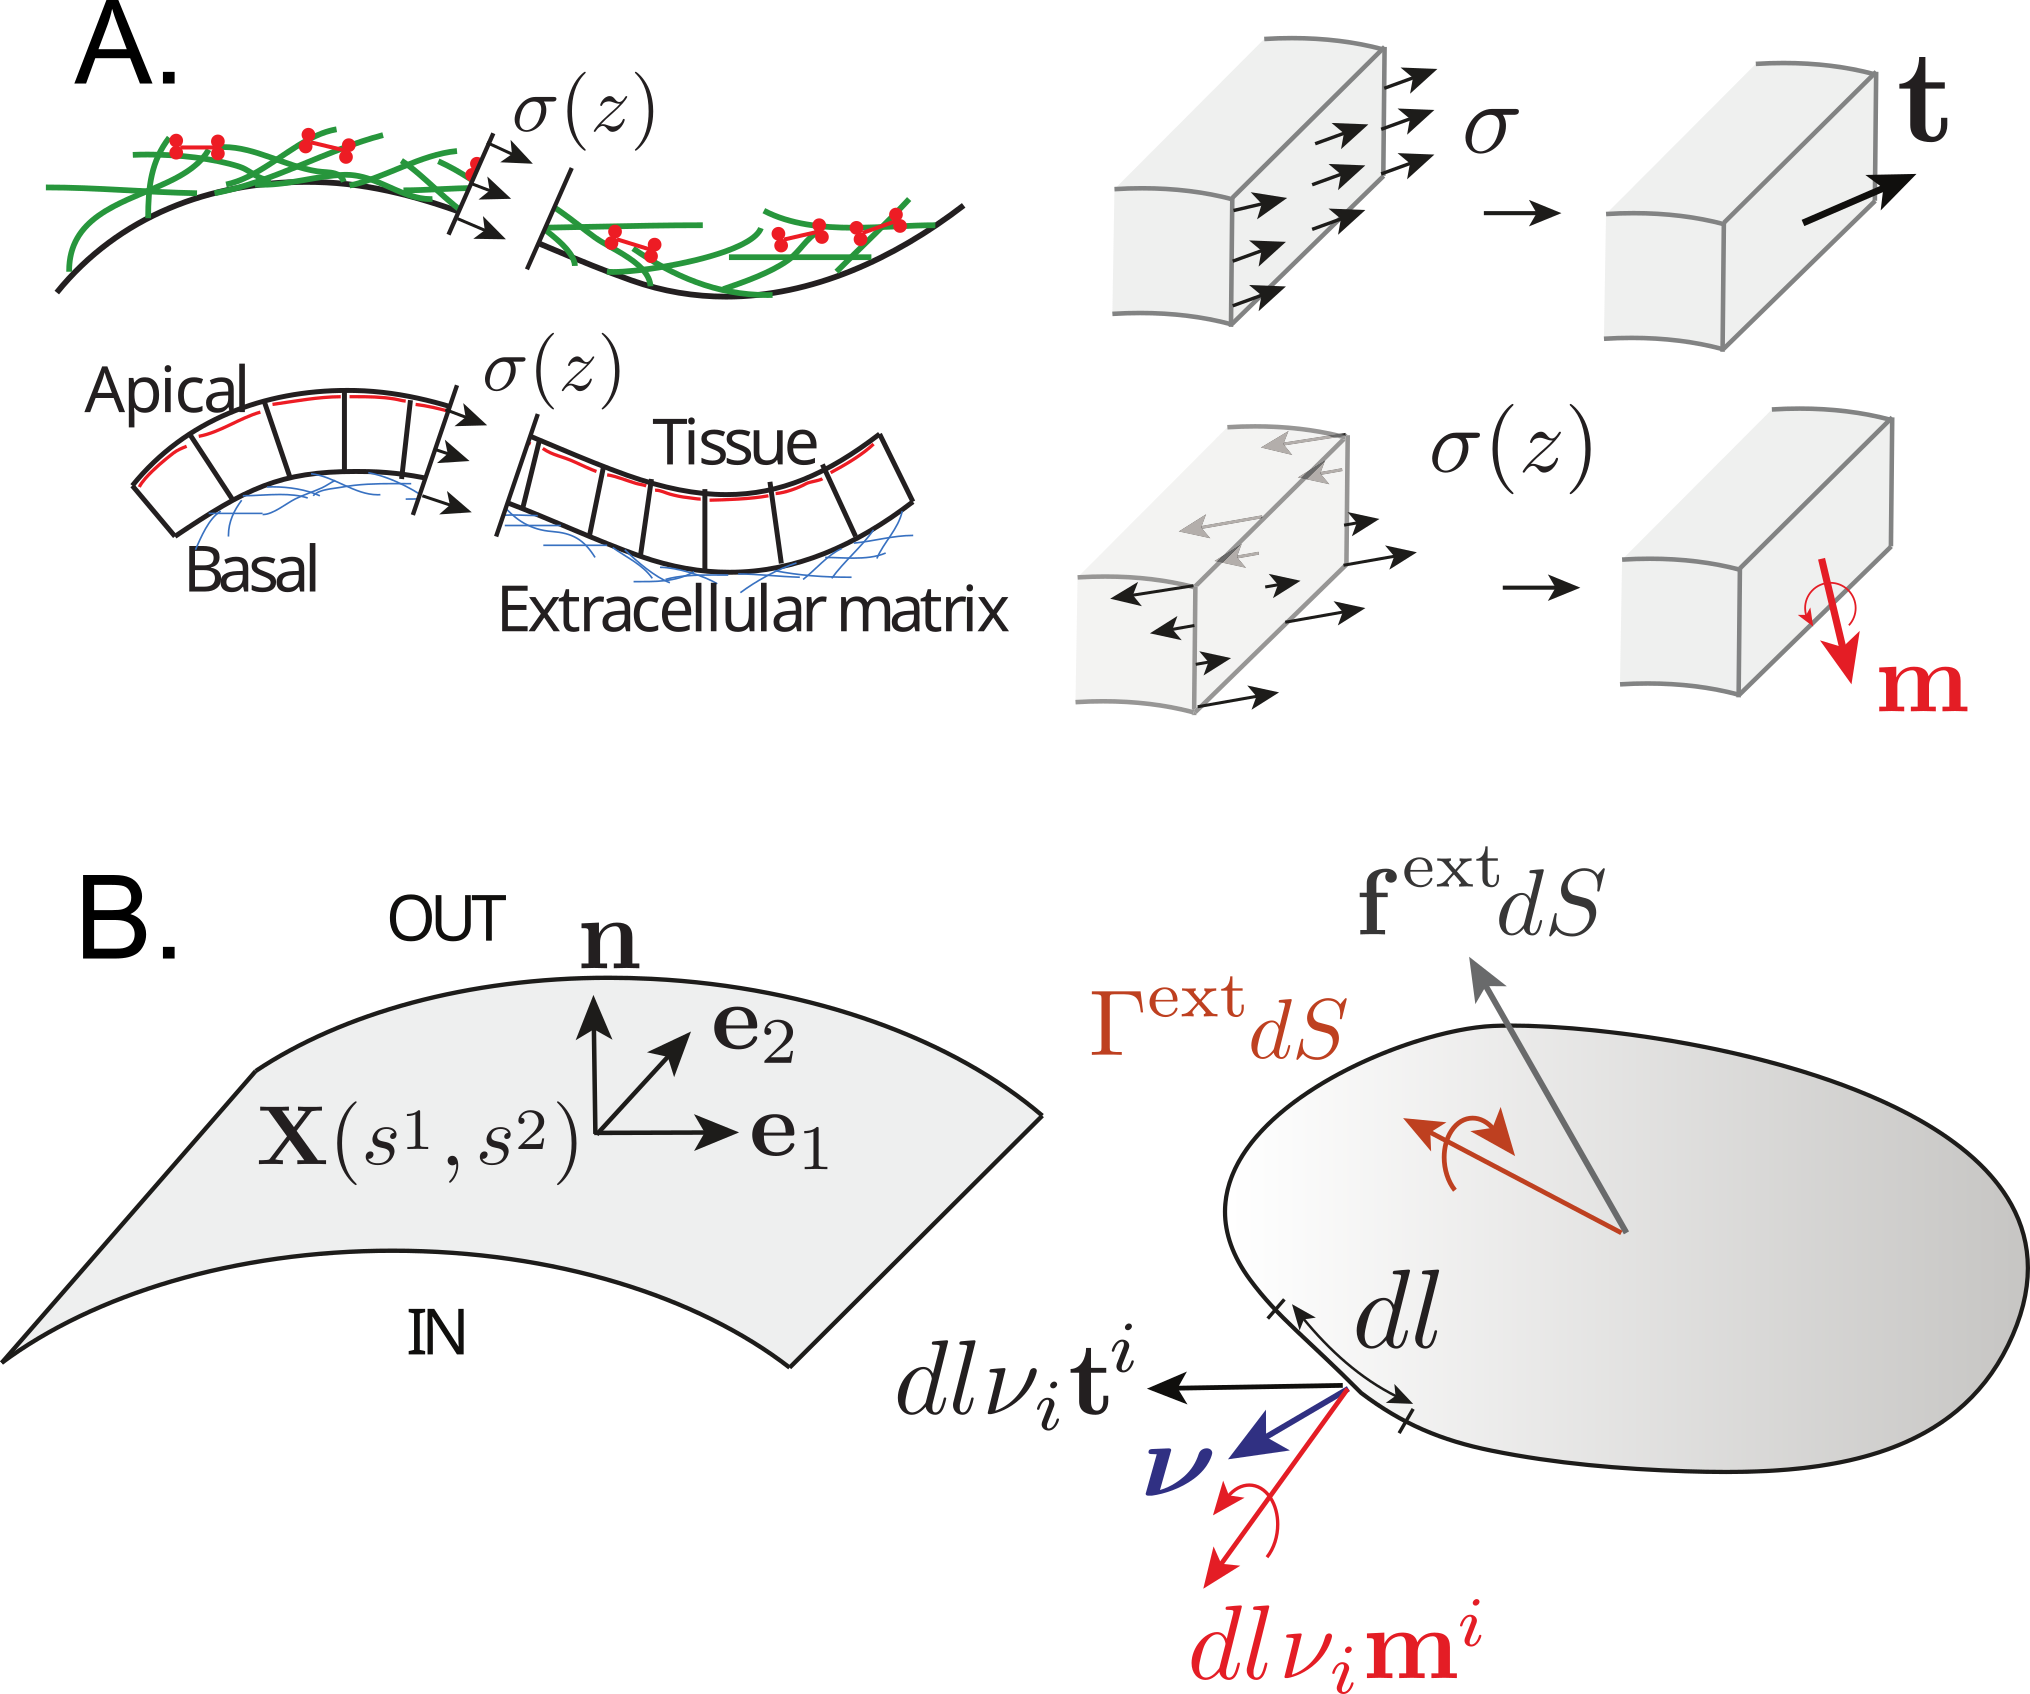
\includegraphics[width=\textwidth]{chap3activesurface.png}
	\end{minipage}\hfill
	\begin{minipage}[c]{0.45\textwidth}
		\caption{\textbf{Active surface models}: (A) Tissues or cell surfaces can be modeled as surface with stresses and torques along the thickness. (B) Internal and external forces actin on a surface element. The kinematics of these surfaces, mathematical tools from differential geometry can be applied, using generalized coordinates ($\mathbf{X}$), metric tensor ($\mathbf{g}$), and curvature tensor ($\mathbf{C}$), where ($dl$) is the length of the line element with tangential unit vector ($v$). \textit{Adapted from \cite{salbreux2017}}
		} \label{fig_3_9}
	\end{minipage}
\end{figure}





Salbreux and Julicher's work has demonstrated that flat active membranes with up-down asymmetry exhibit stability dependent on active tension and active tension-curvature coupling term. This tension-curvature dependency has been observed in the pancreas of mice, where the morphology of epithelial tumors is determined by the interplay of cytoskeletal changes in transformed cells and the existing tubular geometry \cite{messal2019}. Specifically, small pancreatic ducts produced exophytic growth, whereas large ducts deformed endophytically, consistent with theoretical predictions. Another example shows that curls of high curvature form spontaneously at the free edge of suspended epithelial monolayers, which originate from an enrichment of myosin in the basal domain that generates an active spontaneous curvature \cite{fouchard2020}. The extent of curling is controlled by the interplay between internal stresses in the monolayer.

While the molecular level behind epithelial morphogenesis, specifically the actin cytoskeleton, is well understood, there are still gaps in the theoretical and experimental framework that can bridge the gap between molecular dynamics and tissue-scale deformations. Vertex and continuum models have been developed to capture the physics of morphogenesis at the tissue scale, and phenomenological experiments provide insights into the constitutive relations of cytoskeletal components and tissues in specific conditions. However, combining vertex models and active surface mechanics could provide finer control over individual cell surfaces, enabling more precise bottom-up morphogenesis.

	\renewcommand{\thesection}{4.\arabic{section}}
	\hypertarget{bottom-up-morphogenesis}{%
	\chapter{Bottom up morphogenesis}\label{bottom-up-morphogenesis}}
	
\hypertarget{learn-by-building}{%
	\section{Learn by building}\label{learn-by-building}}

The mechanics and biology of epithelial tissues are complex, with mechano-chemical signaling and multiscale behavior all intertwined. The lens of active material has been instrumental in illuminating the role of molecular elements in undergoing shape changes during morphogenesis. Mechanistic understanding has been enhanced with new mathematical tools and advanced microscopy, enabling measurement of the forces involved in tissues.

The traditional and successful method for studying mechanics has been to deconstruct the system one component or parameter at a time. By manipulating genes or disrupting cellular processes, we can observe how mechanics change. This perturbative method allows for the alteration of biological systems at various levels, from molecular to tissue, (see fig \ref{fig_4_1}) .

However, studying systems like organoids or embryos can only provide limited physical insights into the topological transitions of these structures, as experimental systems have limited physical control and ability to measure forces. An alternative approach is to learn by actively performing morphogenesis or reconstructing biological structures from their basic components.

\begin{figure}
	\centering
	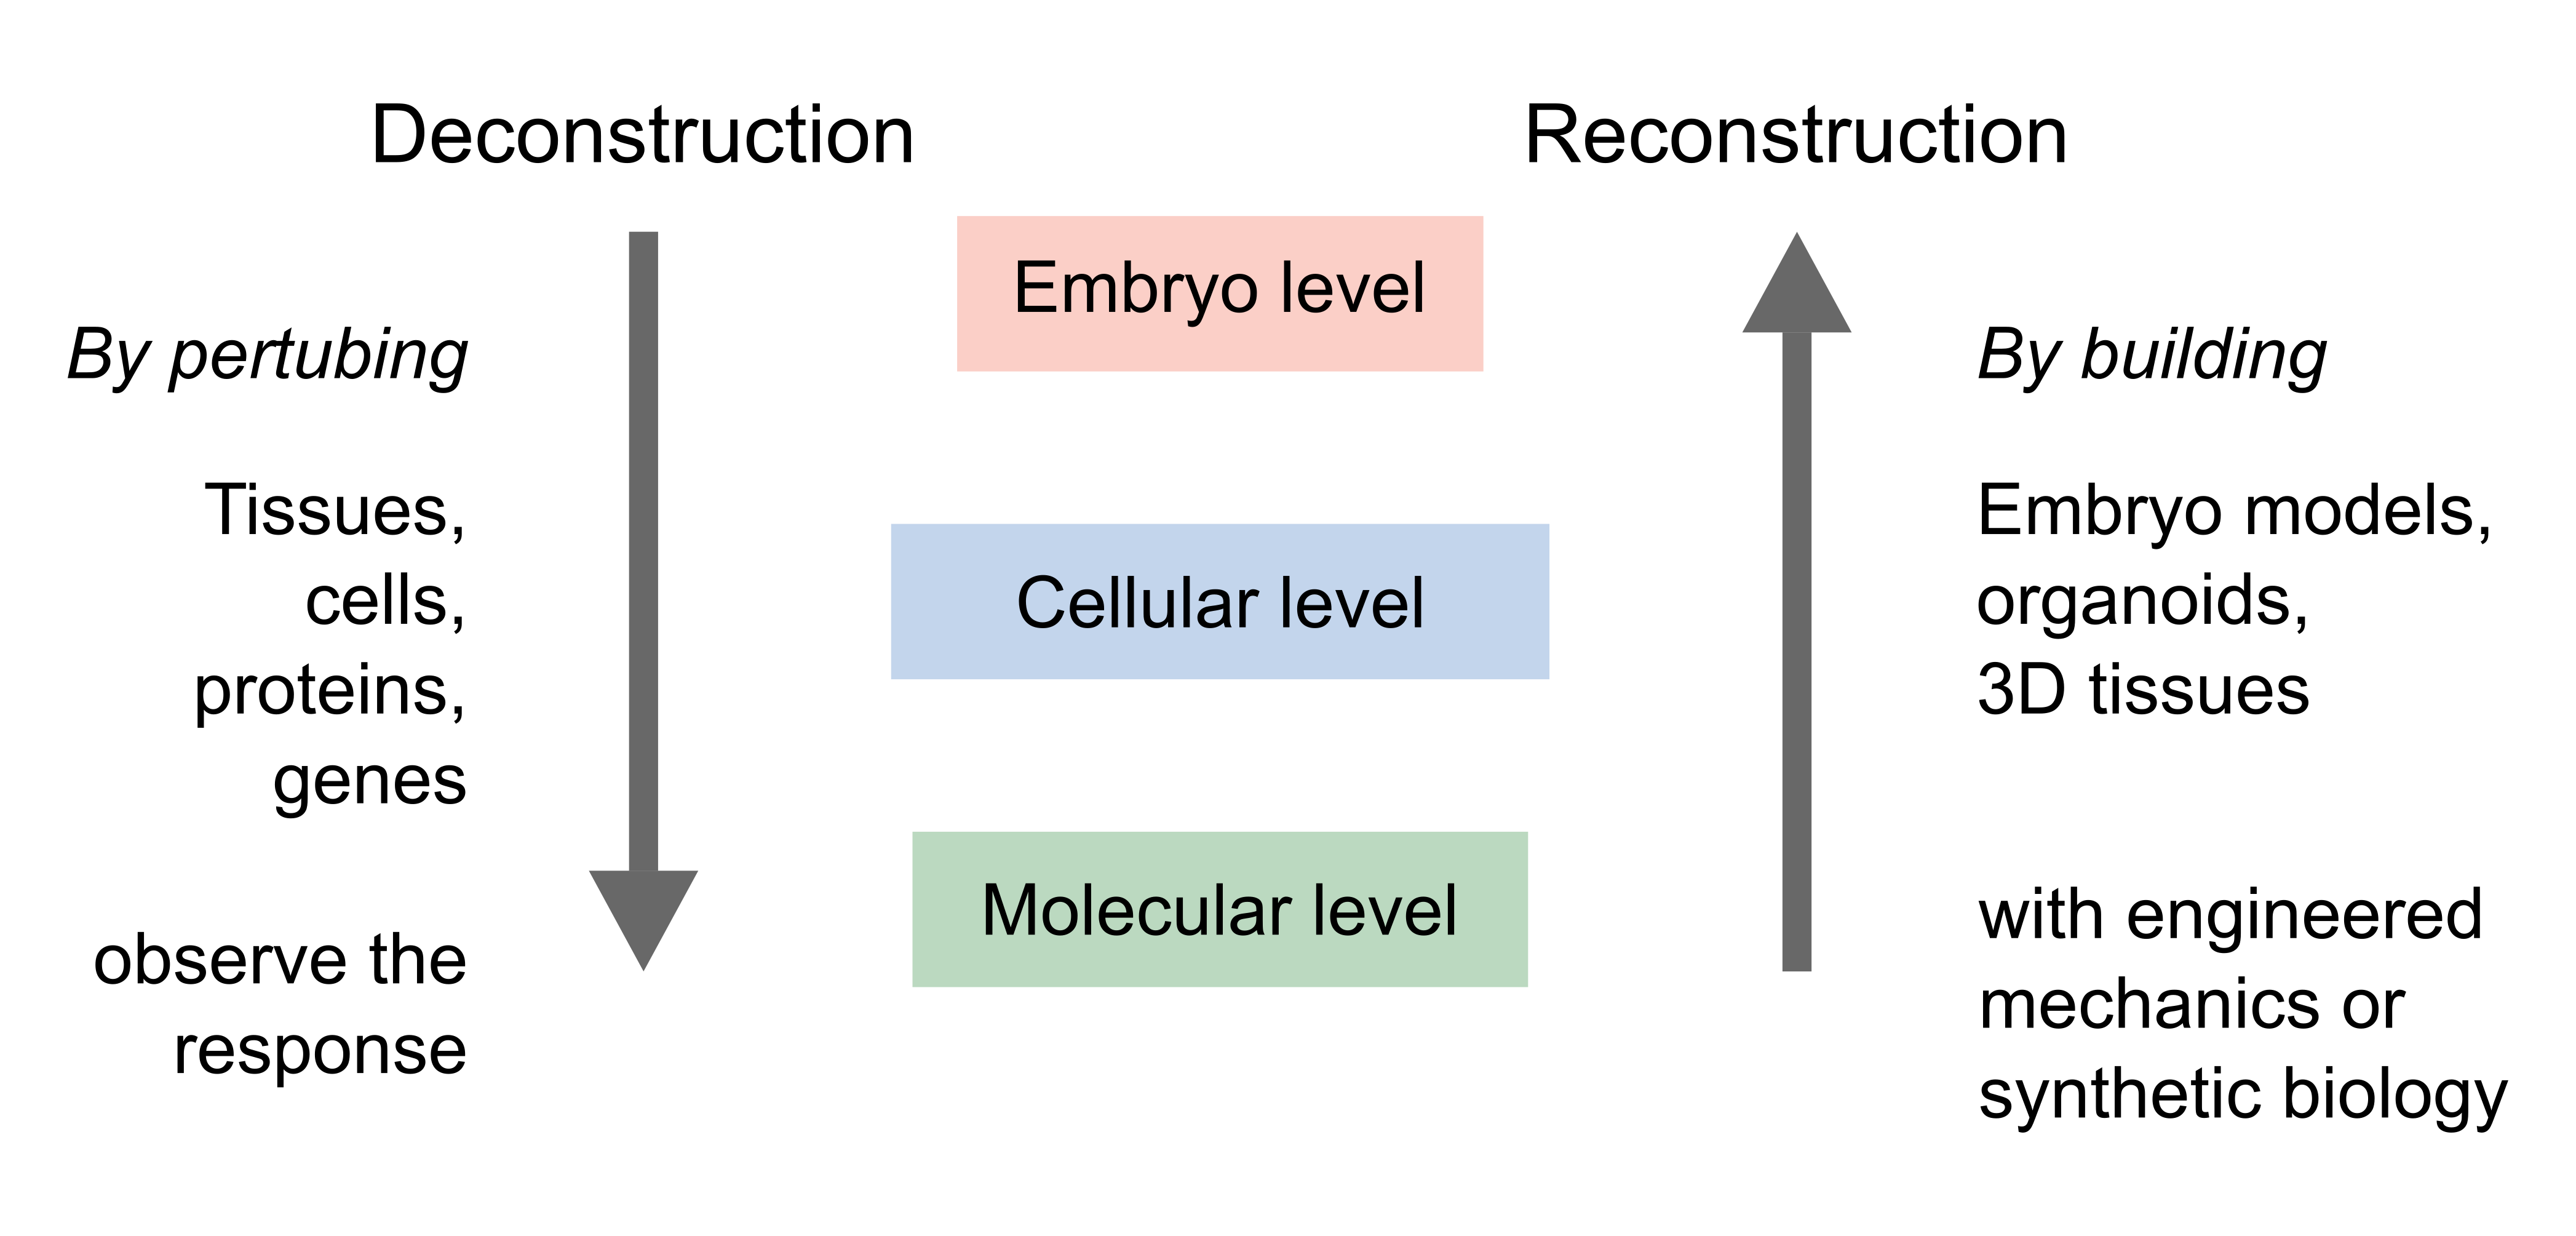
\includegraphics[width=0.65\textwidth]{chap4building.png}
	\caption{\label{fig_4_1} \textbf{A conceptual representation of two approaches to understanding mechanics: reconstruction (bottom-up) and deconstruction (top-down).} In reality, they are not separate from each other. These methods inform each other, with past top-down research guiding new reconstruction, and new engineered cells or tissues furthering our understanding of the field in innovative directions.
}
\end{figure}

For years, researchers have broken down biological systems into approachable parts - tissues, cells, proteins - in order to understand the behavior of each component. However, combining existing knowledge of these parts to recreate novel experimental systems could reveal the basic building blocks and effects of scale. This approach would complement top-down approaches in developmental biology. Synthetic biology, a perfect example of reconstruction, seeks to recreate life at various scales, from synthetic proteins to entire cells, in order to gain a deeper understanding of the indispensable components of life.

As active agents exist at every scale, emergent properties can appear at higher scales. Thus, it is essential to focus on higher scales or work with collectives of cells. This reminds me of the example of cars and traffic: Imagine you know the behavior of all individual car components, but this information is not sufficient to understand the behavior of traffic flow. This requires a higher level of analysis. 
\footnote{Matthew Good's commentary provides an insightful perspective on the complexity involved in building cells from interacting molecules. Meanwhile, Xavier Trepat argues that a bottom-up approach does not fully explain the emergent behavior of higher-level structures and emphasizes the need for constructing tissues at the mesoscale. Trepat uses the analogy of traffic jams to illustrate the importance of considering the collective behavior of cells in tissue engineering \cite{good2018}.} 
Similarly, biological structures exhibit numerous collective behaviors, such as jamming, nematic order, instabilities, or self-organization \cite{trepat2018}. 

Recreating structures from scratch also provides an opportunity to understand the role of physics at different scales. In the spirit of D'Arcy Thompson, we can explore the fundamental properties of matter in biological structures.
\footnote{. Thompson writes,’...to seek not for ends but for antecedents is the way of the physicists, who finds causes in what he has learned to recognize as fundamental properties, or inseparable concomitants, or unchanging laws, of matter and of energy.” \cite{thompson1979}}
For instance, we can study the role of surface tension in guiding the shape of cellular aggregates or lumens. In this work, we focus on the mesoscale structures of epithelia \((\sim 10-10^4 \mu m)\).  

We present our efforts to engineer an epithelial structure with a controlled microenvironment that is sensitive to self-organization and mechanical instabilities. The following sections will describe the ways of creating these structures from minimal ingredients.

\hypertarget{how-to-build-tissue-structures}{%
	\section{How to build tissue 		structures?}\label{how-to-build-tissue-structures}}

Before embarking on the construction of a tissue structure, it is important to consider the desired form and function. Despite the diversity in the shapes and functions of tissues, certain elementary shapes can be seen in many cases, resulting from the interplay between physical forces and biochemical signaling. Examples of such shapes include spherical blastocysts, ellipsoidal embryos, or cylindrical vessels.

After considering the desired form and function of the structure, established cell lines are selected and synthetic structures are constructed using various techniques, such as geometry control and localized folding, as discussed in the \ref{mechanobiology} section. The resulting structures can be further studied to understand the interplay between physical forces and biochemical signaling, as well as their potential applications in various biological systems.

\hypertarget{controlling-geometry-and-physical-forces}{%
	\subsection{Controlling geometry and physical 		forces}\label{controlling-geometry-and-physical-forces}}

From an engineering perspective, scaffolding is a commonly used approach for constructing synthetic epithelial structures. Scaffolds can be generated through 3D printing or microfabrication techniques, and cells can then be seeded onto the scaffold to attain the desired shape \cite{torras2018}. This method allows for the creation of a well-controlled microenvironment for the cells in terms of geometry, stiffness, adhesion proteins, and cell culture media (see fig \ref{fig_4_2} A) . Structures generated through this approach can be utilized to investigate tissue behavior in response to forces and curvature.

For instance, cells can be used to form a micro-vessel using a hydrogel with a cylindrical hole \cite{dessalles2021}. The hydrogel and cells were housed in a microfluidic device that controlled pressure and flow in the vessel, and the authors were able to examine the role of hydrogel poroelastic properties in regulating the dynamics of the vessel. Another exciting study demonstrated the potential of epithelial tissues to form shape-programmable materials by using a collagen scaffold \cite{mailand2022}.

Scaffolds can also be designed to dynamically change their shape (see fig \ref{fig_4_2} B). For example, a cell monolayer on a flexible membrane can alter its curvature \cite{blonski2021}, and a combination of stretching and unstretching a cell-laden hydrogel can produce distinctive folds and patterns \cite{chan2018}. In some cutting-edge studies, researchers have utilized 4D bioprinting, where 3D printed objects undergo transformation over time \cite{arif2022}. For instance, a flat hydrogel sheet containing endothelial cells and photo-crosslinking can be transformed into a tube \cite{zhang2020}.


\begin{figure}
\centering
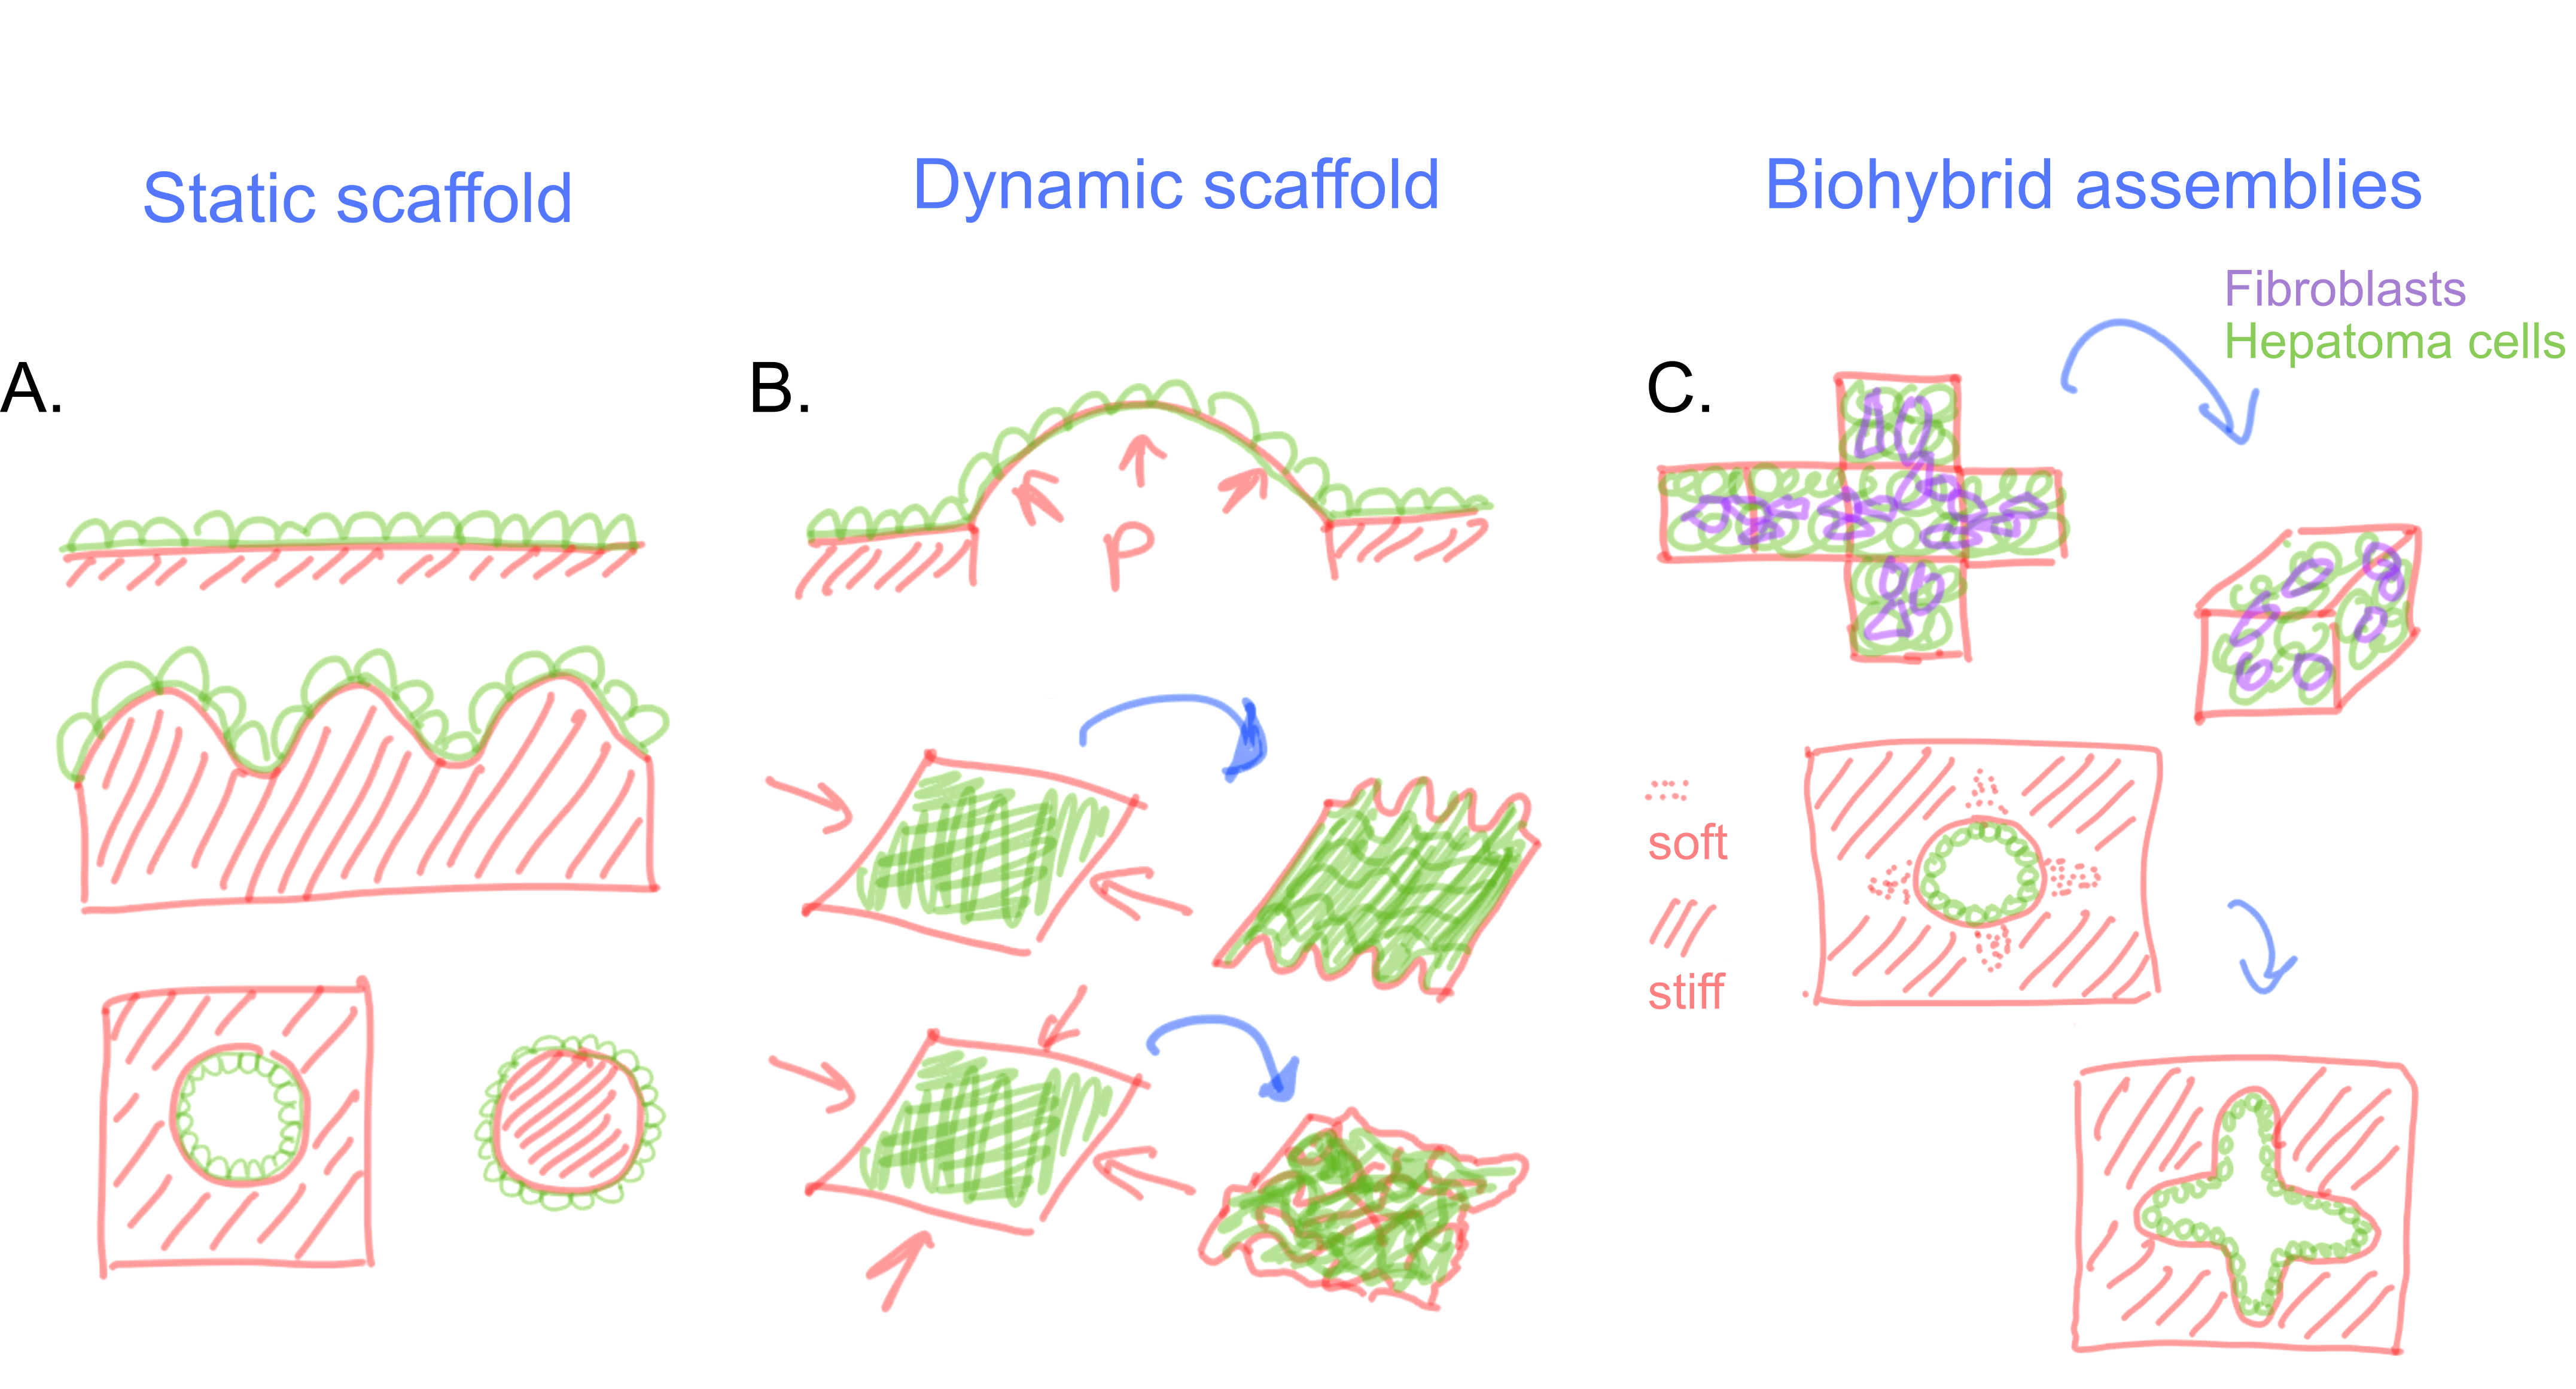
\includegraphics[width=\textwidth]{chap4scaffold.png}
\caption{\label{fig_4_2}\textbf{Controlling geometry and physical forces: } The concept of scaffolding can be divided into two categories: static and dynamic scaffolds. (A) Static scaffolds are microfabricated structures that cells can adapt to and respond to geometrical cues, leading to the formation of a specific tissue organization \cite{brassard2021}. (B) In contrast, dynamic scaffolds consist of cell-laden matrices that are deformable, and their curvature can change dynamically due to external pressure or mechanical forces \cite{blonski2021, chan2018}. (C) Biohybrid assemblies can incorporate active contraction or pushing to create hybrid structures, such as origami folding triggered by fibroblast contraction \cite{he2018}, or cells carving out an intestinal crypt-like geometry from a softer matrix \cite{gjorevski2016}.}
\end{figure}

Additionally, the contractility of fibroblasts and hepatoma cells has been utilized to fold 2D structures into 3D shapes \cite{he2018} (see fig \ref{fig_4_2} C) . Microplates with an origami folding pattern are created, and the cells apply forces to generate a 3D structure. In other scenarios, cells are allowed to self-organize through the imposition of geometric constraints, which enhances the efficiency of organoid-like systems \cite{gjorevski2016}. In the case of intestinal organoids, controlling the stiffness of the matrix in specific regions leads to growth and differentiation at softer areas, producing a highly reproducible structure \cite{gjorevski2022}.

\hypertarget{manipulating-biochemical-signaling}{%
	\subsection{Manipulating biochemical signaling}\label{manipulating-biochemical-signaling}}

Another approach to constructing biological structures involves controlling biochemical signaling to induce shape transformation. This approach utilizes natural processes in embryo morphogenesis, such as apical constriction in ventral furrow formation or cell jamming in the normal elongation of the zebrafish. Optogenetic tools, such as controlling Rho signaling, can be used to induce localized apical constriction with spatiotemporal control \cite{izquierdo2018}. This technique can also be applied to other proteins, such as Shroom3, to induce synthetic morphogenesis in neural organoids \cite{martinez-ara2022} (see fig \ref{fig_4_3} C).

Epithelial-mesenchymal interaction is another crucial aspect of the tissue folding process. Hughes et al. demonstrated that cell clusters can remodel the matrix to create oriented stresses that lead to budding in tissues \cite{hughes2018}. By controlling the location and density of these cell clusters, it is possible to manipulate the curvature of the epithelia. Mesenchymal condensation serves as a folding template for the final tissue structure \cite{palmquist2022, shyer2017} (see fig \ref{fig_4_3} B).

The microenvironment plays a critical role in providing vital signals to tissues and can be manipulated to activate specific cellular functions. Microfluidic techniques can deliver appropriate morphogen gradients to the tissue with precise timing \cite{hofer2021}. \textit{In vivo}, multiple morphogens often act simultaneously. For instance, during neural tube development, there is an opposing gradient of sonic hedgehog (SHH) and bone morphogenic protein (BMP). With microfluidic devices, stable gradients can be generated, even in opposite directions \cite{demers2016}, thus mimicking symmetry-breaking events and directional neural tube patterning (see fig \ref{fig_4_3} D).

Moreover, genetic engineering of specific cells can be utilized to control signaling. Human pluripotent stem cells (hPSCs) can be programmed to express SHH \cite{cederquist2019} (see fig \ref{fig_4_3} E). Mixing these cells with others could result in a polarized organoid and a patterned cerebral organoid.

\begin{figure}
	\centering
	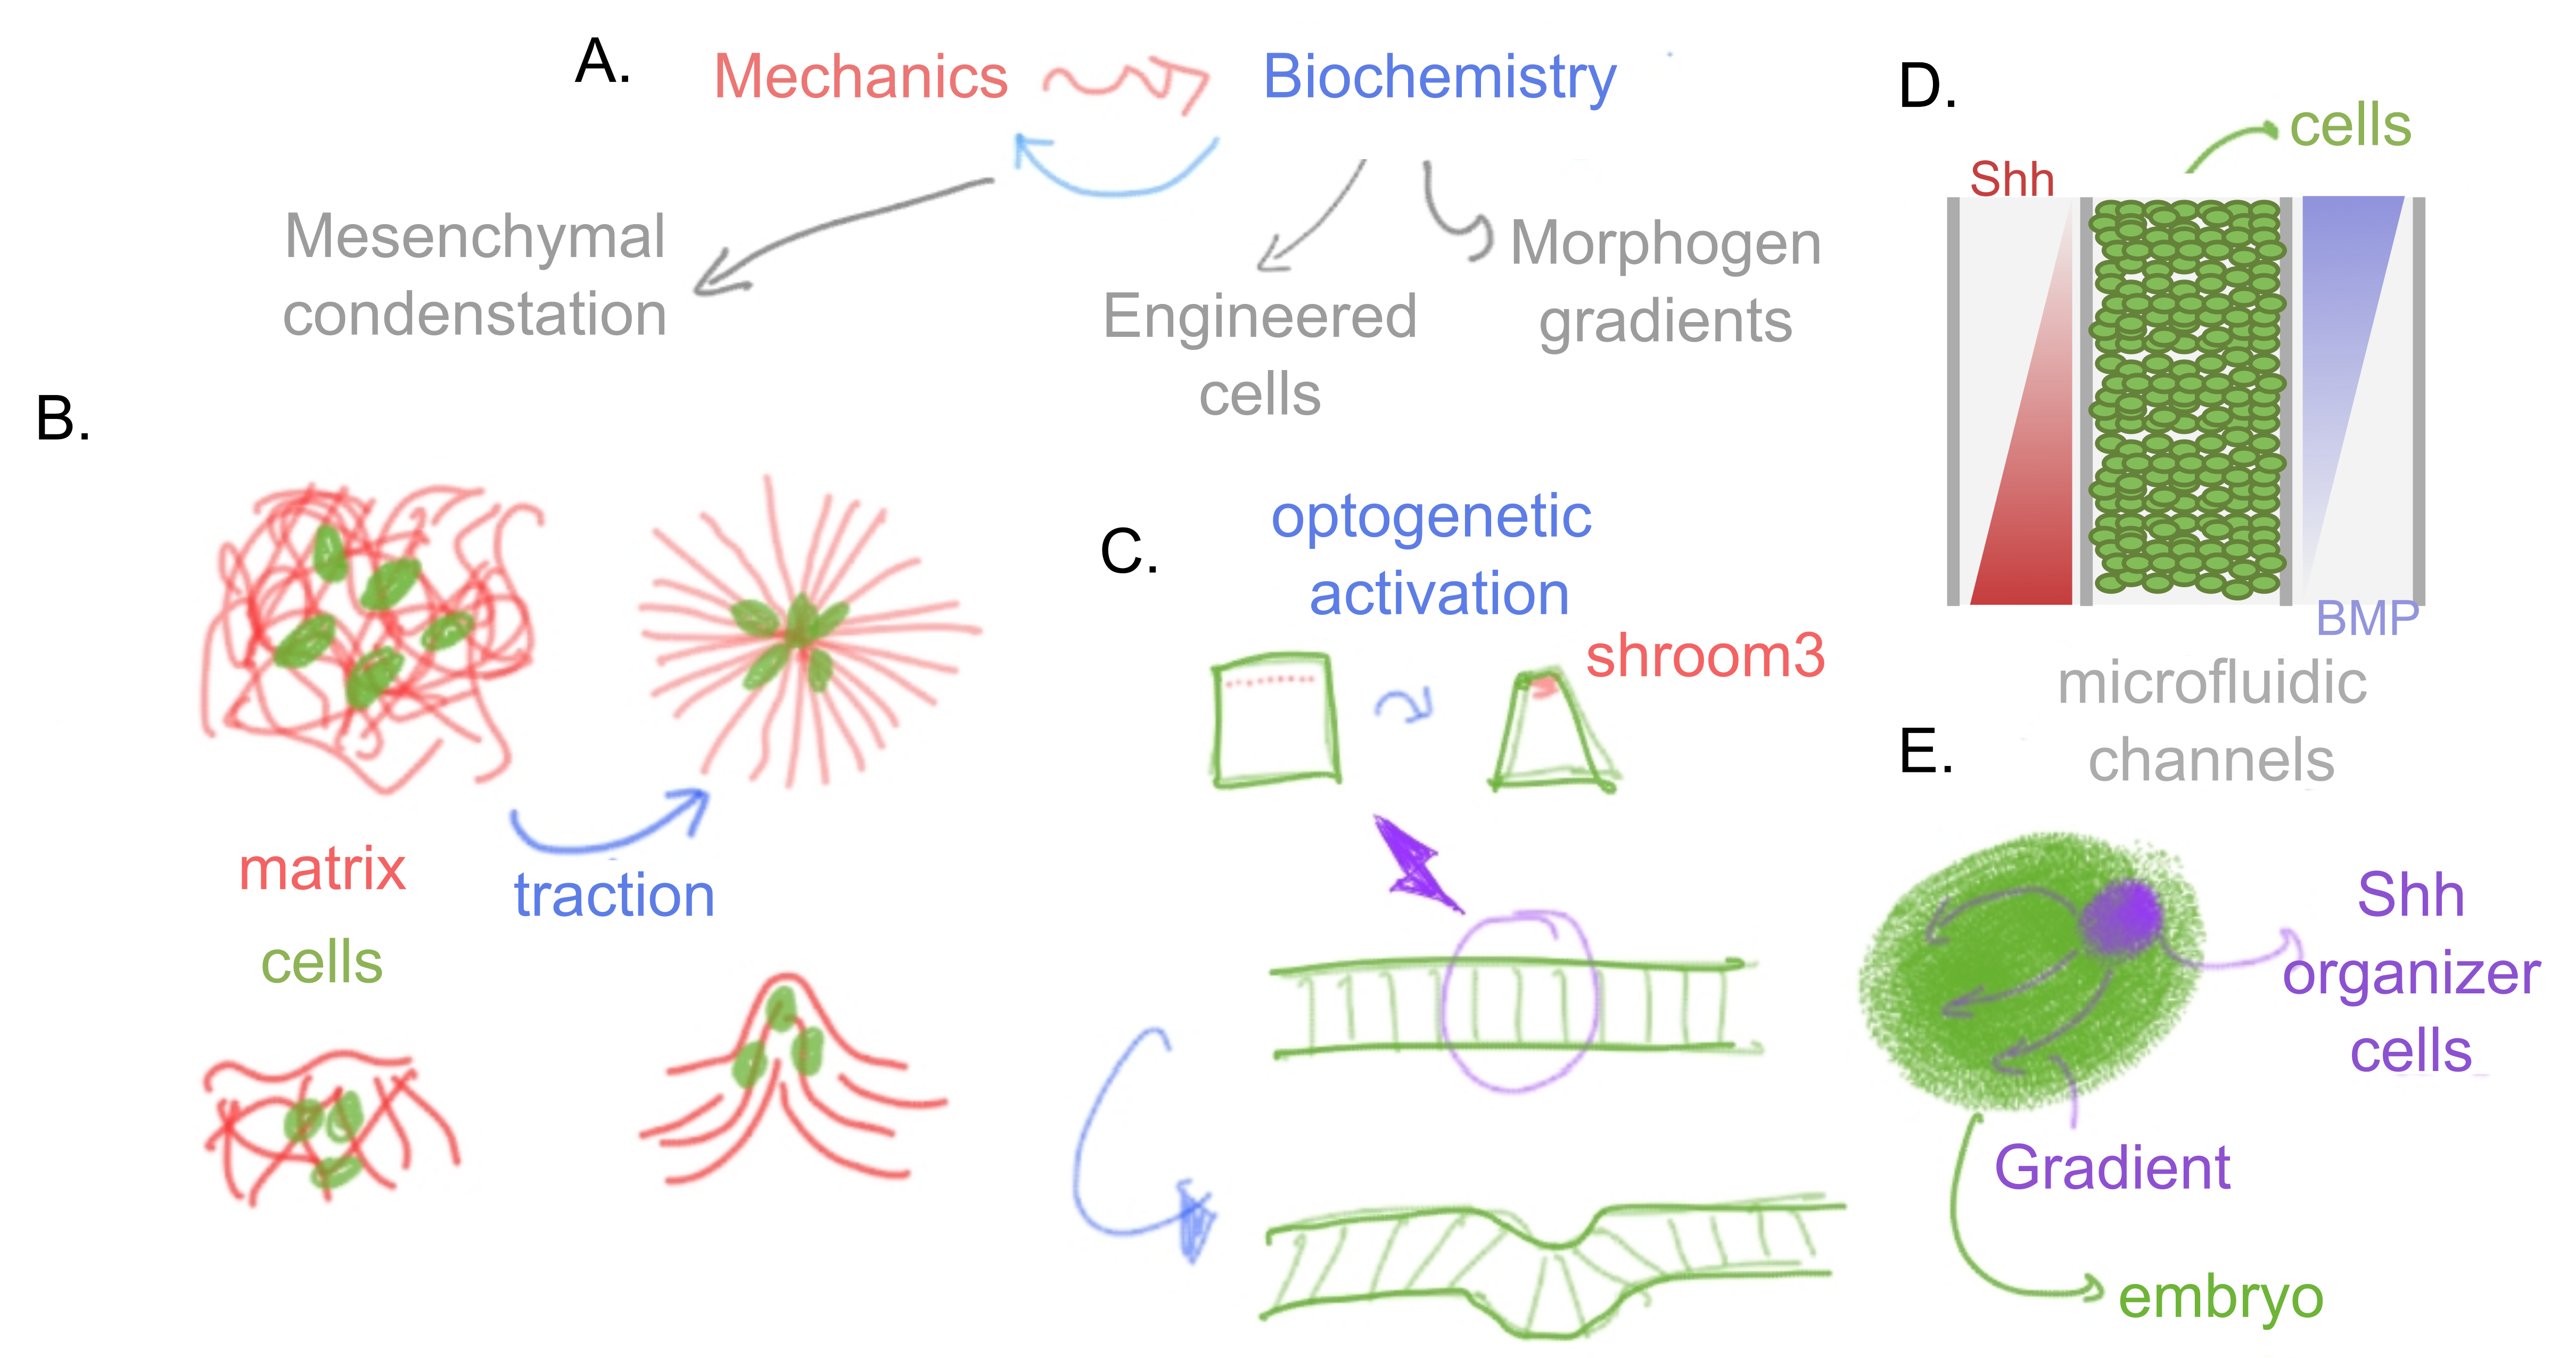
\includegraphics[width=\textwidth]{chap4biochem.png}
	\caption{\label{fig_4_3} \textbf{Manipulating biochemical signaling:} Biochemical signaling and mechanics are interdependent in morphogenetic processes (A). The transport of signaling molecules can affect the cytoskeleton and mechanical properties of cells, while mechanical forces can also influence biochemical signaling. Microfluidics (D) is one method used to control biochemical signaling by providing opposing morphogen gradients through multiple channels \cite{demers2016}. Alternatively, cells can be genetically engineered to undergo apical constriction (C) or produce morphogen gradients (E) locally to form curved geometries \cite{martinez-ara2022, cederquist2019}. Mesenchyme condensation (B) is another approach used to program curvature in developing tissues \cite{hughes2018, palmquist2022}.}
\end{figure}

\hypertarget{exploiting-mechanical-instabilities}{%
	\subsection{Exploiting mechanical
		instabilities}\label{exploiting-mechanical-instabilities}}

\begin{figure}
	\centering
	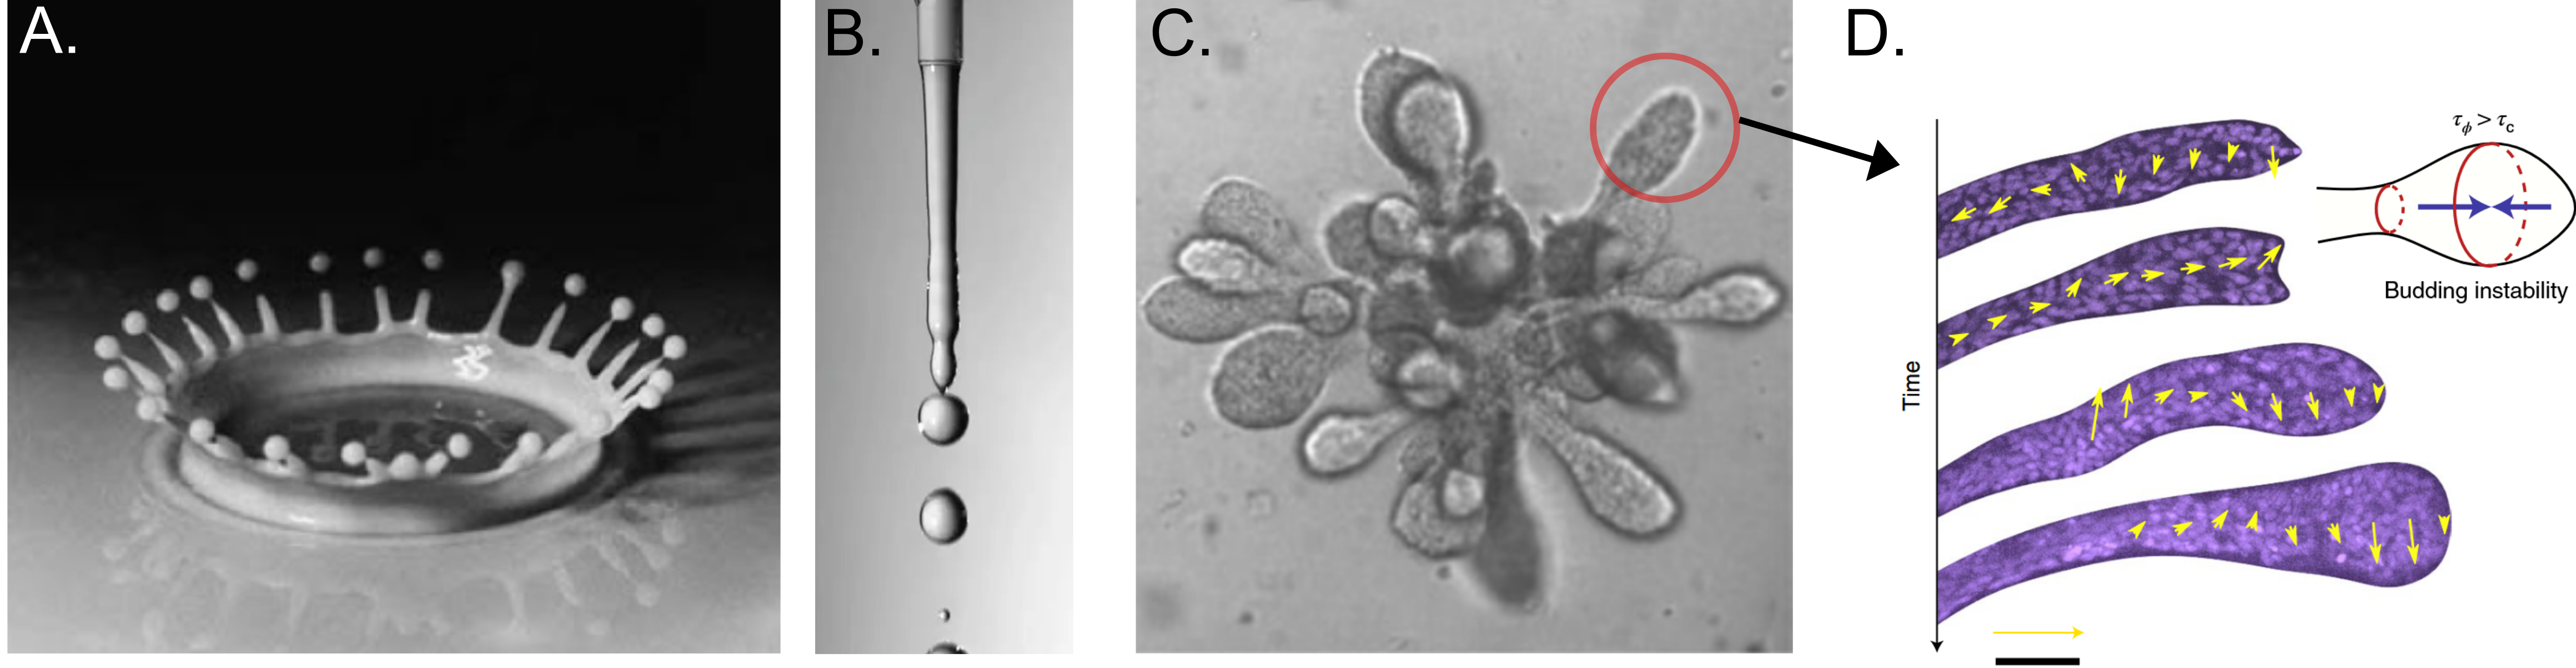
\includegraphics[width=\textwidth]{chap4rayleigh.png}
	\caption{\label{fig_4_4} \textbf{D'Arcy Thompson compares biological budding to splashes} (A) of fluids and Rayleigh-Plateau instability \cite{thompson1979} (B), where liquid splits up into smaller droplets. This mechanism could also be seen in organogenesis of mammary tissue (C, D) \cite{fernandez2021}.}
\end{figure}

Morphogenesis, the process of shaping and formation of biological structures, often involves spontaneous pattern formation or symmetry-breaking events \cite{ishihara2018}. These processes are often dictated by mechanical instabilities, which can lead to large deformations in soft matter systems. In material science, these instabilities are typically seen as problematic as they cause rapid breakage. However, in soft matter, large deformations can lead to interesting topological transformations, providing an opportunity for engineers to exploit these instabilities in the development of new actuators or soft robots (reviewed in \cite{pal2021}).
\footnote{"Mechanical instabilities have provided a unique approach to imbue “material intelligence” into soft machines without requiring the addition of rigid components. For example, binary actuators relying on mechanical instabilities can recreate logic modules and reproduce valving functionality using entirely soft elements.}

The significance of mechanical instabilities was foreseen by D'Arcy Thompson in his comparison of fluid splashes to hydroids (see fig \ref{fig_4_4} A). He wrote that the shapes of a potter's cup, glass blower's bulb, and biological structures are simply glorified splashes formed slowly under conditions of restraint that enhance or reveal their mathematical symmetry \cite{thompson1979}.
\footnote{ I cannot recommend enough the chapter “the forms of cell”. He states “Many forms are capable of realization under surface-tension, … The subject is a very general one; it is, in its essence, more mathematical than physical; it is part of the mathematics of surfaces, and only comes into relation with surface-tension because this physical phenomenon illustrates and exemplifies, in a concrete way, the simple and symmetrical conditions with which the mathematical theory is capable of dealing.”}
This conjecture has been confirmed through numerous quantitative studies on various systems, including ripples in leaves and wrinkles in the brain \cite{liang2009, karzbrun2018}.

There are various instabilities associated with solids and fluids. For example, the Rayleigh-Plateau instability explains why a fluid stream breaks into smaller packets, driven by the fluid's tendency to minimize its surface area due to surface tension. The same instability can arise when fluid is surrounded by an elastic medium, instead of air, provided the surface tensions can overcome the elastic stresses, leading to budding as observed in alveologenesis in human mammary tissue \cite{fernandez2021} (see fig \ref{fig_4_4} C-D). However, as tissues are active viscoelastic materials surrounded by viscoelastic medium, the timescales of these instabilities change, slowing down to hours instead of milliseconds in water droplets.

There are several types of mechanical instabilities associated with solids and fluids, including Rayleigh-Plateau instability, Kelvin-Helmholtz instability, Rayleigh-Taylor instability, viscous coiling and folding, and large-scale wrinkling and buckling \cite{gallaire2017, kourouklis2018}. In this study, we aim to harness these instabilities to recreate epithelial structures.

Applying compressive stresses is one of the easiest ways to induce mechanical instabilities in solids. These stresses can occur in biological systems as a result of differential growth, swelling, or morphogen gradients and can lead to various forms of instabilities, including wrinkling, creasing, and buckling. Buckling occurs when a thin sheet is subjected to in-plane compressive stress, and if the stress is above a critical value, the sheet undergoes out-of-plane deformation instead of in-plane shrinkage (see fig \ref{fig_4_5} B). In contrast, wrinkling and creasing occur in similar compressive stresses, but the thin sheet is typically supported by a compliant substrate.

\begin{figure}
	\centering
	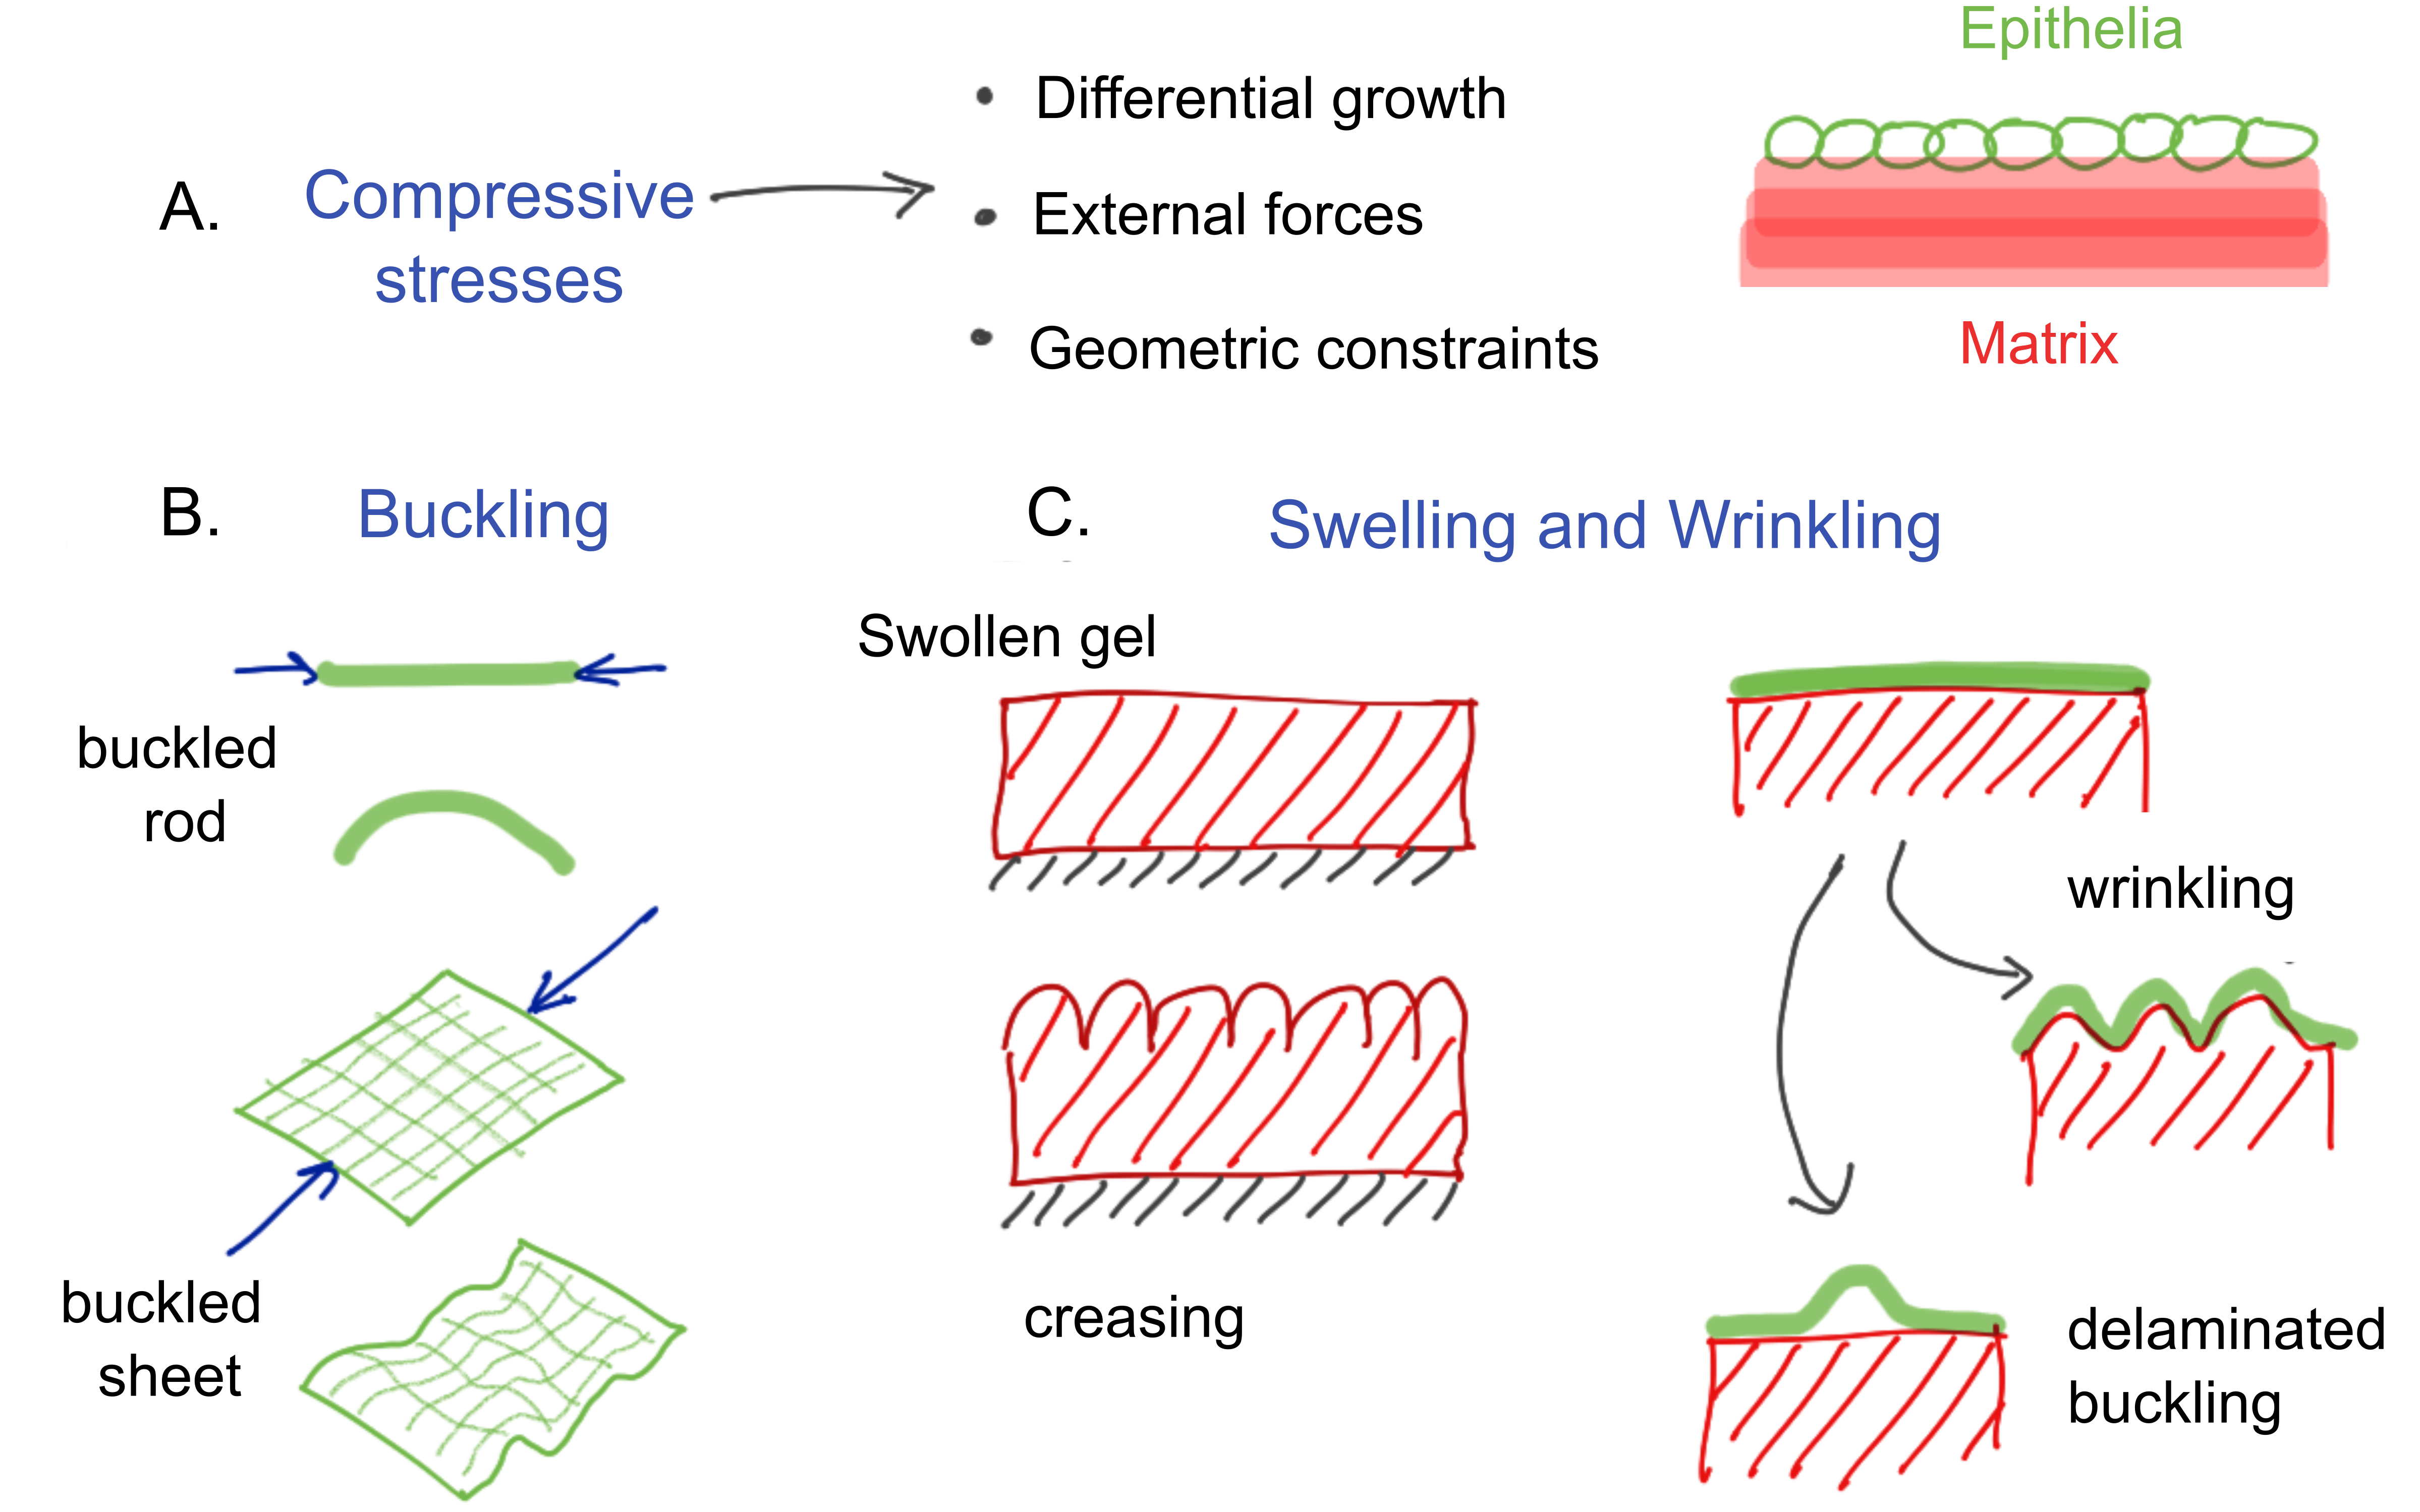
\includegraphics[width=0.8\textwidth]{chap4instabilites.png}
	\caption{\label{fig_4_5} \textbf{Compressive stresses} occur frequently in many systems (A). We can consider epithelia and matrix as thin sheet supported by a compliant substrate. Thus, the tissue folding could be understood as buckling of sheets (B) or wrinkling or creasing of thin film supported by an hydrogel (C).}
\end{figure}

The creation of biological tissues \textit{in vitro} has been a subject of great interest in the field of tissue engineering. To reproduce the characteristics of these tissues, researchers have turned to the use of hydrogels. These materials can be mechanically and chemically manipulated to simulate the behavior of biological matrices, which provide support for epithelial structures.

One of the ways in which hydrogels can be used to recreate the behavior of biological tissues is through the application of physical stress. For example, swelling of the hydrogel can cause it to undergo rapid large volumetric changes, producing crease-like patterns on the surface. If the hydrogel is constrained at the bottom, these creases can become permanent. Alternatively, if the hydrogel is supported by another flexible material, such as another hydrogel or an elastic substrate, the stresses produced during swelling will result in a wrinkling instability (see fig \ref{fig_4_5} A). These instabilities are important for understanding the formation of a variety of structures, including the gyrification of the brain cortex.

In a study by Tallinen et al., the gyrification of the brain cortex was replicated through the programming of materials to produce wrinkling \cite{tallinen2016}. The researchers created a synthetic brain with an inner core of an inert elastomer and an outer layer of a swellable elastomer. On swelling, the outer layer produced folds that closely matched the process of gyrification (see fig \ref{fig_4_6} A).

Similar mechanisms have been observed in other systems undergoing differential growth, such as the branching of lungs and formation of intestinal villi \cite{varner2015,shyer2013} (see fig \ref{fig_4_6} B,D). These findings highlight the potential of hydrogels as a tool for understanding the physical mechanisms underlying tissue development. However, it is worth noting that the mechanisms described here are the subject of ongoing research and debate in the field of developmental biology.

The ability to recreate biological tissue growth conditions \textit{in vitro} has been made possible through the use of hydrogels. Researchers have discovered that by mechanically and chemically controlling the hydrogel, they can generate desired mechanical instabilities \cite{dervaux2012}. This can be accomplished through the swelling or pre-stretching of the gel, or by manually applying compressive stresses.

One way to simulate growth is through the direct stretching or compression of the gel. Chan et al. showed that the patterns produced can be controlled by modulating the shear modulus of the hydrogel with the epithelial layer and stretch \cite{chan2018} (see fig \ref{fig_4_5} B). By pre-stretching the hydrogel before seeding cells, they were able to produce folded patterns with different wavelengths depending on the type of pre-stretching applied (uniaxial or biaxial). 

Another type of instability in bilayers is delaminated buckling, which is often observed in thin film delamination in furniture. This can be induced through compressive stresses created during growth or collective tension. Recent studies have shown that growing epithelia confined in a sphere undergo delaminated buckling after reaching a critical growth-induced stress \cite{trushko2020} (see fig \ref{fig_4_6} C), or through intercellular stresses \cite{oyama2021} or by placing a biofilm on top of the epithelial monolayer \cite{cont2020}.

\begin{figure}
	\centering
	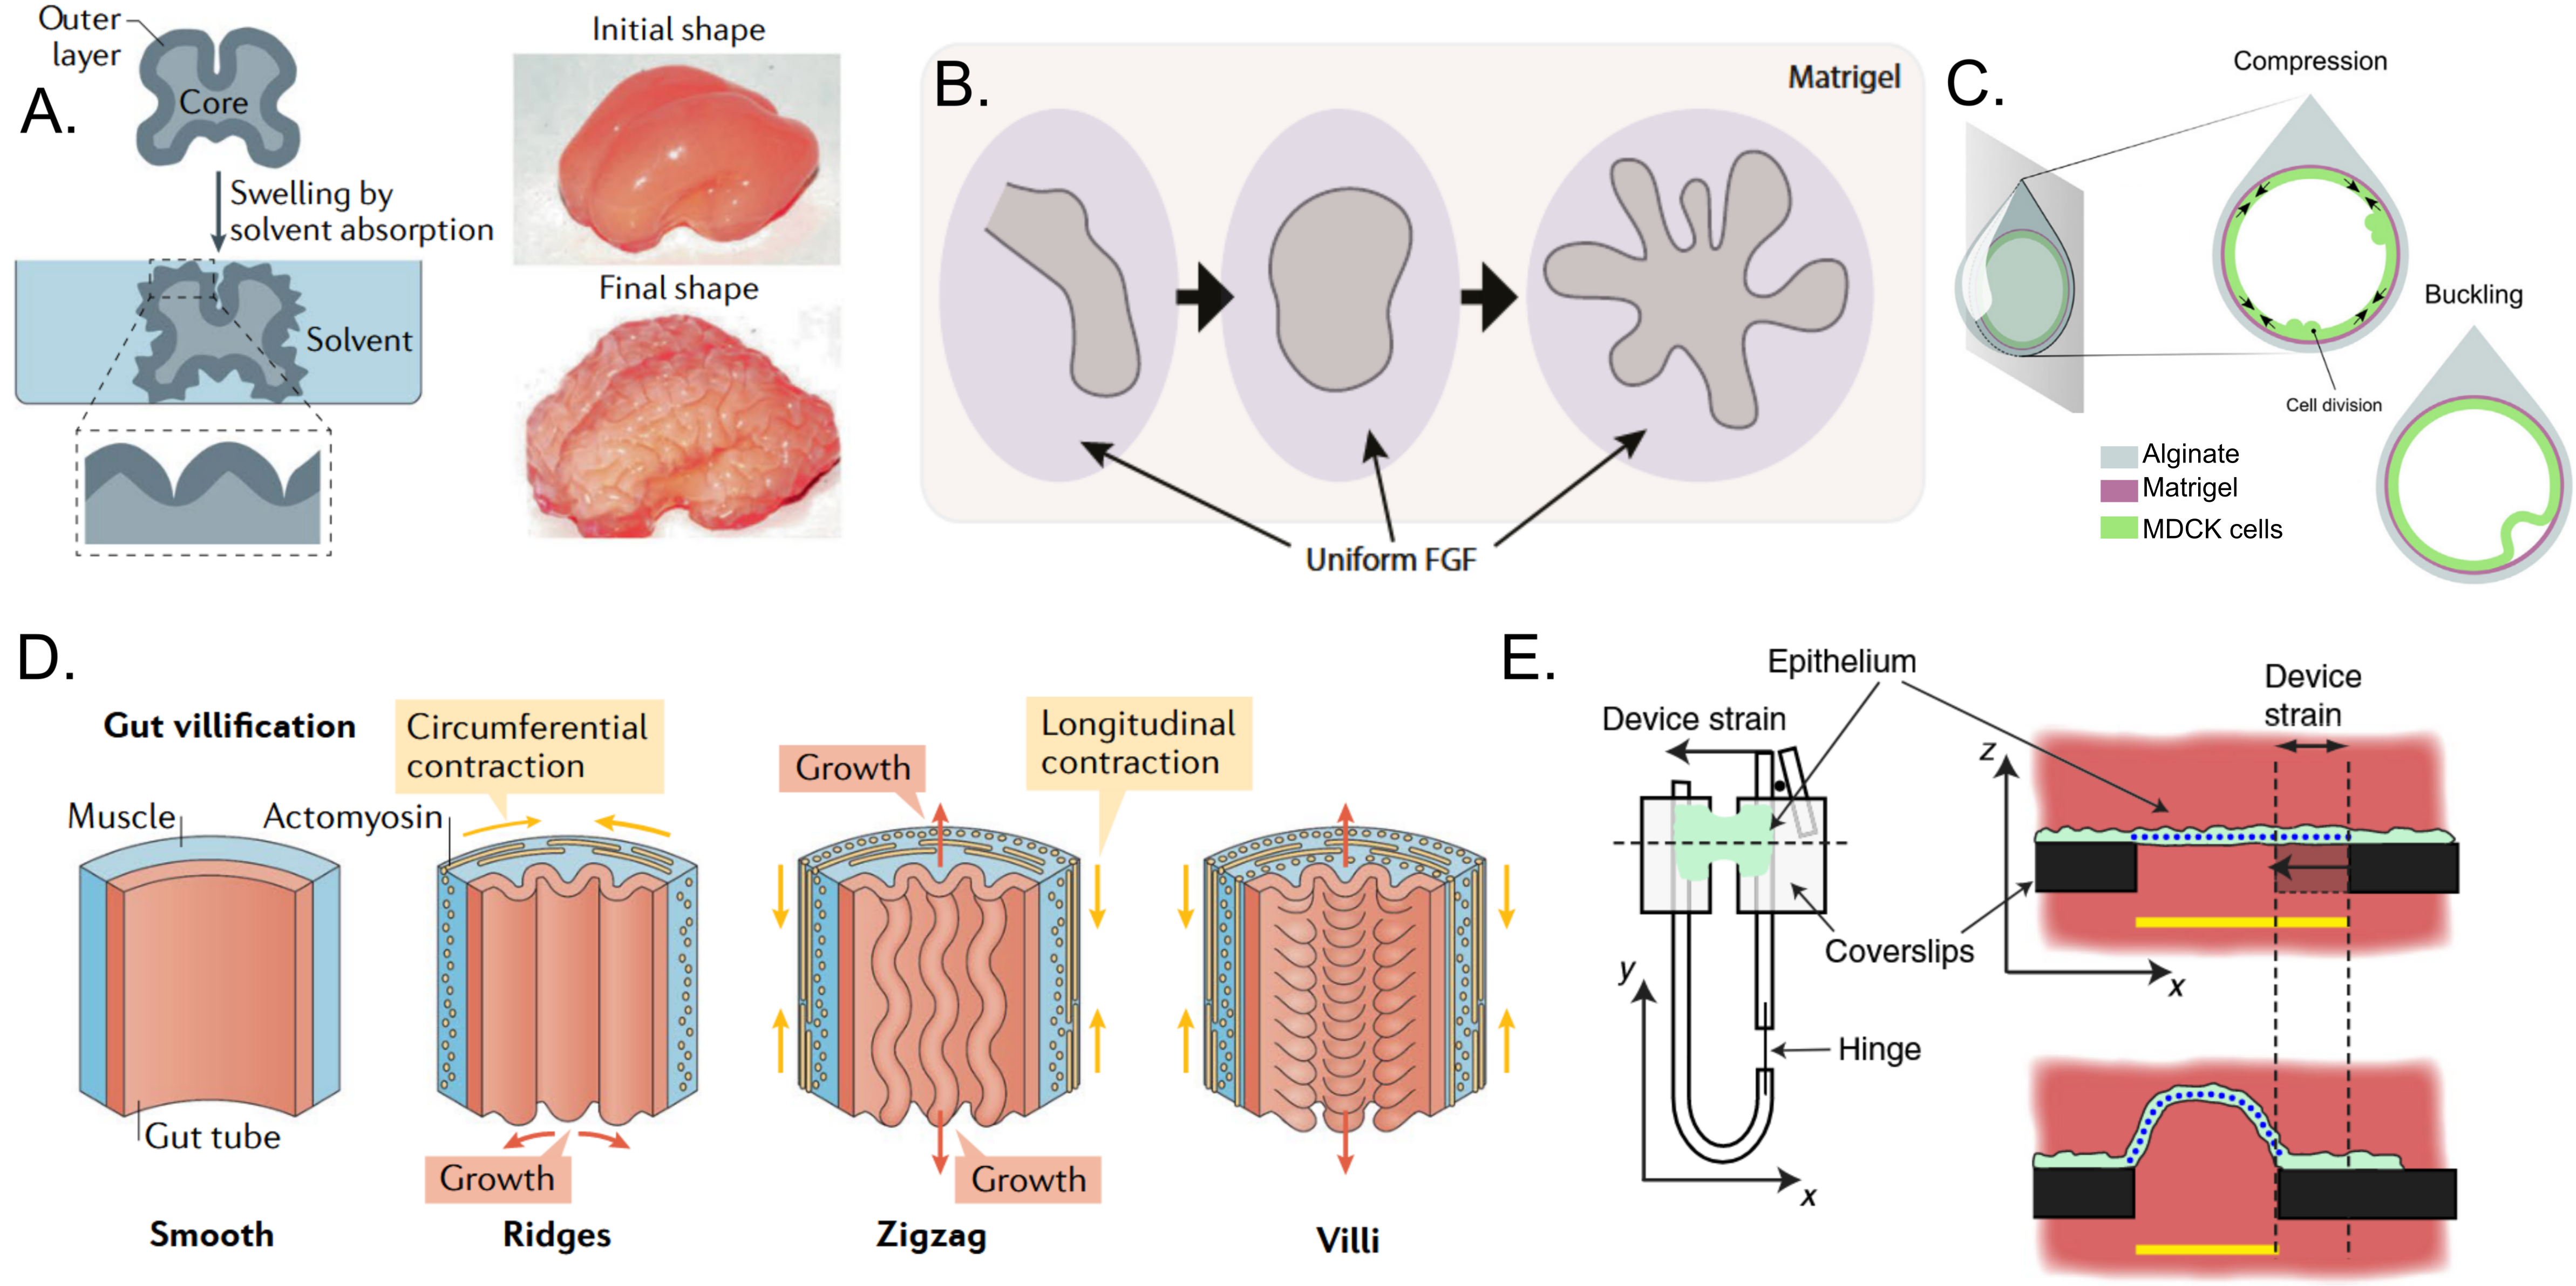
\includegraphics[width=\textwidth]{chap4buckling.png}
	\caption{\label{fig_4_6} \textbf{Examples of mechanical instabilities}: (A) Synthetic mini brains illustrate the wrinkling of the outer layer with swelling mimicking gyrification \cite{tallinen2016}. (B, D) Other way around where inner layer of lung or intestinal epithelia develops folds when embedded into a hydrogel or muscle shell \cite{varner2015, shyer2013}. (C) It is also shown that simple epithelial tissues embedded into a shell would also buckle \cite{trushko2020}. (D) \cite{wyatt2020} used matrix independent tissue with compression to illustrate that the epithelial tissue itself can undergo buckling. \textit{Panel A, D are adpated from \cite{collinet2021} and C from \cite{matejcic2020}}
	}
\end{figure}

The formation of the ventral furrow in the drosophila embryo can also be considered as a buckling event. Although there are multiple explanations for this phenomenon, recent studies have shown that the instability leading to the fold is caused by embryo-level forces \cite{guo2022, fierling2022}. Apart from instabilities, it is remarkable that the mechanical information can be encoded in the substrate. For instance, the tension produced by the cells in a pre-stretched membrane, on cutting would lead to curling \cite{tomba2022}, or through stretching a suspended epithelial layer would also do the same\cite{fouchard2020}.

It is noteworthy that there is currently only one established method for directly applying compressive stresses to suspended epithelial tissue. The Lab of Guillaume Charras has developed a technique using a cell-laden collagen gel sandwiched between two rods, where the gel is digested with collagenase to create a suspended monolayer (see fig \ref{fig_4_6} E). Through extensive experimentation, they have observed that the compression of more than 35\% strain produces transient buckling events \cite{wyatt2020}. Importantly, the actin cytoskeleton plays a crucial role in buffering deformations in this system.

\hypertarget{tissue-hydraulics}{%
	\section{Tissue hydraulics}\label{tissue-hydraulics}}

\hypertarget{hydraulic-control-of-morphogenesis}{%
	\subsection{Hydraulic control of morphogenesis}\label{hydraulic-control-of-morphogenesis}}


\begin{figure}
	\centering
	\includegraphics[width=\textwidth]{chap4hydraulics.png}
	\caption{\label{fig_4_7} \textbf{ Tissue hydraulics} plays an essential role in establishing (A) embryonic axis through lumen coarsening, and later the pressure regulates the size of the embryo. Laplace's law acts on the spherical cavities between cells to the whole blastocyst \cite{dumortier2019,chan2019, collinet2021}. (B) Interestingly, if the inflated structure is surrounded by a mesh you see a stressball effect, where material inflates through the mesh. Similar phenomena is visible in growth and inflation of the lizard lungs. The smooth muscle constrains the deformation leading to stressball morphogenesis \cite{palmer2021}. (C) In cnidarians, the different orientation of F-actin leads to different shapes of the organism \cite{stokkermans2022}.
	}
\end{figure}

In this thesis, we focus on the role of hydraulic pressure in morphogenesis. It has been well established in the field of developmental biology that fluid pressure plays a significant role in lumen expansion. For instance, in the mouse embryo, cell aggregates form small fluid cavities in intercellular junctions, which grow and coalesce into a large lumen, breaking the symmetry of the embryo, due to the presence of an osmotic pressure gradient (\cite{dumortier2019}; reviewed by \cite{torres-sanchez2021}, see fig \ref{fig_4_7} A). This process is powered by the pumping of ions and water by the cells, which generates pressure in the fluid-filled cavities, ultimately leading to the formation of spherical embryos. For any inflated spherical shell, the relationship between pressure ($\Delta P$), curvature ($R$), and surface tension ($\sigma$) can be described by Laplace's law. 
$$ \sigma = \frac{\Delta P R}{2}. $$ 
The shape that is created under pressure depends on the material properties of the tissue. For example, a homogeneous material would create a uniform curvature, such as a spherical shape, while an anisotropic tissue with oriented cells would result in various shapes, such as cylinders or ellipsoids \cite{stokkermans2021} (see fig\ref{fig_4_7} C). An interesting example of this phenomenon can be seen in the lobed epithelium of lizard lungs, which resembles the shape of a stress ball. Palmer et al. propose that the smooth muscle network functions as a mesh that constrains the epithelium, much like the outer layer of a stress ball \cite{palmer2021} (see fig\ref{fig_4_7} B). Upon the application of pressure, the epithelium inflates in the regions between the gaps in the muscles.

For embryos, an increase in pressure results in an increase in tension and stretching of the cells. Once a certain threshold is reached, the cell junctions may leak, causing a reduction in luminal pressure and shrinkage of the embryonic cavity. This system of pressure regulation through leakage acts as a mechanism for size regulation \cite{chan2019}. At the same time, it polarizes the embryo and promotes cell segregation and fate specification (see fig\ref{fig_4_7} A, reviewed by \cite{chan2020}).

Similar coalescence and lumen coarsening have been observed in other systems (reviewed in \cite{schliffka2019}). The pressure can also be generated through secretion of the matrix, as seen in the case of the drosophila hindgut with mucins \cite{syed2012}, or through the secretion of hyaluronic acid in the formation of ear canals in zebrafish otic vesicles \cite{munjal2021}. Despite numerous
\textit{in vivo} experiments, there are very few systems in which epithelial tissue can be subjected to controlled shape and size \textit{in vitro}.

\hypertarget{mechanics-of-domes}{%
	\subsection{Mechanics of domes}\label{mechanics-of-domes}}

\begin{figure}
	\centering
	\includegraphics[width=\textwidth]{chap4domes.png}
	\caption{\label{fig_4_8} \textbf{Historical development of epithelial domes}:(A) Distended epithelium was observed in explant cultures in 1930-50s. (B) With MDCK cell line, spontaneously forming domes/hemicysts were characterized \cite{leighton1969, valentich1979}. (C,D) In our lab, shape and size of the domes were controlled with micropatterning adhesion protein \cite{latorre2018}. The pressure and tension was measured with Laplace's law and traction force microscopy. (E-F) For non-spherical domes, curved monolayer stress microscopy technique was implemented by segmenting the dome shape \cite{marin-llaurado2022}.
	}
\end{figure}

Many of the morphogenetic events are called doming because the shape vaguely resemble a spherical cap. For instance, doming of the retina in the eye or zebrafish embryo, or doming during duct formation of mammary or salivary glands. There are typically two mechanisms for these: first, an accumulation of the cells or matrix to create curvature; and second, trans-epithelial transport causing hydraulic pressure-driven shape change. The second kind is remarkable as they mimic various lumenized epithelia \textit{in vivo}.

This is the most pertinent system to the thesis. I would briefly go into the historical developments in dome mechanics. 
	
Fluid-filled dome formation in epithelial tissue culture has been recorded since 1933 \cite{cameron1953} (see fig \ref{fig_4_8} A). After several decades alongside the development of cell culture techniques, microscopy, and MDCK cell line \footnote{It is very important to acknowledge the contribution of Madin-Darby canine kidney (MDCK) cells to the field of mechanobiology and enhancing our understanding of tissues \textit{in vitro}. Stewart H. Madin and Norman B. Darby, Jr. isolated female cocker spaniel dog’s kidney tubules cells in 1958. MDCK cells can self-organize in 2D and 3D; form monolayers and stratified layers; and undergo collective migrations. These cells are incredibly robust for experimentation.}, in 1968, Leighton and colleagues observed that the confluent MDCK cell monolayers formed hemispherical blisters (domes) \cite{leighton1969} (see fig \ref{fig_4_8} B). They observed that these are different from renal tubules because the apical surface, with microvilli, was facing outwards. They saw that these fluid-filled structures are dynamically changing size and curvature. They would burst to deflate and leak fluid out in the medium \cite{valentich1979}. After sometime, they could heal and form the dome again. Later, other cell lines derived from mammalian and amphibian kidneys were often observed to form domes too \cite{dulbecco1980, leighton1981, lever1979}
	
Now the mechanism is clear as the epithelial cells perform critical barrier function alongside controlling the transepithelial flow of ions and water. It was shown that hindering sodium-potassium ion pumping reduces the likelihood of domes \cite{leighton1969}. Thus, on forming a confluent monolayer these cells perform their function of pumping ions from apical to basal direction \cite{valentich1979}. If the substrate is solid and impermeable the tissue accumulates enough pressure to delaminate and form a spherical structure.

Most domes observed have been spherical and circular in footprint, indicating uniform tension across the dome. This can be explained by considering the dome as a thin shell under pressure, similar to a bubble, and following Laplace's law. Early studies attempted to infer tension through geometry and pressure measurement \cite{tanner1983}, finding that the pressure was of the same order as physiological vessels (see fig \ref{fig_4_9} A-B).

\begin{figure}
	\centering
	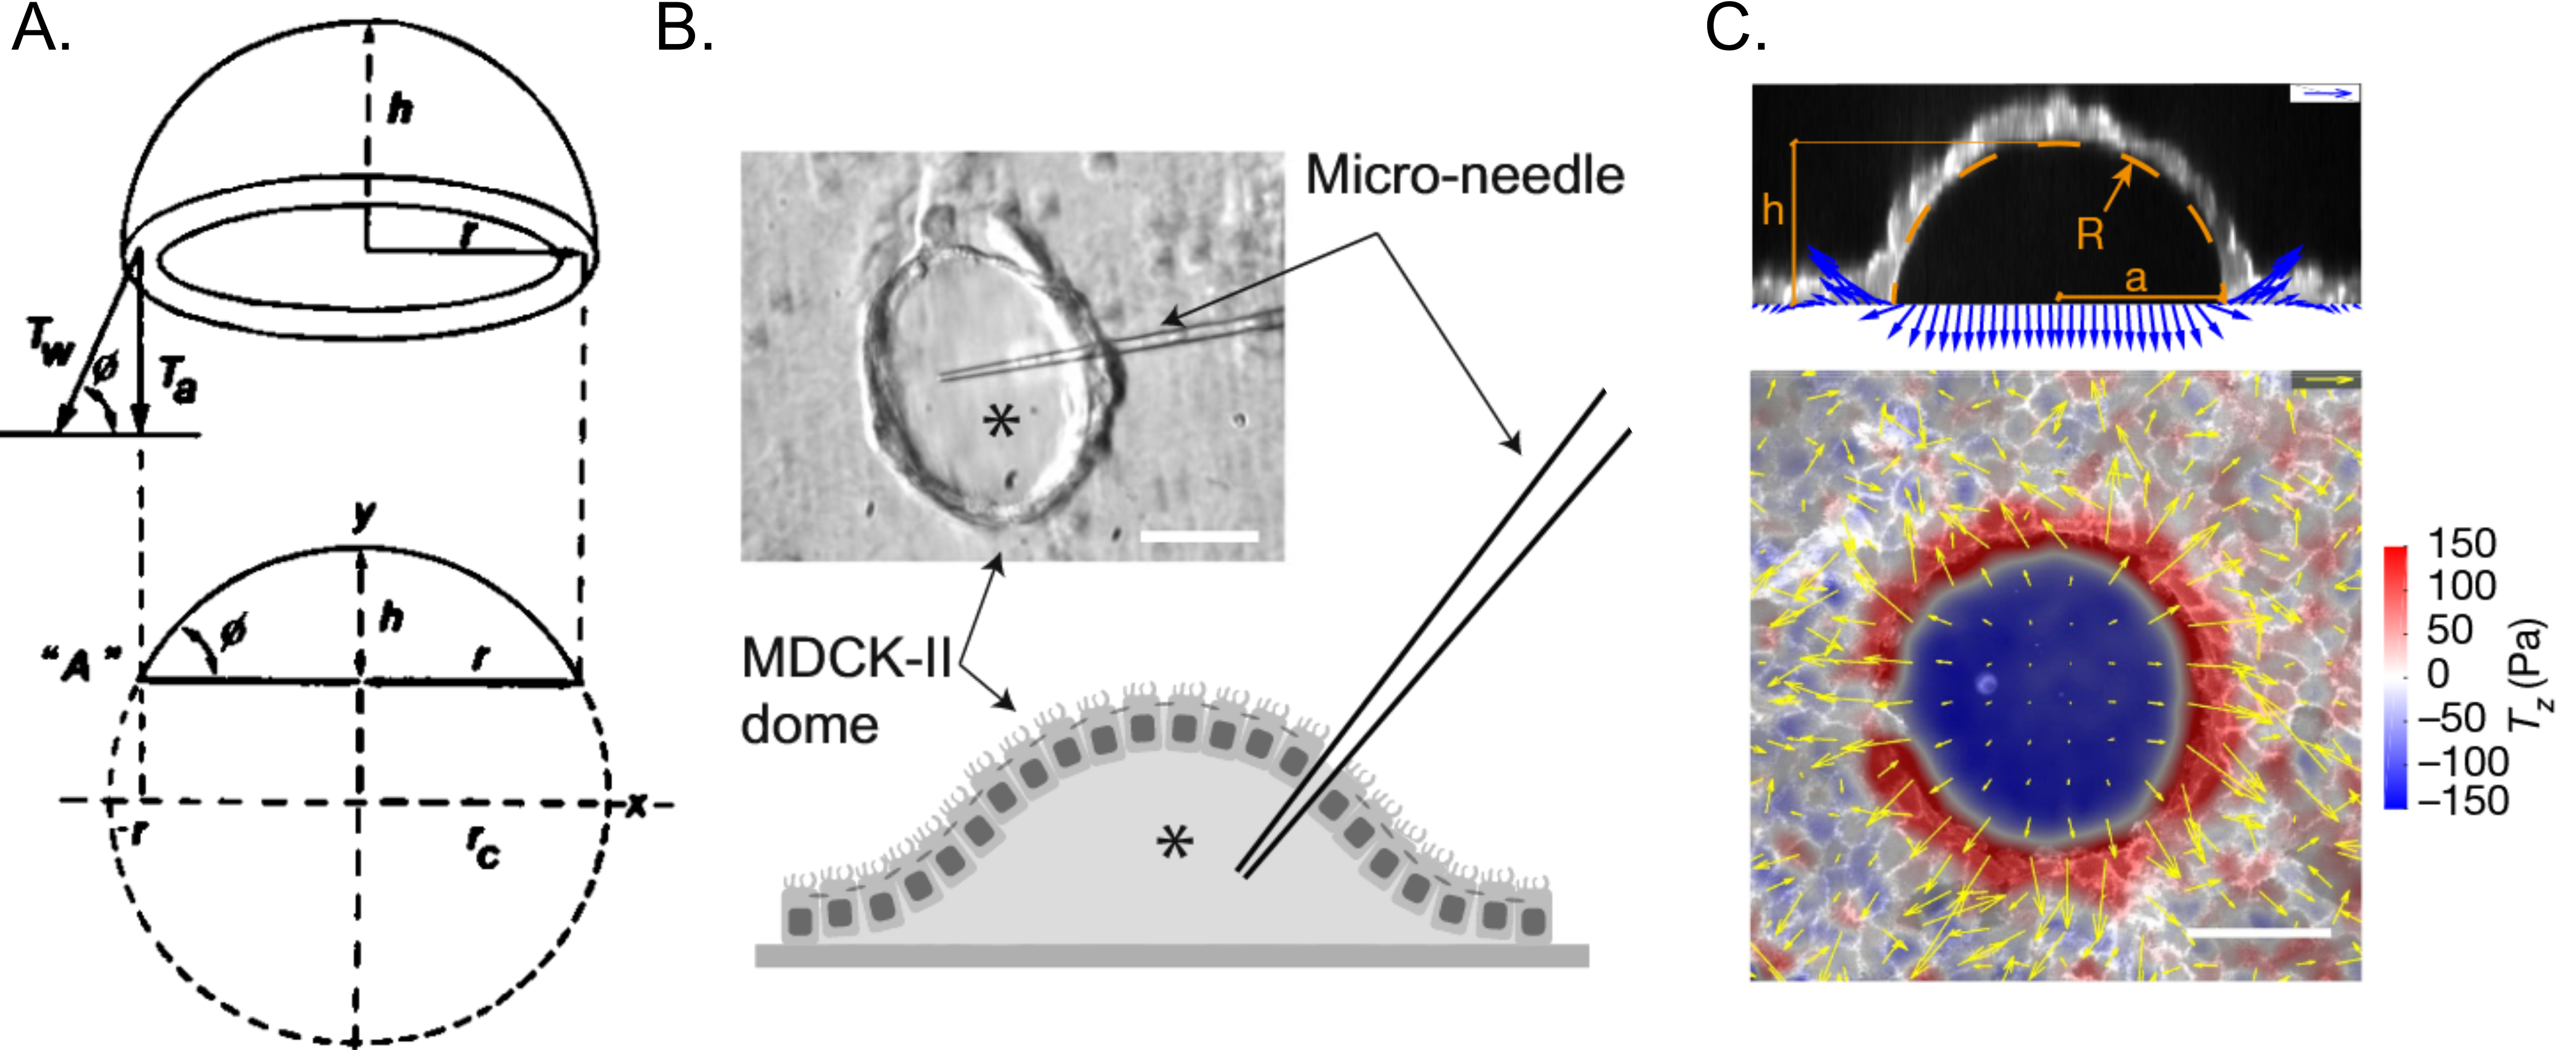
\includegraphics[width=\textwidth]{chap4pressure.png}
	\caption{\label{fig_4_9} \textbf{Methods for measuring pressure and tension}: (A) Earlier studies tried to estimate tension through geometry and thickness of the monolayer \cite{tanner1983}. (B) Later, pressure was measured by puncturing the dome with a micro-needle. However, the measurement of pressure is static, because the dome deflated after the puncturing \cite{choudhury2022}. (C) Traction force microscopy technique provides a viable non-invasive solution for measuring pressure under to domes \cite{latorre2018}.
	}
\end{figure}

One study \cite{popowicz1986} identified a ``dome curve'' when the frequency of domes was plotted against size, observing three classes of domes in terms of size. Smaller domes were observed to swell and increase in size. It was also suggested that there could be different subpopulations of MDCK cells. In the 1990s, many strains were characterized that formed different inflated structures, ranging from normal domes to tubules \cite{klebe1995}. One cell line, called super dome MDCK, formed larger domes.

Despite research into ion transport, hormone signaling, the role of tight junctions, and external shear stress, the understanding of the mechanics of domes and pressure has remained stagnant due to the lack of tools for measuring tension, pressure, and controlling the shape and size of these structures.

The work of Ernest Latorre in our laboratory has led to the development of a system for controlling the size of domes and studying the relationship between tension and pressure \cite{latorre2018} (see fig \ref{fig_4_8} C-D). By utilizing protein patterning techniques, Latorre was able to create non-adhesive circular regions on soft PDMS gel, which, when seeded with MDCK cells, led to the formation of domes. The gel was embedded with beads to allow for the calculation of traction forces and pressures exerted by the monolayer (see  fig \ref{fig_4_9} C). This system allowed for a deeper understanding of the rheology of tissue and the role of the cytoskeleton. He observed that stretching the actin cortex leads to dilution, and that tension reaches a stable value regardless of strain. He also observed the surprising phenomenon of superelasticity, where cells are heterogeneously stretched in the dome when tension is uniform. To further understand the role of actin and keratin bundles in providing superelasticity, Latorre et al. developed a vertex model through which they could understand the instability triggered by actin dilution, and rescued by intermediate filaments.

Ariadna Marin-Llaurado extended Latorre's work by examining domes of varying sizes and shapes (see fig \ref{fig_4_8} E). This study found that different-sized spherical domes have similar tensions, and that pressure is compensated according to curvature. Marin-Llaurado couldn't rely on a simple formula for tension calculation, because the tension in non-spherical domes is non-uniform \cite{marin-llaurado2022}. They used confocal microscopy to map dome curvature and calculated stresses computationally using a novel method called cMSM (curved Monolayer Stress Microscopy) (see fig \ref{fig_4_8} F). This method infers stresses just through geometry and pressure as in Young-Laplace relation. It does not need to make any assumptions related to material properties. The results showed that cells tended to align along the principal stress direction.

The mechanics of osmotic and hydraulic gradients are also crucial to understand. Chaudhary et al.~demonstrated that kidney cells act like a mechanobiological pump \cite{choudhury2022}. Using a two-layer microfluidic chip, the team was able to measure and apply pressure differences across an epithelial monolayer and observe that the tissue acted like a mechanical pump that stalls at high pressure. Remarkably, they discovered that diseased kidney cells pump in a different direction than healthy ones. They were able to control both osmotic and hydraulic pressure. Another study by Ishida-Ishihara et al.~investigated the connection between osmotic pressure and extracellular matrix swelling \cite{ishida-ishihara2020}. The researchers found that osmotic gradients trigger Aquaporin transport channels, leading to dome formation through Matrigel swelling. However, these domes are gel-filled structures that  differ from fluid-filled domes.

MDCK domes provide a model system for studying transport, cell fate, and tissue dynamics with a curvature. However, control over luminal pressure in these structures remains a challenge.

\hypertarget{what-is-to-be-done}{%
	\section{What is to be done?}\label{what-is-to-be-done}}

Morphogenesis refers to the process of tissue deformation or growth, which results from the combination of both endogenous and exogenous mechanical forces \cite{valet2022, collinet2021}. These forces may arise from the contractility of the epithelium and the surrounding matrix, as well as hydraulic pressure from the lumen \cite{torres-sanchez2021, chan2020}. The various stresses act on different components of the tissue, such as cells and the extracellular matrix, which exhibit unique viscoelastic properties and remodeling time scales \cite{cavanaugh2020, kelkar2020, ambrosi2019}. However, comprehending how these stresses interact with viscoelastic properties to bring about particular morphogenetic events in vivo presents significant technical and conceptual challenges. These obstacles include disentangling the roles played by distinct components in a system, a lack of tools for quantitative measurements of stresses and mechanical properties, and an inability to apply controlled stresses over a wide range of amplitudes and rates.

In response to these challenges, bottom-up approaches have emerged as a complementary strategy for understanding the morphogenetic potential of individual components and building complex, functional tissues \cite{trentesaux2023, ingber2018}. These approaches have been successful in engineering basic morphogenetic processes such as epithelial bending or buckling \cite{matejcic2022}. However, even though bottom-up approaches are proving to be successful, we still need tools that can measure and control the shape and stress of 3D epithelia simultaneously. Additionally, we lack computational models that integrate cellular and tissue shape with the subcellular determinants of epithelial mechanics, such as the contractility, turnover, and viscoelasticity of the actomyosin cortex.

This thesis seeks to address these gaps in knowledge by investigating the mechanics of epithelial tissues. A comprehensive understanding of the principles that govern tissue form and function is essential for both advancing our understanding of fundamental physical rules in biology and inspiring new engineering tools and design principles. To achieve this, we leverage cutting-edge technologies, such as 3D printing, microfluidics, and 3D cell cultures, to individually control morphogenetic driving factors. 

Our approach provides a material science perspective for probing the intricate mechanisms involved in the generation of forces and shape changes at the cellular and tissue levels, and holds promise for discovering emergent phenomena and enabling the building of novel tissue forms and assemblies.  

%	
%	\part{Results}
%	
	\part{Appendices}
	\begin{appendices}
		\renewcommand{\thesection}{A.\arabic{section}}
		\chapter{Methods and Materials}   \label{appendix_1}
		\section{Fabrication of microfluidic devices}
 
Polydimethylsiloxane (PDMS) gels (Sylgard PDMS kit, Dow Corning) were used to make the microfluidic devices. PDMS was synthesized by mixing the curing agent and elastomer in 1:9 weight ratio. This mixture was centrifuged for 2min at 900rpm to remove air bubbles. The unpolymerized PDMS was poured into a mold or spun to obtain the desired shape. 

There are four parts to the device (figgg). First is the top block, a thick PDMS block with four inlets and one channel for the application of hydraulic pressure. The second is a $200 \mu m$ thin PDMS layer with a $1.2mm$ diameter hole in the center with a $400nm$ porous membrane (Polycarbonate filtration membrane $0.4\mu m$, Whatman membranes) attached to it. The third is another $200 \mu m$ thin PDMS layer with a channel for seeding the cells. Lastly, all these PDMS parts are attached to, the fourth part, a glass-bottomed 35mm dish ($35mm, no. 1.5\#$ coverslip thickness, Cellvis). 

The top block was made using replica molding in a 3D printed mold. This mold was 3D printed with vat polymerization and a digital light processing 3D printer (Solus DLP 3D Printer with SolusProto resin). The mold’s surface was then silanized using Trichlorosilane (Trichloro(1H,1H,2H,2H-perfluorooctyl) silane, Merck) for preventing adhesion with unpolymerized PDMS. PDMS was poured into the mold and degassed for one hour. PDMS is cured with a hot plate at 100\textdegree{}C for $30min$. Once cured, PDMS is removed, cut into devices, and punched with $1.5mm$. $200\mu m$ thin PDMS layers were made by spin coating $4.5ml$ unpolymerized PDMS on a $15cm$ dish at $500rpm$ for $1min$. These dishes were incubated in an oven at 80\textdegree{}C to polymerize for 12hr. These thin sheets were cut into the parts of devices using a Silhouette cutting machine (Silhouette Cameo 4, Silhouette America). The sheets were attached to a Silhouette cutting mat and then Silhouette software was fed with the pattern of the device layers. A sharp cutting tool in the machine cut the PDMS along the pattern. These cut PDMS were peeled off with help of $70\%$ ethanol. 

These devices are assembled with the aid of ozone plasma cleaner (PCD-002-CE, Harrick Plasma). Glass bottomed dishes and thin PDMS layers with cell channels were treated for $1 min$ under plasma. Then bonded together by placing the layers in contact for $2 hr$ at 80\textdegree{}C. Similarly, the top block and thin membrane with porous membrane were also bonded. These layers were later bonded together again using plasma cleaner.

\section{Patterning protein on the device}
The devices were filled with $96\%$ ethanol for removing air bubbles. Then, devices are treated with $5\%$ v/v (3-aminopropyl) triethoxysilane (Merck) diluted in $96\%$ ethanol for $3min$ and rinse three times with $96\%$ ethanol. Later the devices were filled with MilliQ water to remove ethanol traces. PRIMO (Alveole Lab) was used to pattern adhesion-promoting protein. For this setup, devices were incubated with PLL (Poly-L-lysine solution, Merck) for $1hr$, subsequently with SVA PEG ($50mg/ml$ in $8.24pH$ HEPES) for $30min$, and rinsed with HEPES. Before using PRIMO, devices were filled with a photoinitiator. Desired protein pattern was loaded into the PRIMO software (Leonardo, Alveole Lab). 

PRIMO uses a microscope to shine the laser in the specific region according to the loaded pattern to cut PEG chains. After the PRIMO process, the samples were rinsed with phosphate-buffered saline (PBS, Merck). Then the samples were filled with fibronectin and fibrinogen ($100\mu g/ml$ Fibronectin in $2\%$ Far-red fibrinogen solution in 1X PBS) solution for $5 min$. Then samples were rinsed again with 1X PBS. Fibrinogen labels the fibronectin with Far-red signal to image the coated protein pattern and allows for tracking the position of the domes. The PRIMOed samples can be stored at 4\textdegree{}C for two to three days before seeding cells.

\section{Cell culture in the device}

To image cell shape and tissue structure Madin-Darby Canine Kidney (MDCK) cells expressing CIBN-GFP-CAAX were used for the experiments. CIBN-GFP-CAAX labels the plasma membrane. These cells were cultured in Dulbecco’s Modified Eagle Medium (DMEM, Gibco Thermofisher) with $10\%$ v/v fetal bovine serum (FBS, Gibco, Thermofisher), L-glutamine (Thermofisher), $100\mu g/ml$ streptomycin and penicillin. Cells were incubated at  37\textdegree{}C with a $5\%$ $CO_2$ condition. 

Before seeding cells in the device, it is filled with a cell culture medium. Cells are trypsinized and diluted at a concentration of $25-30\times10^6 cells/ml$. The cell channel of the device is filled with $30\mu l$ of cell solution and incubated for cell adhesion. After one hour of incubation, devices are rinsed with media to remove unattached cells. Devices were kept $24hr$ in the incubation for the growth of a monolayer before the experiment. It is important to note that the inverted epifluorescence microscope is need to see the cells. The bright-field microscope can not be used for visualizing cells because of the porous membrane.

\section{Staining actin with SPY-actin}

To observe the dynamics of the cortex, we used SPY555-actin (Spirochrome), a bright dye optimized for quick labeling of F-actin in live cells with low background. To prepare the 1000x solution, we added  $50\mu l$ of anhydrous DMSO to the stock SPY555-actin. We then added $1 \mu l$ of the 1000x solution to $999\mu l$ of cell culture medium. The resulting solution was introduced into the microfluidic chips and left in the incubator for 2 hours before imaging.

\section{Fabrication method for the Light-Sheet MOLI device }

The devices used with the light-sheet microscope consisted of a single PDMS block bonded to a glass microscope slide ($76 \times 26 mm$, RS Components BPB016). The blocks were made using a 3D printed mold (Ultimaker 3 with Ultimaker PLA Printer Filament 1616). PDMS was mixed, centrifuged, degassed, and cured as described above for the normal devices. Once cured, the PDMS was removed, cut into individual devices and punched with a 1.5mm biopsy punch. The PDMS blocks were then attached glass slides using a thin layer of unpolymerized PDMS, that was coated onto the glass slides using a spatula. The devices were then kept on a hotplate at 100\textdegree{}C for $30min$ to allow the PDMS bonding to fully cure. The $400nm$ porous membranes were then attached to the devices. The edges of the membrane were carefully dipped into unpolymerized PDMS, before being placed flat on the top of the device. Particular care was taken to ensure the center of the membrane over the punched pressure-application hole remained free of PDMS. The devices were then kept at  65\textdegree{}C for an hour to allow the PDMS bonding to fully cure.

\section{Device protein patterning and cell culture in Light-Sheet device}

The light-sheet devices were protein patterned and cell cultured using the same methods and steps as outlined above for the normal devices, with the one minor addition of the use of a simple PDMS and glass cap for a few critical steps. The porous membrane for pressure application, and thus the site of protein patterning and cell seeding, for the light-sheet devices is exposed and on the top side of the devices. This mostly allowed for easy application of reagents as a droplet could be applied and aspirated directly. 

However for the more sensitive steps in the procedure, a simple PDMS and glass device was used to create a temporary covered channel over the porous membrane to regulate the procedure and ensure the treatment of the devices was highly standardized. Specifically, the cap was used for the application of photoinitiator during PRIMO, and for the application of cell solution during cell attachment. The caps were fabricated using $2cm\times2cm$ squares of a $400\mu m$ thick PDMS layer, with a keyhole shape cut in from the side. Each PDMS piece was then stuck to a $18mm$ diameter coverslip ($18mm$, $1\#$ Cover glasses circular, Marienfeld 0111580) using the surface tension of the liquid. The experimental apparatus and measurements for the light-sheet devices were the same as the normal devices as outlined above.

\section{Application and measurement of the pressure}

The pressure is applied via hydrostatic forces similar to the previous studies \cite{choudhury2022, palmer2021}. The two channels in the chip were separated by the porous membrane. Cells are on the bottom side of the membrane. The pressure in the channel (top side of the membrane) is used to inflate the structures on the top. This channel has one inlet and one outlet for removing bubbles. The inlet is connected to a $35 ml$ reservoir of cell culture medium (in a $50 ml$ falcon tube) by tubing (PTFE Tubing $1/16  inch$ OD for Microfluidics, Darwin microfluidics) and the outlet is connected to a shutoff valve (Microfluidic Sample Injection / Shut-off Valve, Darwin microfluidics). Once bubbles are removed, closing the valve would apply the pressure on the basal side of the cells according to the difference between the height of the fluid level. All tubings are connected to the chip with a steel insert (Stainless steel 90deg Bent PDMS Couplers, Darwin microfluidics). We are able to find zero by matching the height of the device to the liquid and air interface in the reservoir. This is confirmed with the experiments, where on applying pressure domes form but on slow reduction in pressure to zero causes domes to deflate.

\section{Confocal Microscopy}

For timelapse imaging of domes at a larger time interval (> 1 min), an inverted Nikon microscope with a spinning disk confocal unit (CSU-W1, Yokogawa) was used with Nikon 40x, 20x, and 10x air lenses. For shorter time intervals (< 10 s), a Zeiss LSM880 inverted confocal microscope was used with laser scanning mode. Fast imaging was enabled by imaging a single line in the middle of the dome. 

\section{Light-sheet microscopy}

The imaging of the light-sheet devices was done with a dual-illumination inverted Selective Plane Illumination Microscope (diSPIM) (QuVi SPIM, Luxendo, Brucker) with Nikon 40x immersion lenses (Nikon CFI Apo 40x W 0.8 NA NIR water immersion objective). For the buckling experiments, only single objective illumination and detection was used for the fast imaging of $2 s/frame$. 

\section{Quantification of the dome areal strain and tension}

As mentioned earlier, the domes were imaged in 3D with confocal microscopy. We used ImageJ to manually section the dome in the middle in the YZ plane, XZ plane is a plane parallel to the monolayer, with Reslice function along the Z axis. This section was used to calculate the height (h), radius of curvature (R), and base radius (a). Strain ($\epsilon$) and tension ($\sigma$) were calculated as,
$$\epsilon = \frac{h^2}{a^2}, \ \ \ \ and \ \ \ \ \sigma = \frac{\Delta P R}{2}.$$
The raw data was extracted in ImageJ and then MATLAB was used to compute and plot the strain and tension.

\section{Analysis of the kymographs}

For cyclic pressure or buckling experiments, the domes were imaged at low resolution and high noise levels to capture fast dynamics. The previous method of manually quantifying each time point is not feasible. Thus, we used the ImageJ function of the Reslice function along the time axis. We resliced it along the Y-time axis in the middle of the dome, such that we get a kymograph of height as a function of time. Also, we performed the reslicing along the XT axis at the plane of the monolayer, such that we get the kymograph of the base radius with respect to time. These kymographs were in form of images save manually with ImageJ. 

A custom-built MATLAB code was used to digitize the kymographs, where maximum intensity along each time was considered as the current dome height position. The first $30 s$ of the experiment pressure is zero, so the unstretched monolayer position is determined from those time points. Dome height is calculated with the difference between the current position and the initial position. Base radius is calculated similarly by subtracting two sides. The radius of curvature is calculated using the relation between the base and height of the dome as
$$R=(h^2+a^2)/2h.$$


\section{Qualitative analysis of the buckling event}

Whether domes are buckling or not was determined manually checking every frame during the deflation. If dome maintains the smooth circular geometry in XZ plane during the deflation, we mark the dome as “not buckling”. However, if the dome has a visual discontinuity in the curvature or a kink it is then considered to be “buckling”.

Imaging the fast events in XY plane was done in an ad hoc manner. To capture the folds, the dome as imaged closer to the apical surface of the monolayer. The type of fold was determined by carefully observing the way which monolayer makes contact with the imaging plane. If there is one point of contact in the center and spreads outwards, it is considered as accumulation along the periphery. In case where there are multiple points of contact and they all join in the middle, it is considered as a network of folds.
	\end{appendices}
	
	%%% Backmatter %%%
	\backmatter
	\bibliography{LaCaN/9800-Bibliography/9800-Bibliography}
	
\end{document}



